%!TEX root = ../thesis.tex

\graphicspath{{assets/chapter_3/}}

\chapter{\glsfmtshort{ris}-Aided \glsfmtshort{swipt}: Joint Waveform and Beamforming Design}\label{ch:ris_aided_swipt}

\begin{section}{Introduction}
	\begin{subsection}{\glsfmtlong{swipt}}
		With the great advance in communication performance, a bottleneck of wireless networks has come to energy supply. \gls{swipt} is a promising solution to connect and power mobile devices via \gls{rf} waves. It provides low power at \si{\uW} level but broad coverage up to hundreds of meters in a sustainable and controllable manner, bringing more opportunities to the \gls{iot} and \gls{m2m} networks. The upsurge in wireless devices, together with the decrease of electronics power consumption, calls for a re-thinking of future wireless networks based on \gls{wpt} and \gls{swipt} \cite{Clerckx2019}.

		The concept of \gls{swipt} was first cast in \cite{Varshney2008}, where the authors investigated the \gls{r-e} tradeoff for a flat Gaussian channel and typical discrete channels. \cite{Zhou2013} proposed two practical co-located information and power receivers, i.e., \gls{ts} and \gls{ps}. Dedicated information and energy beamforming were then investigated in \cite{Zhang2013,Park2014} to characterize the \gls{r-e} region for multi-antenna broadcast and interference channels. On the other hand, \cite{Trotter2009} pointed out that the \gls{rf}-to-\gls{dc} conversion efficiency of rectifiers depends on the input power and waveform shape. It implies that the modeling of the energy harvester, particularly its nonlinearity, has a crucial impact on the waveform preference, resource allocation, and system design of any wireless-powered systems \cite{Trotter2009,Clerckx2018,Clerckx2019}. Motivated by this, \cite{Clerckx2016a} derived a tractable nonlinear harvester model based on the Taylor expansion of diode I-V characteristics, and performed joint waveform and beamforming design for \gls{wpt}. Simulation and experiments showed the benefit of modeling energy harvester nonlinearity in real system design \cite{Kim2019,Kim2020a} and demonstrated the joint waveform and beamforming strategy as a key technique to expand the operation range \cite{Kim2021}. A low-complexity adaptive waveform design by \gls{smf} was proposed in \cite{Clerckx2017} to exploit the rectifier nonlinearity, whose advantage was then demonstrated in a prototype with channel acquisition \cite{Kim2017}. Beyond \gls{wpt}, \cite{Clerckx2018b} uniquely showed that the rectifier nonlinearity brings radical changes to \gls{swipt} design, namely (i) modulated and unmodulated waveforms are not equally suitable for wireless power delivery; (ii) a multi-carrier unmodulated waveform superposed to a multi-carrier modulated waveform can enlarge the \gls{r-e} region; (iii) a combination of \gls{ps} and \gls{ts} is generally the best strategy; (iv) the optimal input distribution is not the conventional \gls{cscg}; (v) modeling rectifier nonlinearity is beneficial to system performance and essential to efficient \gls{swipt} design. Those observations, validated experimentally in \cite{Kim2019}, led to the question: \emph{What is the optimal input distribution for \gls{swipt} under nonlinearity?} This question was answered in \cite{Varasteh2020} for single-carrier \gls{swipt}, and some attempts were further made in \cite{Varasteh2019d} for multi-carrier \gls{swipt}. The answers shed new light to the fundamental limits of \gls{swipt} and practical signaling (e.g., modulation and waveform) strategies. It is now well understood from \cite{Clerckx2018b,Varasteh2020,Varasteh2019d} that, due to harvester nonlinearity, a combination of \gls{cscg} and on-off keying in single-carrier setting and non-zero mean asymmetric inputs in multi-carrier setting lead to significantly larger \gls{r-e} region compared to conventional \gls{cscg}. Recently, \cite{Varasteh2020a} used machine learning techniques to design \gls{swipt} signaling under nonlinearity to complement the information-theoretic results of \cite{Varasteh2020}, and new modulation schemes were subsequently invented.
	\end{subsection}





	\begin{subsection}{\glsfmtlong{ris}}
		\gls{ris} has recently emerged as a promising technique that adapts the propagation environment to enhance the spectrum and energy efficiency. In practice, a \gls{ris} consists of multiple individual sub-wavelength reflecting elements to adjust the amplitude and phase of the incoming signal (i.e., passive beamforming). Different from the relay, backscatter and frequency-selective surface \cite{Anwar2018}, the \gls{ris} assists the primary transmission using passive components with negligible thermal noise but is limited to frequency-dependent reflection.

		Inspired by the development of real-time reconfigurable metamaterials \cite{Cui2014}, the authors of \cite{Liaskos2018} introduced a programmable metasurface that steers or polarizes the electromagnetic wave at a specific frequency to mitigate signal attenuation. \cite{Wu2018} proposed a \gls{ris}-assisted \gls{miso} system and jointly optimized the precoder at the \gls{ap} and the phase shifts at the \gls{ris} to minimize the transmit power. The active and passive beamforming problem was then extended to the discrete phase shift case \cite{Wu2019a} and the multi-user case \cite{Wu2019}. In \cite{Abeywickrama2020}, the authors investigated the impact of non-zero resistance on the reflection pattern and emphasized the coupling between reflection amplitude and phase shift in practice. To estimate the cascaded \gls{ap}-\gls{ris}-\gls{ue} link without \gls{rf}-chains at the \gls{ris}, practical protocols were developed based on element-wise on/off switching \cite{Nadeem2019}, training sequence and reflection pattern design \cite{You2019,Kang2020}, and compressed sensing \cite{Wang2020}. The hardware architecture, design challenges, and application opportunities of practical \gls{ris} were covered in \cite{Wu2020}. In \cite{Dai2020}, a prototype \gls{ris} with \num{256} \num{2}-bit elements based on \gls{pin} diodes was developed to support real-time video transmission at \si{GHz} and mmWave frequency.
	\end{subsection}


	\begin{subsection}{\glsfmtshort{ris}-Aided \glsfmtshort{swipt}}
		By integrating \gls{ris} with \gls{swipt}, the constructive reflection can boost the end-to-end power efficiency and improve the \gls{r-e} tradeoff. In multi-user cases, dedicated energy beams were proved unnecessary for the weighted sum-power maximization \cite{Wu2020b} but essential when fairness issue is considered \cite{Tang2019}. It was also claimed that \gls{los} links could boost the power efficiency since rank-deficient channels require fewer energy beams \cite{Wu2020a}. However, \cite{Wu2020b,Tang2019,Wu2020a} were based on a linear energy harvester model that is known in both the \gls{rf} and the communication literature to be inefficient and inaccurate \cite{Clerckx2019,Trotter2009,Clerckx2018,Clerckx2016a,Kim2019,Kim2020a,Kim2021,Clerckx2017,Kim2017,Clerckx2018b,Varasteh2020,Varasteh2019d,Varasteh2020a}. Based on practical \gls{ris} and harvester models, \cite{Xu2021c} introduced a scalable resource allocation framework for a large-scale tile-based \gls{ris}-assisted \gls{swipt} system, where the optimization consists of a reflection design stage and a joint reflection selection and precoder design stage. The proposed framework provides a flexible tradeoff between performance and complexity. To the best of our knowledge, all existing papers considered resource allocation and beamforming design for dedicated information and energy users in a single-carrier network. In this paper, we instead build our design based on a proper nonlinear harvester model that captures the dependency of the output \gls{dc} power on both the power and shape of the input waveform, and marry the benefits of joint multi-carrier waveform and active beamforming optimization for \gls{swipt} with the passive beamforming capability of \gls{ris}, to investigate the \gls{r-e} tradeoff for one \gls{swipt} user with co-located information decoder and energy harvester. We ask ourselves the important question: \emph{How to jointly exploit the spatial domain and the frequency domain efficiently through joint waveform and beamforming design to enlarge the \gls{r-e} region of \gls{ris}-aided \gls{swipt}?} The contributions of this paper are summarized as follows.

		\emph{First,} we propose a novel \gls{ris}-aided \gls{swipt} architecture based on joint waveform, active and passive beamforming design under the diode nonlinear model \cite{Clerckx2016a}. Although this tractable harvester model accurately reveals how the input power level and waveform shape influence the output \gls{dc} power, it also introduces design challenges such as frequency coupling (i.e., components of different frequencies compensate and produce \gls{dc}), waveform coupling (i.e., different waveforms jointly contribute to \gls{dc}), and high-order objective function. To make an efficient use of the rectifier nonlinearity, we superpose a multi-carrier unmodulated power waveform (deterministic multisine) to a multi-carrier modulated information waveform and evaluate the performance under the \gls{ts} and \gls{ps} receiving modes. The proposed joint waveform, active and passive beamforming architecture exploits the rectifier nonlinearity, the channel selectivity, and a beamforming gain across frequency and spatial domains to enlarge the achievable \gls{r-e} region. This is the first paper to propose a joint waveform, active and passive beamforming architecture for \gls{ris}-aided \gls{swipt}.

		\emph{Second,} we characterize each \gls{r-e} boundary point by energy maximization under a rate constraint. The problem is solved by a \gls{bcd} algorithm based on the \gls{csit}. For active beamforming, we prove that the global optimal active information and power precoders coincide at \gls{mrt} even with rectifier nonlinearity. For passive beamforming, we propose a \gls{sca} algorithm and retrieve the \gls{ris} phase shift by eigen decomposition with optimality proof. Finally, the superposed waveform and the splitting ratio are optimized by the \gls{gp} technique. The \gls{ris} phase shift, active precoder, and waveform amplitude are updated iteratively until convergence. This is the first paper to jointly optimize waveform and active/passive beamforming in \gls{ris}-aided \gls{swipt}.

		\emph{Third,} we introduce two closed-form adaptive waveform schemes to avoid the exponential complexity of the \gls{gp} algorithm. To facilitate practical \gls{swipt} implementation, the \gls{wf} strategy for modulated waveform and the \gls{smf} strategy for multisine waveform are combined in time and power domains, respectively. The passive beamforming design is also adapted to accommodate the low-complexity waveform schemes. The proposed low-complexity \gls{bcd} algorithm achieves a good balance between performance and complexity.

		\emph{Fourth,} we provide numerical results to evaluate the proposed algorithms. It is concluded that (i) \gls{ris} enables constructive reflection and flexible subchannel design in the frequency domain that is essential for \gls{swipt} systems; (ii) \gls{ris} mainly affects the effective channel instead of the waveform design; (iii) multisine waveform is beneficial to energy transfer especially when the number of subbands is large; (iv) \gls{ts} is preferred at low \gls{snr} while \gls{ps} is preferred at high \gls{snr}; (v) there exist two optimal \gls{ris} development locations, one close to the \gls{ap} and one close to the \gls{ue}; (vi) the output \gls{snr} scales linearly with the number of transmit antennas and quadratically with the number of \gls{ris} elements; (vii) due to the rectifier nonlinearity, the output \gls{dc} scales quadratically with the number of transmit antennas and quartically with the number of \gls{ris} elements; (viii) for narrowband \gls{swipt}, the optimal active and passive beamforming for any \gls{r-e} point are also optimal for the whole \gls{r-e} region; (ix) for broadband \gls{swipt}, the optimal active and passive beamforming depend on specific \gls{r-e} point and require adaptive designs; (x) the proposed algorithms are robust to practical impairments such as inaccurate cascaded \gls{csit} and finite \gls{ris} reflection states.
	\end{subsection}
\end{section}

\begin{section}{System Model}\label{se:system_model}
	\begin{figure}[!t]
		\centering
		\def\svgwidth{0.9\columnwidth}
		\input{assets/chapter_3/system.eps_tex}
		\caption{An \gls{ris}-aided multi-carrier \gls{miso} \gls{swipt} system.}
		\label{fi:system}
	\end{figure}

	As shown in Fig.~\ref{fi:system}, we propose a \gls{ris}-aided \gls{swipt} system where an $M$-antenna \gls{ap} delivers information and power simultaneously, through an $L$-element \gls{ris}, to a single-antenna \gls{ue} over $N$ orthogonal evenly-spaced subbands. We consider a quasi-static block fading model and assume the \gls{csit} of direct and cascaded channels is known. The signals reflected by two or more times are omitted, and the noise power is assumed too small to be harvested.


	\begin{subsection}{Transmitted Signal}
		Following \cite{Clerckx2018b}, we superpose a multi-carrier modulated information-bearing waveform to a multi-carrier unmodulated power-dedicated deterministic multisine to boost the spectrum and energy efficiency. The information signal transmitted over subband $n \in \{1, \dots, N\}$ at time $t$ is
		\begin{equation}
			\boldsymbol{x}_{\mathrm{I},n}(t) = \Re\left\{\boldsymbol{w}_{\mathrm{I},n} \tilde{x}_{\mathrm{I},n}(t) e^{j2{\pi}{f_n}{t}}\right\},
		\end{equation}
		where $\boldsymbol{w}_{\mathrm{I},n} \in \mathbb{C}^{M \times 1}$ is the information precoder at subband $n$, $\tilde{x}_{\mathrm{I},n}\sim\mathcal{CN}(0,1)$ is the information symbol at subband $n$, and $f_n$ is the frequency of subband $n$. On the other hand, the power signal transmitted over subband $n$ at time $t$ is
		\begin{equation}
			\boldsymbol{x}_{\mathrm{P},n}(t) = \Re\left\{\boldsymbol{w}_{\mathrm{P},n} e^{j2{\pi}{f_n}{t}}\right\},
		\end{equation}
		where $\boldsymbol{w}_{\mathrm{P},n} \in \mathbb{C}^{M \times 1}$ is the power precoder at subband $n$. Therefore, the superposed signal transmitted over all subbands at time $t$ is
		\begin{equation}
			\boldsymbol{x}(t) = \Re{\left\{\sum_{n=1}^N(\boldsymbol{w}_{\mathrm{I},n}\tilde{x}_{\mathrm{I},n}(t)+\boldsymbol{w}_{\mathrm{P},n}){e^{j2{\pi}{f_n}{t}}}\right\}}.
		\end{equation}
		We also define $\boldsymbol{w}_{\mathrm{I/P}} \triangleq [\boldsymbol{w}_{\mathrm{I/P},1}^T,\dots,\boldsymbol{w}_{\mathrm{I/P},N}^T]^T \in \mathbb{C}^{MN \times 1}$.
	\end{subsection}


	\begin{subsection}{Reflection Pattern and Composite Channel}
		According to Green's decomposition \cite{Hansen1989}, the backscattered signal of an antenna can be decomposed into the \emph{structural mode} component and the \emph{antenna mode} component. The former is fixed and can be regarded as part of the environment multipath, while the latter is adjustable and depends on the mismatch of the antenna and load impedance. \gls{ris} element $l \in \{1, \dots, L\}$ varies its impedance $Z_l = R_l + j X_l$ to reflect the incoming signal, and the reflection coefficient is defined as
		\begin{equation}
			\phi_l = \frac{Z_l - Z_0}{Z_l + Z_0} \triangleq \eta_l e^{j\theta_l},
		\end{equation}
		where $Z_0$ is the real-valued characteristic impedance, $\eta_l \in [0, 1]$ is the reflection amplitude,\footnote{Due to the non-zero power consumption at the \gls{ris}, $R_l > 0$ in practice such that $\eta_l < 1$ and is a function of $\theta_l$. This paper sticks to the most common \gls{ris} model where the reflection amplitude equals \num{1} so as to reduce the design complexity and provide a primary benchmark for practical \gls{ris}-aided \gls{swipt}.} and $\theta_l \in [0,2\pi)$ is the phase shift. We also define $\boldsymbol{\phi} \triangleq [\phi_1, \dots, \phi_L]^H \in \mathbb{C}^{L \times 1}$ and $\boldsymbol{\Theta} \triangleq \mathrm{diag}(\phi_1, \dots, \phi_L)=\mathrm{diag}(\boldsymbol{\Phi}^*) \in \mathbb{C}^{L \times L}$ as the \gls{ris} vector and matrix, respectively.

		\begin{remark}\label{re:reflection_coefficient}
			The element impedance $Z_l$ maps to the reflection coefficient $\phi_l$ uniquely. Since the reactance $X_l$ depends on the frequency, the reflection coefficient $\phi_l$ is also a function of frequency and cannot be designed independently at different subbands. In this paper, we assume the bandwidth is small compared to the operating frequency such that the reflection coefficient of each \gls{ris} element is the same at all subbands.
		\end{remark}

		At subband $n$, we denote the \gls{ap}-\gls{ue} direct channel as $\boldsymbol{h}_{\mathrm{D},n}^H \in \mathbb{C}^{1 \times M}$, the \gls{ap}-\gls{ris} incident channel as $\boldsymbol{H}_{\mathrm{I},n} \in \mathbb{C}^{L \times M}$, and the \gls{ris}-\gls{ue} reflected channel as $\boldsymbol{h}_{\mathrm{R},n}^H \in \mathbb{C}^{1 \times L}$. The auxiliary \gls{ap}-\gls{ris}-\gls{ue} link can be modeled as a concatenation of the incident channel, the \gls{ris} reflection, and the reflected channel. Hence, the composite equivalent channel reduces to
		\begin{equation}\label{eq:h_n}
			\boldsymbol{h}_{n}^H = \boldsymbol{h}_{\mathrm{D},n}^H + \boldsymbol{h}_{\mathrm{R},n}^H \boldsymbol{\Theta} \boldsymbol{H}_{\mathrm{I},n} = \boldsymbol{h}_{\mathrm{D},n}^H + \boldsymbol{\phi}^H \boldsymbol{V}_{n},
		\end{equation}
		where we define the cascaded incident-reflected channel at subband $n$ as $\boldsymbol{V}_{n} \triangleq \mathrm{diag}(\boldsymbol{h}_{\mathrm{R},n}^H)\boldsymbol{H}_{\mathrm{I},n} \in \mathbb{C}^{L \times M}$. We also define $\boldsymbol{h} \triangleq [\boldsymbol{h}_1^T,\dots,\boldsymbol{h}_N^T]^T \in \mathbb{C}^{MN \times 1}$.

		\begin{remark}\label{re:subband_tradeoff}
			The cascaded channel varies at different subbands, but the reflection cannot be designed independently at different frequencies. Therefore, there exists a tradeoff for the passive beamforming design in the frequency domain, and the composite subchannels should be tuned adaptively to meet the specific requirement of multi-carrier \gls{swipt}. For example, one can design the reflection pattern to either enhance the strongest subband (e.g., $\max_{\boldsymbol{\phi},n} \lVert \boldsymbol{h}_n \rVert$), or improve the fairness among subbands (e.g., $\max_{\boldsymbol{\phi}} \min_n \lVert \boldsymbol{h}_n \rVert$). That is to say, \gls{ris} essentially enables a flexible subchannel design. In the \gls{miso} case, a similar effect also exists in the spatial domain. Therefore, each reflection coefficient is indeed shared by $M$ antennas over $N$ subbands.
		\end{remark}
	\end{subsection}


	\begin{subsection}{Received Signal}
		The received superposed signal at the single-antenna \gls{ue} is\footnote{We assume that the time difference of signal arrival via direct and auxiliary link is negligible compared to the symbol period.}
		\begin{equation}
			y(t) = \Re\left\{\sum_{n=1}^N{\Bigl(\boldsymbol{h}_{n}^H}{(\boldsymbol{w}_{\mathrm{I},n}\tilde{x}_{\mathrm{I},n}(t)+\boldsymbol{w}_{\mathrm{P},n})+\tilde{n}_n(t)\Bigr)}{e^{j2{\pi}{f_n}{t}}}\right\},
		\end{equation}
		where $\tilde{n}_n(t)$ is the noise at \gls{rf} band $n$. Note that the modulated component can be used for energy harvesting if necessary, but the multisine component carries no information and cannot be used for information decoding.
	\end{subsection}


	\begin{subsection}{Receiving Modes}
		\begin{figure}[!t]
			\centering
			\subfloat[\gls{ts} receiver\label{fi:ts_receiver}]{
				\resizebox{0.9\columnwidth}{!}{
					\begin{circuitikz}[transform shape]
	\draw (0,0) node[bareRXantenna](r){Rx}(r.center)
		to[short,-o] ++(0,-1) node[below]{Time Switcher}
		to[short] node[spdt,anchor=in](s){} ++(0.5,0);

	\draw (s.out 1) node[above right]{$1-\eta$}
		to ++(1.25,0)
		to ++(0,0.5)
		to ++(1,0)
		to node[draw,minimum height=2em,minimum width=10em,anchor=west]{Information Decoder} ++(0,0);

	\draw (s.out 2) node[below right]{$\eta$}
		to ++(1.25,0)
		to ++(0,-0.5)
		to ++(1,0)
		to node[draw,minimum height=2em,minimum width=10em,anchor=west]{Energy Harvester} ++(0,0);
\end{circuitikz}

				}
			}
			\\
			\subfloat[\gls{ps} receiver\label{fi:ps_receiver}]{
				\resizebox{0.9\columnwidth}{!}{
					\begin{circuitikz}[transform shape]
	\draw (0,0) node[bareRXantenna](r){Rx}(r.center)
		to[short,-o] ++(0,-1)
		to node[coupler,anchor=left up](c){Power Splitter} ++(1,0);
	\draw (c.right up)
		to[short,-o] ++(0.5,0) node[above right]{$1-\rho$}
		to ++(0,0.5)
		to ++(1,0)
		to node[draw,minimum height=2em,minimum width=10em,anchor=west]{Information Decoder} ++(0,0);
	\draw (c.right down)
		to[short,-o] ++(0.5,0) node[below right]{$\rho$}
		to ++(0,-0.5)
		to ++(1,0)
		to node[draw,minimum height=2em,minimum width=10em,anchor=west]{Energy Harvester} ++(0,0);
\end{circuitikz}

				}
			}
			\caption{Diagrams of practical co-located receivers.}
			\label{fi:receiver}
		\end{figure}

		As illustrated in Fig.~\ref{fi:receiver}, there are two practical receiving modes for the co-located information decoder and energy harvester \cite{Zhou2013}. The \gls{ts} receiver divides each transmission block into orthogonal data and energy sessions with duration $1-\eta$ and $\eta$, respectively. During each session, the transmitter optimizes the waveform for either \gls{wit} or \gls{wpt}, while the receiver activates the information decoder or the energy harvester correspondingly. The duration ratio $\eta$ controls the \gls{r-e} tradeoff and is independent from the waveform and beamforming design. On the other hand, the \gls{ps} receiver splits the incoming signal into individual data and energy streams with power ratio $1-\rho$ and $\rho$, respectively. The data stream is fed into the information decoder while the energy stream is fed into the energy harvester. During each transmission block, the superposed waveform and splitting ratio are jointly designed to achieve different \gls{r-e} tradeoffs. In the following context, we consider the optimization with the \gls{ps} receiver, as the \gls{ts} receiver can be regarded as a special case (i.e., a time sharing between $\rho=0$ and $\rho=1$).
	\end{subsection}


	\begin{subsection}{Information Decoder}
		A major benefit of the superposed waveform is that the multisine is deterministic and creates no interference to the modulated waveform \cite{Clerckx2018b}. Therefore, the achievable rate is\footnote{It requires waveform cancellation or translated demodulation \cite{Clerckx2018b}.}
		\begin{equation}\label{eq:R}
			R(\boldsymbol{\phi},\boldsymbol{w}_{\mathrm{I}},\rho) = \sum_{n=1}^N{\log_2\left(1+\frac{(1-\rho)\lvert \boldsymbol{h}_{n}^H\boldsymbol{w}_{\mathrm{I},n} \rvert^2}{\sigma_n^2}\right)},
		\end{equation}
		where $\sigma_n^2$ is the noise variance at the \gls{rf}-band and during the \gls{rf}-to-baseband conversion on tone $n$.
	\end{subsection}


	\begin{subsection}{Energy Harvester}\label{se:energy_harvester}
		\begin{figure}[!t]
			\centering
			\subfloat[Antenna equivalent circuit\label{fi:antenna_equivalent_circuit}]{
				\resizebox{0.45\columnwidth}{!}{
					% 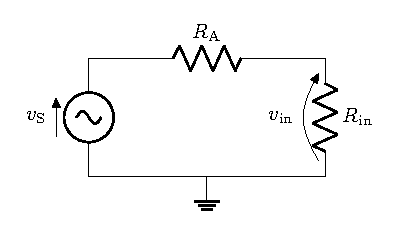
\includegraphics{assets/antenna_equivalent_circuit.eps}
					\begin{circuitikz}[transform shape]
	\draw (0,0) to [sV=$v_{\mathrm{S}}$] (0,2);
	\draw (0,2) to [short] (1,2);
	\draw (1,2) to [R=$R_{\mathrm{A}}$] (3,2);
	\draw (3,2) to [short] (4,2);
	\draw (4,2) to [R=$R_{\mathrm{in}}$, v<=$v_{\mathrm{in}}$] (4,0);
	\draw (4,0) to [short] (2,0) node[ground](GND){};
	\draw (2,0) to [short] (0,0);
\end{circuitikz}

				}
			}
			\subfloat[A single diode rectifier\label{fi:single_diode_rectifier}]{
				\resizebox{0.45\columnwidth}{!}{
					% 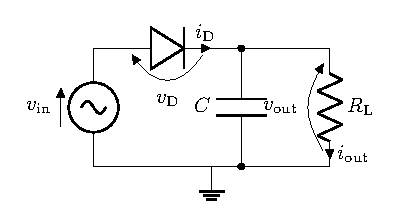
\includegraphics{assets/a_single_diode_rectifier.eps}
					\begin{circuitikz}[transform shape]
	\draw (0,0) to [sV=$v_{\mathrm{in}}$] (0,2);
	\draw (0,2) to [short] (0.25,2);
	\draw (0.25,2) to [D, v<=$v_{\mathrm{D}}$, i=$i_{\mathrm{D}}$] (2.25,2);
	\draw (2.25,2) to [short, -*] (2.5,2);
	\draw (2.5,2) to [C, l_=$C$, -*] (2.5,0);
	\draw (2.5,2) to [short] (4,2);
	\draw (4,2) to [R=$R_{\mathrm{L}}$, v<=$v_{\mathrm{out}}$, i=$i_{\mathrm{out}}$] (4,0);
	\draw (4,0) to [short] (2,0) node[ground](GND){};
	\draw (2,0) to [short] (0,0);
\end{circuitikz}

				}
			}
			\caption{Equivalent circuits of receive antenna and energy harvester.}
		\end{figure}

		Taken from \cite{Clerckx2016a}, the rectenna model used in this section captures the dependency of the output \gls{dc} on both the power and shape of the received signal. Fig.~\subref*{fi:antenna_equivalent_circuit} illustrates the equivalent circuit of an ideal antenna, where the antenna has a resistance $R_{\mathrm{A}}$ and the incoming signal creates a voltage source $v_{\mathrm{S}}(t)$. Let $R_{\mathrm{in}}$ be the total input resistance of the rectifier and matching network, and we assume the voltage across the matching network is negligible. When perfectly matched (i.e., $R_{\mathrm{in}}=R_{\mathrm{A}}$), the rectifier input voltage is $v_{\mathrm{in}}(t)=y(t)\sqrt{\rho R_{\mathrm{A}}}$. Consider a simplified rectifier model in Fig.~\subref*{fi:single_diode_rectifier} where a single series diode is followed by a low-pass filter with a parallel load. As detailed in \cite{Clerckx2018b}, a truncated Taylor expansion of the diode I-V characteristic equation suggests that maximizing the average output \gls{dc} is equivalent to maximizing a monotonic function\footnote{This small-signal expansion model is only valid for the nonlinear operation region of the diode, and the I-V relationship would be linear if the diode behavior is dominated by the load \cite{Clerckx2016a}.}
		\begin{equation}\label{eq:z}
			z(\boldsymbol{\phi},\boldsymbol{w}_{\mathrm{I}},\boldsymbol{w}_{\mathrm{P}},\rho)=\sum_{i\,\mathrm{even},i\ge2}^{n_0}{k_i}{\rho^{i/2}}{R_{\mathrm{A}}^{i/2}}{\mathbb{E}\left\{\mathbb{A}\left\{y(t)^i\right\}\right\}},
		\end{equation}
		where $n_0$ is the truncation order and $k_i \triangleq i_{\mathrm{S}}/i!(n'v_{\mathrm{T}})^i$ is the diode coefficient ($i_{\mathrm{S}}$ is the reverse bias saturation current, $n'$ is the diode ideality factor, $v_{\mathrm{T}}$ is the thermal voltage). With a slight abuse of notation, we refer to $z$ as the average output \gls{dc} in this paper. It can be observed that the conventional linear harvester model, where the output \gls{dc} power equals the sum of the power harvested on each frequency, is a special case of \eqref{eq:z} with $n_0=2$. However, due to the coupling effect among different frequencies, some high-order frequency components compensate each other in frequency and further contribute to the output \gls{dc} power. In other words, even-order terms with $i \ge 4$ account for the nonlinear diode behavior. For simplicity, we choose $n_0=4$ to investigate the fundamental rectifier nonlinearity, and define $\beta_2 \triangleq {k_2}{R_{\mathrm{A}}}$, $\beta_4 \triangleq {k_4}{R_{\mathrm{A}}^2}$ to rewrite $z$ by \eqref{eq:z_expand}. Note that $\mathbb{E}\left\{\lvert\tilde{x}_{\mathrm{I},n}\rvert^2\right\}=1$ but $\mathbb{E}\left\{\lvert\tilde{x}_{\mathrm{I},n}\rvert^4\right\}=2$ applies a modulation gain on the fourth-order \gls{dc} terms. Let $\boldsymbol{W}_{\mathrm{I/P}} \triangleq \boldsymbol{w}_{\mathrm{I/P}}\boldsymbol{w}_{\mathrm{I/P}}^H \in \mathbb{C}^{MN \times MN}$. As illustrated by Fig.~\ref{fi:block_diagonal}, $\boldsymbol{W}_{\mathrm{I/P}}$ can be divided into $N \times N$ blocks of size $M \times M$, and we let $\boldsymbol{W}_{\mathrm{I/P},k}$ keep its block diagonal $k \in \{-N+1,\dots,N-1\}$ and set all other blocks to $\boldsymbol{0}$. Hence, the components of $z$ reduce to \eqref{eq:y_I2}--\eqref{eq:y_P4} \cite{Golub2013}.

		\begin{figure*}[!t]
			\begin{equation*}
				\boldsymbol{W}_{\mathrm{I/P}}=
				\begin{tikzpicture}[>=stealth,thick,baseline,every right delimiter/.append style={name=rd},]
					\matrix [matrix of math nodes,left delimiter=(,right delimiter=)] (m)
					{
						\boldsymbol{w}_{\mathrm{I/P},1}\boldsymbol{w}_{\mathrm{I/P},1}^H & \boldsymbol{w}_{\mathrm{I/P},1}\boldsymbol{w}_{\mathrm{I/P},2}^H & \dots & \boldsymbol{w}_{\mathrm{I/P},1}\boldsymbol{w}_{\mathrm{I/P},N}^H \\
						\boldsymbol{w}_{\mathrm{I/P},2}\boldsymbol{w}_{\mathrm{I/P},1}^H & \boldsymbol{w}_{\mathrm{I/P},2}\boldsymbol{w}_{\mathrm{I/P},2}^H & \ddots & \vdots \\
						\vdots & \ddots & \ddots & \boldsymbol{w}_{\mathrm{I/P},N-1}\boldsymbol{w}_{\mathrm{I/P},N}^H \\
						\boldsymbol{w}_{\mathrm{I/P},N}\boldsymbol{w}_{\mathrm{I/P},1}^H & \dots & \boldsymbol{w}_{\mathrm{I/P},N}\boldsymbol{w}_{\mathrm{I/P},N-1}^H & \boldsymbol{w}_{\mathrm{I/P},N}\boldsymbol{w}_{\mathrm{I/P},N}^H \\
					};
					\draw[dotted,thick] (m-4-1.north west) rectangle (m-4-1.south east);
					\draw[dotted,thick,fill=gray,opacity=0.125] (m-2-1.north west) rectangle (m-2-1.south east); \draw[dotted,thick,fill=gray,opacity=0.125] (m-3-2.north west) rectangle (m-3-2.south east); \draw[dotted,thick,fill=gray,opacity=0.125] (m-4-3.north west) rectangle (m-4-3.south east);
					\draw[dashed,thick,fill=gray,opacity=0.5] (m-1-1.north west) rectangle (m-1-1.south east); \draw[dashed,thick,fill=gray,opacity=0.5] (m-2-2.north west) rectangle (m-2-2.south east); \draw[dashed,thick,fill=gray,opacity=0.5] (m-3-3.north west) rectangle (m-3-3.south east); \draw[dashed,thick,fill=gray,opacity=0.5] (m-4-4.north west) rectangle (m-4-4.south east);
					\draw[solid,thick,fill=gray,opacity=0.25] (m-1-2.north west) rectangle (m-1-2.south east); \draw[solid,thick,fill=gray,opacity=0.25] (m-2-3.north west) rectangle (m-2-3.south east); \draw[solid,thick,fill=gray,opacity=0.25] (m-3-4.north west) rectangle (m-3-4.south east);
					\draw[solid,thick] (m-1-4.north west) rectangle (m-1-4.south east);
					\draw[<-] (m-4-3.south|-m.south) -- ++(0.5,-0.15) node[below]{$k=-1$};
					\draw[<-] (rd.east|-m.south) -- ++(0.5,-0.15) node[right]{$k=0$};
					\draw[<-] (rd.east|-m-3-4.east) -- ++(0.5,-0.15) node[right]{$k=1$};
				\end{tikzpicture}
			\end{equation*}
			\caption{$\boldsymbol{W}_{\mathrm{I/P}}$ consists of $N \times N$ blocks of size $M \times M$. $\boldsymbol{W}_{\mathrm{I/P},k}$ keeps the $k$-th block diagonal of $\boldsymbol{W}_{\mathrm{I/P}}$ and nulls all remaining blocks. Solid, dashed and dotted blocks correspond to $k>0$, $k=0$ and $k<0$, respectively. For $\boldsymbol{w}_{\mathrm{I/P},n_1}\boldsymbol{w}_{\mathrm{I/P},n_2}^H$, the $k$-th block diagonal satisfies $k=n_2-n_1$.}
			\label{fi:block_diagonal}
		\end{figure*}

		\begin{figure*}[!b]
			\hrule
			\begin{align}
				&z(\boldsymbol{\phi},\boldsymbol{w}_{\mathrm{I}},\boldsymbol{w}_{\mathrm{P}},\rho) = \beta_2\rho\Bigl(\mathbb{E}\left\{\mathbb{A}\left\{y_{\mathrm{I}}^2(t)\right\}\right\}+\mathbb{A}\left\{y_{\mathrm{P}}^2(t)\right\}\Bigr)+\beta_4\rho^2\Bigl(\mathbb{E}\left\{\mathbb{A}\left\{y_{\mathrm{I}}^4(t)\right\}\right\}+\mathbb{A}\left\{y_{\mathrm{P}}^4(t)\right\}+6\mathbb{E}\left\{\mathbb{A}\left\{y_{\mathrm{I}}^2(t)\right\}\right\}\mathbb{A}\left\{y_{\mathrm{P}}^2(t)\right\}\Bigr),\label{eq:z_expand}\\
				&\mathbb{E}\left\{\mathbb{A}\left\{y_{\mathrm{I}}^2(t)\right\}\right\} = \frac{1}{2}\sum_{n=1}^N{(\boldsymbol{h}_{n}^H\boldsymbol{w}_{\mathrm{I},n})(\boldsymbol{h}_{n}^H\boldsymbol{w}_{\mathrm{I},n})^*} = \frac{1}{2}\boldsymbol{h}^H\boldsymbol{W}_{\mathrm{I},0}\boldsymbol{h},\label{eq:y_I2}\\
				&\mathbb{E}\left\{\mathbb{A}\left\{y_{\mathrm{I}}^4(t)\right\}\right\} = \frac{3}{4}\left(\sum_{n=1}^N{(\boldsymbol{h}_{n}^H\boldsymbol{w}_{\mathrm{I},n})(\boldsymbol{h}_{n}^H\boldsymbol{w}_{\mathrm{I},n})^*}\right)^2 = \frac{3}{4}(\boldsymbol{h}^H\boldsymbol{W}_{\mathrm{I},0}\boldsymbol{h})^2,\label{eq:y_I4}\\
				&\mathbb{A}\left\{y_{\mathrm{P}}^2(t)\right\} = \frac{1}{2}\sum_{n=1}^N{(\boldsymbol{h}_{n}^H\boldsymbol{w}_{\mathrm{P},n})(\boldsymbol{h}_{n}^H\boldsymbol{w}_{\mathrm{P},n})^*} = \frac{1}{2}\boldsymbol{h}^H\boldsymbol{W}_{\mathrm{P},0}\boldsymbol{h},\label{eq:y_P2}\\
				&\mathbb{A}\left\{y_{\mathrm{P}}^4(t)\right\} = \frac{3}{8}\sum_{\substack{{n_1},{n_2},{n_3},{n_4}\\{n_1}+{n_2}={n_3}+{n_4}}}{(\boldsymbol{h}_{{n_1}}^H\boldsymbol{w}_{\mathrm{P},{n_1}})(\boldsymbol{h}_{{n_2}}^H\boldsymbol{w}_{\mathrm{P},{n_2}})(\boldsymbol{h}_{{n_3}}^H\boldsymbol{w}_{\mathrm{P},{n_3}})^*(\boldsymbol{h}_{{n_4}}^H\boldsymbol{w}_{\mathrm{P},{n_4}})^*} = \frac{3}{8}\sum_{k=-N+1}^{N-1}(\boldsymbol{h}^H\boldsymbol{W}_{\mathrm{P},k}\boldsymbol{h})(\boldsymbol{h}^H\boldsymbol{W}_{\mathrm{P},k}\boldsymbol{h})^*.\label{eq:y_P4}
			\end{align}
		\end{figure*}
	\end{subsection}


	\begin{subsection}{Rate-Energy Region}
		The achievable \gls{r-e} region is defined as
		\begin{align}
			\mathcal{C}_{\mathrm{\gls{r-e}}}
			&\triangleq \biggl\{(R_{\mathrm{ID}}, z_{\mathrm{EH}}) \in \mathbb{R}_+^2 \mid R_{\mathrm{ID}} \le R, z_{\mathrm{EH}} \le z,\nonumber\\
			&\quad \frac{1}{2}\left(\lVert{\boldsymbol{w}_{\mathrm{I}}}\rVert^2+\lVert{\boldsymbol{w}_{\mathrm{P}}}\rVert^2\right) \le P\biggr\},
		\end{align}
		where $P$ is the average transmit power budget and 1/2 converts the peak value of the sine waves to the average value.
	\end{subsection}
\end{section}


\begin{section}{Problem Formulation}\label{se:problem_formulation}
	We characterize each \gls{r-e} boundary point through a current maximization problem subject to sum rate, transmit power, and reflection amplitude constraints as
	\begin{maxi!}
		{\scriptstyle{\boldsymbol{\phi},\boldsymbol{w}_{\mathrm{I}},\boldsymbol{w}_{\mathrm{P}},\rho}}{z(\boldsymbol{\phi},\boldsymbol{w}_{\mathrm{I}},\boldsymbol{w}_{\mathrm{P}},\rho)}{\label{op:original}}{\label{ob:original}}
		\addConstraint{R(\boldsymbol{\phi},\boldsymbol{w}_{\mathrm{I}},\rho) \ge \bar{R}}\label{co:original_rate}
		\addConstraint{\frac{1}{2}\left(\lVert{\boldsymbol{w}_{\mathrm{I}}}\rVert^2+\lVert{\boldsymbol{w}_{\mathrm{P}}}\rVert^2\right)\le{P}}\label{co:original_power}
		\addConstraint{\lvert{\boldsymbol{\phi}}\rvert=\boldsymbol{1}}\label{co:original_modulus}
		\addConstraint{0 \le \rho \le 1.}
	\end{maxi!}
	Problem~\eqref{op:original} is intricate because of the coupled variables in \eqref{ob:original}, \eqref{co:original_rate} and the non-convex constraint \eqref{co:original_modulus}. To obtain a feasible solution, we propose a \gls{bcd} algorithm that iteratively updates (i) the \gls{ris} phase shift; (ii) the active precoder; (iii) the waveform amplitude and splitting ratio, until convergence.


	\begin{subsection}{Passive Beamforming}
		In this section, we optimize the \gls{ris} phase shift $\boldsymbol{\phi}$ for any given waveform $\boldsymbol{w}_{\mathrm{I/P}}$ and splitting ratio $\rho$. Note that
		\begin{align}
			\lvert \boldsymbol{h}_{n}^H\boldsymbol{w}_{\mathrm{I},n} \rvert^2
			& = \boldsymbol{w}_{a\mathrm{I},n}^H\boldsymbol{h}_n\boldsymbol{h}_n^H\boldsymbol{w}_{\mathrm{I},n}\nonumber\\
			& = \boldsymbol{w}_{\mathrm{I},n}^H(\boldsymbol{h}_{\mathrm{D},n}+\boldsymbol{V}_n^H\boldsymbol{\phi})(\boldsymbol{h}_{\mathrm{D},n}^H+\boldsymbol{\phi}^H\boldsymbol{V}_n)\boldsymbol{w}_{\mathrm{I},n}\nonumber\\
			& = \boldsymbol{w}_{\mathrm{I},n}^H\boldsymbol{M}_n^H\boldsymbol{\Phi}\boldsymbol{M}_n\boldsymbol{w}_{\mathrm{I},n}\nonumber\\
			& = \mathrm{tr}(\boldsymbol{M}_n\boldsymbol{w}_{\mathrm{I},n}\boldsymbol{w}_{\mathrm{I},n}^H\boldsymbol{M}_n^H\boldsymbol{\Phi})\nonumber\\
			& = \mathrm{tr}(\boldsymbol{C}_n\boldsymbol{\Phi}),
		\end{align}
		where $\boldsymbol{M}_n \triangleq [\boldsymbol{V}_n^H, \boldsymbol{h}_{\mathrm{D},n}]^H \in \mathbb{C}^{(L+1) \times M}$, $t'$ is an auxiliary variable with unit modulus, $\bar{\boldsymbol{\phi}} \triangleq [\boldsymbol{\phi}^H, t']^H \in \mathbb{C}^{(L+1) \times 1}$, $\boldsymbol{\Phi} \triangleq \bar{\boldsymbol{\phi}}\bar{\boldsymbol{\phi}}^H \in \mathbb{C}^{(L+1) \times (L+1)}$, $\boldsymbol{C}_n \triangleq \boldsymbol{M}_n\boldsymbol{w}_{\mathrm{I},n}\boldsymbol{w}_{\mathrm{I},n}^H\boldsymbol{M}_n^H \in \mathbb{C}^{(L+1)\times(L+1)}$. On the other hand, we define $t_{\mathrm{I/P},k}$ as
		\begin{align}
			t_{\mathrm{I/P},k}
			& \triangleq \boldsymbol{h}^H\boldsymbol{W}_{\mathrm{I/P},k}\boldsymbol{h}\nonumber\\
			& = \mathrm{tr}(\boldsymbol{h}\boldsymbol{h}^H\boldsymbol{W}_{\mathrm{I/P},k})\nonumber\\
			& = \mathrm{tr}\left((\boldsymbol{h}_{D}+\boldsymbol{V}^H\boldsymbol{\phi})(\boldsymbol{h}_{D}^H+\boldsymbol{\phi}^H\boldsymbol{V})\boldsymbol{W}_{\mathrm{I/P},k}\right)\nonumber\\
			& = \mathrm{tr}(\boldsymbol{M}^H\boldsymbol{\Phi}\boldsymbol{M}\boldsymbol{W}_{\mathrm{I/P},k})\nonumber\\
			& = \mathrm{tr}(\boldsymbol{M}\boldsymbol{W}_{\mathrm{I/P},k}\boldsymbol{M}^H\boldsymbol{\Phi})\nonumber\\
			& = \mathrm{tr}(\boldsymbol{C}_{\mathrm{I/P},k}\boldsymbol{\Phi})\label{eq:t_k},
		\end{align}
		where $\boldsymbol{V} \triangleq [\boldsymbol{V}_1,\dots,\boldsymbol{V}_N] \in \mathbb{C}^{L \times MN}$, $\boldsymbol{M} \triangleq [\boldsymbol{V}^H, \boldsymbol{h}_{D}]^H \in \mathbb{C}^{(L+1) \times MN}$, $\boldsymbol{C}_{\mathrm{I/P},k} \triangleq \boldsymbol{M}\boldsymbol{W}_{\mathrm{I/P},k}\boldsymbol{M}^H \in \mathbb{C}^{(L+1)\times(L+1)}$. On top of this, \eqref{eq:R} and \eqref{eq:z_expand} reduce respectively to
		\begin{align}
			R(\boldsymbol{\Phi})
			& = \sum_{n=1}^{N}{\log_2\left(1+\frac{(1-\rho)\mathrm{tr}(\boldsymbol{C}_n\boldsymbol{\Phi})}{\sigma_n^2}\right)},\label{eq:R_irs}\\
			z(\boldsymbol{\Phi})
			& = \frac{1}{2}{\beta_2}{\rho}(t_{\mathrm{I},0}+t_{\mathrm{P},0}) + \frac{3}{8}{\beta_4}{\rho^2} \left(2t_{\mathrm{I},0}^2 + \sum_{k=-N+1}^{N-1}{t_{\mathrm{P},k}t_{\mathrm{P},k}^*}\right)\nonumber\\
			& \quad + \frac{3}{2}{\beta_4}{\rho^2}t_{\mathrm{I},0}t_{\mathrm{P},0}.\label{eq:z_irs}
		\end{align}
		To maximize the non-concave expression \eqref{eq:z_irs}, we successively lower bound the second-order terms by their first-order Taylor expansions \cite{Adali2010}. Based on the solution at iteration $i - 1$, the approximations at iteration $i$ are
		\begin{align}
			(t_{\mathrm{I},0}^{(i)})^2
			& \ge 2 t_{\mathrm{I},0}^{(i)}t_{\mathrm{I},0}^{(i-1)} - (t_{\mathrm{I},0}^{(i-1)})^2,\label{eq:taylor_1}\\
			t_{\mathrm{P},k}^{(i)} (t_{\mathrm{P},k}^{(i)})^*
			& \ge 2 \Re\left\{t_{\mathrm{P},k}^{(i)} (t_{\mathrm{P},k}^{(i-1)})^*\right\} - t_{\mathrm{P},k}^{(i-1)} (t_{\mathrm{P},k}^{(i-1)})^*,\label{eq:taylor_2}\\
			t_{\mathrm{I},0}^{(i)} t_{\mathrm{P},0}^{(i)}
			& \ge t_{\mathrm{I},0}^{(i)} t_{\mathrm{P},0}^{(i-1)} + t_{\mathrm{P},0}^{(i)} t_{\mathrm{I},0}^{(i-1)} - t_{\mathrm{I},0}^{(i-1)} t_{\mathrm{P},0}^{(i-1)}.\label{eq:taylor_3}
		\end{align}
		Note that $t_{\mathrm{I/P},0}=\mathrm{tr}(\boldsymbol{C}_{\mathrm{I/P},0}\boldsymbol{\Phi})$ is real-valued because $\boldsymbol{C}_{\mathrm{I/P},0}$ and $\boldsymbol{\Phi}$ are Hermitian matrices. Due to symmetry \cite{Golub2013}, we have
		\begin{equation}\label{eq:coupled_terms}
			\sum_{k=-N+1}^{N-1} \Re\left\{t_{\mathrm{P},k}^{(i)} (t_{\mathrm{P},k}^{(i-1)})^*\right\} = \sum_{k=-N+1}^{N-1} t_{\mathrm{P},k}^{(i)} (t_{\mathrm{P},k}^{(i-1)})^*.
		\end{equation}
		Plugging \eqref{eq:taylor_1}--\eqref{eq:coupled_terms} into \eqref{eq:z_irs}, we obtain the \gls{dc} approximation $\tilde{z}$ as \eqref{eq:z_irs_approx} and transform problem~\eqref{op:original} to
		\begin{figure*}[!b]
			\hrule
			\begin{align}
				\tilde{z}(\boldsymbol{\Phi}^{(i)})
				& = \frac{1}{2}{\beta_2}{\rho}(t_{\mathrm{I},0}^{(i)}+t_{\mathrm{P},0}^{(i)}) + \frac{3}{8}{\beta_4}{\rho^2} \left(4 t_{\mathrm{I},0}^{(i)}t_{\mathrm{I},0}^{(i-1)} - 2 (t_{\mathrm{I},0}^{(i-1)})^2 + \sum_{k=-N+1}^{N-1}{2 t_{\mathrm{P},k}^{(i)} (t_{\mathrm{P},k}^{(i-1)})^* - t_{\mathrm{P},k}^{(i-1)} (t_{\mathrm{P},k}^{(i-1)})^*}\right)\nonumber\\
				& \quad + \frac{3}{2}{\beta_4}{\rho^2} \left(t_{\mathrm{I},0}^{(i)} t_{\mathrm{P},0}^{(i-1)} + t_{\mathrm{P},0}^{(i)} t_{\mathrm{I},0}^{(i-1)} - t_{\mathrm{I},0}^{(i-1)} t_{\mathrm{P},0}^{(i-1)}\right).\label{eq:z_irs_approx}
			\end{align}
		\end{figure*}
		\begin{maxi!}
			{\scriptstyle{\boldsymbol{\Phi}}}{\tilde{z}(\boldsymbol{\Phi})}{\label{op:irs}}{\label{ob:irs}}
			\addConstraint{R(\boldsymbol{\Phi}) \ge \bar{R}}\label{co:irs_rate}
			\addConstraint{\mathrm{diag}^{-1}(\boldsymbol{\Phi})=\boldsymbol{1}}\label{co:irs_modulus}
			\addConstraint{\boldsymbol{\Phi}\succeq{\boldsymbol{0}}}\label{co:irs_sd}
			\addConstraint{\mathrm{rank}(\boldsymbol{\Phi})=1.\label{co:irs_rank}}
		\end{maxi!}
		We then apply \gls{sdr} to the unit-rank constraint \eqref{co:irs_rank} and formulate a \gls{sdp} with approximation accuracy no greater than $\pi/4$ \cite{Luo2010b}. In this specific case, we found the solution provided by \texttt{CVX toolbox} \cite{Grant2016} to \eqref{ob:irs}-\eqref{co:irs_sd} is always rank-\num{1}. This conclusion is summarized below.

		\begin{proposition}\label{pr:relaxation}
			Any optimal solution $\boldsymbol{\Phi}^\star$ to the relaxed passive beamforming problem~\eqref{ob:irs}--\eqref{co:irs_sd} is rank-\num{1} such that \eqref{co:irs_rank} is tight and no loss is introduced by \gls{sdr}.
		\end{proposition}

		\begin{proof}\label{pf:relaxation}
			Please refer to Appendix~\ref{ap:relaxation}.
		\end{proof}

		In summary, we update $\boldsymbol{\Phi}^{(i)}$ until convergence, extract $\hat{\boldsymbol{\phi}}^\star$ by eigen decomposition, and retrieve the	\gls{ris} vector by $\boldsymbol{\phi}^{\star}=e^{j \arg\left([\hat{\boldsymbol{\phi}}^\star]_{(1:L)} \middle/ [\hat{\boldsymbol{\phi}}^\star]_{(L+1)}\right)}$. The passive beamforming design is summarized in the \gls{sca} Algorithm~\ref{al:sca}, where the relaxed problem \eqref{ob:irs}--\eqref{co:irs_sd} involves a $(L+1)$-order positive semi-definite matrix variable and $(L+2)$ linear constraints. Given a solution accuracy $\epsilon_{\mathrm{IPM}}$ for the interior-point method, the computational complexity of Algorithm~\ref{al:sca} is $\mathcal{O}\left(I_{\mathrm{\gls{sca}}}(L+2)^4 (L+1)^{0.5} \log(\epsilon_{\mathrm{IPM}}^{-1})\right)$, where $I_{\mathrm{\gls{sca}}}$ denotes the number of \gls{sca} iterations \cite{Luo2010b}.

		\begin{algorithm}[!t]
			\caption{\gls{sca}: \gls{ris} Phase Shift.}
			\label{al:sca}
			\begin{algorithmic}[1]
				\State \textbf{Input} $\beta_2$, $\beta_4$, $\boldsymbol{h}_{\mathrm{D},n}$, $\boldsymbol{V}_{n}$, $\sigma_n$, $\boldsymbol{w}_{\mathrm{I/P},n}$, $\rho$, $\bar{R}$, $\epsilon$, $\forall n$
				\State Construct $\boldsymbol{V}$, $\boldsymbol{M}$, $\boldsymbol{M}_n$, $\boldsymbol{C}_{n}$, $\boldsymbol{C}_{\mathrm{I/P},k}$, $\forall n,k$
				\State \textbf{Initialize} $i \gets 0$, $\boldsymbol{\Phi}^{(0)}$
				\State Set $t_{\mathrm{I/P},k}^{(0)}$, $\forall k$ by \eqref{eq:t_k}
				\State Compute $z^{(0)}$ by \eqref{eq:z_irs}
				\Repeat
					\State $i \gets i + 1$
					\State Get $\boldsymbol{\Phi}^{(i)}$ by solving \eqref{ob:irs}--\eqref{co:irs_sd}
					\State Update $t_{\mathrm{I/P},k}^{(i)}$, $\forall k$ by \eqref{eq:t_k}
					\State Compute $z^{(i)}$ by \eqref{eq:z_irs}
				\Until $\lvert z^{(i)}-z^{(i-1)} \rvert \le \epsilon$
				\State Set $\boldsymbol{\Phi}^{\star} \gets \boldsymbol{\Phi}^{(i)}$
				\State Get $\hat{\boldsymbol{\phi}}^\star$ by eigen decomposition, $\boldsymbol{\Phi}^{\star}=\hat{\boldsymbol{\phi}}^\star(\hat{\boldsymbol{\phi}}^\star)^H$
				\State Set $\boldsymbol{\phi}^{\star} \gets e^{j \arg\left([\hat{\boldsymbol{\phi}}^\star]_{(1:L)} \middle/ [\hat{\boldsymbol{\phi}}^\star]_{(L+1)}\right)}$
				\State \textbf{Output} $\boldsymbol{\phi}^{\star}$
			\end{algorithmic}
		\end{algorithm}

		\begin{proposition}\label{pr:sca}
			For any feasible initial point with given waveform and splitting ratio, the \gls{sca} Algorithm~\ref{al:sca} is guaranteed to converge to local optimal points of the original problem~\eqref{op:original}.
		\end{proposition}

		\begin{proof}\label{pf:sca}
			Please refer to Appendix~\ref{ap:sca}.
		\end{proof}
	\end{subsection}

	\begin{subsection}{Active Beamforming}
		The original waveform and active beamforming problem~\eqref{op:original} is over complex vectors $\boldsymbol{w}_{\mathrm{I/P}}$ of size $MN \times 1$. Next, we decouple the design in spatial and frequency domains, enable independent optimizations correspondingly, and reduce the size of variables from $2MN$ to $2(M+N)$. The weight on subband $n$ is essentially
		\begin{equation}\label{eq:w}
			\boldsymbol{w}_{\mathrm{I/P}, n} = s_{\mathrm{I/P}, n} \boldsymbol{b}_{\mathrm{I/P}, n},
		\end{equation}
		where $s_{\mathrm{I/P},n}$ denotes the amplitude of the modulated/multisine waveform at tone $n$, and $\boldsymbol{b}_{\mathrm{I/P}, n}$ denotes the corresponding information/power precoder. Define $\boldsymbol{s}_{\mathrm{I/P}} \triangleq [s_{\mathrm{I/P},1},\dots,s_{\mathrm{I/P},N}]^T \in \mathbb{R}_+^{N \times 1}$. The \gls{mrt} precoder at subband $n$ is given by
		\begin{equation}\label{eq:b_n}
			\boldsymbol{b}_{\mathrm{I/P}, n}^\star = \frac{\boldsymbol{h}_n}{\lVert{\boldsymbol{h}_n}\rVert}.
		\end{equation}

		\begin{proposition}\label{pr:mrt}
			For single-user \gls{swipt}, the global optimal information and power precoders coincide at the \gls{mrt}.
		\end{proposition}

		\begin{proof}\label{pf:mrt}
			Please refer to Appendix~\ref{ap:mrt}.
		\end{proof}
	\end{subsection}


	\begin{subsection}{Waveform and Splitting Ratio}
		Next, we jointly optimize the waveform amplitude $\boldsymbol{s}_{\mathrm{I/P}}$ and the splitting ratio $\rho$ for any given \gls{ris} phase shift $\boldsymbol{\phi}$ and active precoder $\boldsymbol{b}_{\mathrm{I/P},n}$, $\forall n$. On top of \eqref{eq:b_n}, the equivalent channel strength at subband $n$ is $\lVert{\boldsymbol{h}_n}\rVert$. Hence, the rate \eqref{eq:R} reduces to
		\begin{equation}\label{eq:R_waveform}
			R(\boldsymbol{s}_{\mathrm{I}},\rho) = \log_2\prod_{n=1}^N\left(1+\frac{(1-\rho)\lVert{\boldsymbol{h}_n}\rVert^2 s_{\mathrm{I},n}^2}{\sigma_n^2}\right),
		\end{equation}
		and the \gls{dc} \eqref{eq:z_expand} rewrites as \eqref{eq:z_waveform}, so that problem~\eqref{op:original} boils down to
		\begin{figure*}[!b]
			\hrule
			\begin{align}
				z(\boldsymbol{s}_{\mathrm{I}},\boldsymbol{s}_\mathrm{P},\rho)
				& = \frac{1}{2}{\beta_2}{\rho} \sum_{n=1}^N \lVert{\boldsymbol{h}_n}\rVert^2(s_{\mathrm{I},n}^2+s_{\mathrm{P},n}^2) + \frac{3}{8}{\beta_4}{\rho^2} \left( 2\sum_{n_1,n_2} \prod_{j=1}^2 \lVert{\boldsymbol{h}_{n_j}}\rVert^2 s_{\mathrm{I},{n_j}}^2 + \sum_{\substack{{n_1},{n_2},{n_3},{n_4}\\{n_1}+{n_2}={n_3}+{n_4}}} \prod_{j=1}^4 \lVert{\boldsymbol{h}_{n_j}}\rVert s_{\mathrm{P},{n_j}} \right)\nonumber\\
				& \quad + \frac{3}{2}{\beta_4}{\rho^2} \left( \sum_{n_1,n_2} \lVert{\boldsymbol{h}_{n_1}}\rVert^2 \lVert{\boldsymbol{h}_{n_2}}\rVert^2 s_{\mathrm{I},{n_1}}^2 s_{\mathrm{P},{n_2}}^2 \right).\label{eq:z_waveform}
			\end{align}
		\end{figure*}
		\begin{maxi!}
			{\scriptstyle{\boldsymbol{s}_{\mathrm{I}},\boldsymbol{s}_\mathrm{P},\rho}}{z(\boldsymbol{s}_{\mathrm{I}},\boldsymbol{s}_\mathrm{P},\rho)}{\label{op:waveform}}{}
			\addConstraint{R(\boldsymbol{s}_{\mathrm{I}},\rho) \ge \bar{R}}
			\addConstraint{\frac{1}{2}\left(\lVert{\boldsymbol{s}_{\mathrm{I}}}\rVert^2+\lVert{\boldsymbol{s}_\mathrm{P}}\rVert^2\right)\le{P}.}
		\end{maxi!}
		Following \cite{Clerckx2018b}, we introduce auxiliary variables $t'',\bar{\rho}$ and transform problem~\eqref{op:waveform} into a reversed \gls{gp}
		\begin{mini!}
			{\scriptstyle{\boldsymbol{s}_{\mathrm{I}},\boldsymbol{s}_\mathrm{P},\rho,\bar{\rho},t''}}{\frac{1}{t''}}{\label{op:waveform_rgp}}{}
			\addConstraint{\frac{t''}{z(\boldsymbol{s}_{\mathrm{I}},\boldsymbol{s}_\mathrm{P},\rho)} \le 1}\label{co:waveform_objective}
			\addConstraint{\frac{2^{\bar{R}}}{\prod_{n=1}^N \left(1+{\bar{\rho}\lVert{\boldsymbol{h}_n}\rVert^2 s_{\mathrm{I},n}^2}\big/{\sigma_n^2}\right)} \le 1}\label{co:waveform_rate}
			\addConstraint{\frac{1}{2}\left(\lVert{\boldsymbol{s}_{\mathrm{I}}}\rVert^2+\lVert{\boldsymbol{s}_\mathrm{P}}\rVert^2\right) \le P}\label{co:waveform_power}
			\addConstraint{\rho + \bar{\rho} \le 1.}\label{co:waveform_splitting_ratio}
		\end{mini!}
		It can be concluded that $\bar{\rho}^{\star}=1-\rho^{\star}$ as no power is wasted at the receiver. The denominators of \eqref{co:waveform_rate} and \eqref{co:waveform_objective} consist of posynomials \cite{Boyd2007} that can be decomposed as sums of monomials
		\begin{align}
			1+\frac{\bar{\rho}\lVert{\boldsymbol{h}_n}\rVert^2 s_{\mathrm{I},n}^2}{\sigma_n^2} &\triangleq \sum_{m_{\mathrm{I},n}}g_{m_{\mathrm{I},n}}(s_{\mathrm{I},n},\bar{\rho})\label{eq:g_I},\\
			z(\boldsymbol{s}_{\mathrm{I}},\boldsymbol{s}_\mathrm{P},\rho) &\triangleq \sum_{m_\mathrm{P}}{g_{m_\mathrm{P}}(\boldsymbol{s}_{\mathrm{I}},\boldsymbol{s}_\mathrm{P},\rho)}\label{eq:g_P}.
		\end{align}
		We upper bound \eqref{eq:g_I} and \eqref{eq:g_P} by the \gls{gm}-\gls{am} inequality \cite{Chiang2005} and transform problem~\eqref{op:waveform_rgp} to
		\begin{mini!}
			{\scriptstyle{\boldsymbol{s}_{\mathrm{I}},\boldsymbol{s}_\mathrm{P},\rho,\bar{\rho},t''}}{\frac{1}{t''}}{\label{op:waveform_gp}}{}
			\addConstraint{{t''}\prod_{m_\mathrm{P}}{\left(\frac{g_{{m_\mathrm{P}}}(\boldsymbol{s}_{\mathrm{I}},\boldsymbol{s}_\mathrm{P},\rho)}{\gamma_{{m_\mathrm{P}}}}\right)^{-\gamma_{{m_\mathrm{P}}}}}\le{1}}
			\addConstraint{2^{\bar{R}}\prod_{n}\prod_{m_{\mathrm{I},n}}\left(\frac{g_{m_{\mathrm{I},n}}(s_{\mathrm{I},n},\bar{\rho})}{\gamma_{m_{\mathrm{I},n}}}\right)^{-\gamma_{m_{\mathrm{I},n}}}\le{1}}
			\addConstraint{\frac{1}{2}\left(\lVert{\boldsymbol{s}_{\mathrm{I}}}\rVert^2+\lVert{\boldsymbol{s}_\mathrm{P}}\rVert^2\right)\le{P}}
			\addConstraint{\rho + \bar{\rho} \le 1,}
		\end{mini!}
		where $\gamma_{m_{\mathrm{I},n}},\gamma_{m_\mathrm{P}} \ge 0$ and $\sum_{m_{\mathrm{I},n}}\gamma_{m_{\mathrm{I},n}}=\sum_{m_\mathrm{P}}\gamma_{m_\mathrm{P}}=1$. The tightness of the AM-GM inequality depends on $\{\gamma_{m_{\mathrm{I},n}},\gamma_{m_\mathrm{P}}\}$, and a feasible choice at iteration $i$ is
		\begin{align}
			\gamma_{m_{\mathrm{I},n}}^{(i)} & = \frac{g_{m_{\mathrm{I},n}}(s_{\mathrm{I},n}^{(i-1)},\bar{\rho}^{(i-1)})}{1+{\bar{\rho}^{(i-1)}\lVert{\boldsymbol{h}_n}\rVert^2 (s_{\mathrm{I},n}^{(i-1)})^2}\big/{\sigma_n^2}}\label{eq:gamma_I},\\
			\gamma_{m_\mathrm{P}}^{(i)} & = \frac{g_{m_\mathrm{P}}(\boldsymbol{s}_{\mathrm{I}}^{(i-1)},\boldsymbol{s}_\mathrm{P}^{(i-1)},\rho^{(i-1)})}{z(\boldsymbol{s}_{\mathrm{I}}^{(i-1)},\boldsymbol{s}_\mathrm{P}^{(i-1)},\rho^{(i-1)})}\label{eq:gamma_P}.
		\end{align}
		With \eqref{eq:gamma_I} and \eqref{eq:gamma_P}, problem~\eqref{op:waveform_gp} can be solved by existing optimization tools such as \texttt{CVX toolbox} \cite{Grant2016}. We update $\boldsymbol{s}_{\mathrm{I}}^{(i)},\boldsymbol{s}_\mathrm{P}^{(i)},\rho^{(i)}$ iteratively until convergence. The joint waveform amplitude and splitting ratio design is summarized in the \gls{gp} Algorithm~\ref{al:gp}, which achieves local optimality at the cost of exponential computational complexity \cite{Chiang2005}.

		\begin{algorithm}[!t]
			\caption{\gls{gp}: Waveform Amplitude and Splitting Ratio.}
			\label{al:gp}
			\begin{algorithmic}[1]
				\State \textbf{Input} $\beta_2$, $\beta_4$, $\boldsymbol{h}_n$, $P$, $\sigma_n$, $\bar{R}$, $\epsilon$, $\forall n$
				\State \textbf{Initialize} $i \gets 0$, $\boldsymbol{s}_{\mathrm{I/P}}^{(0)}$, $\rho^{(0)}$
				\State Compute $R^{(0)}$, $z^{(0)}$ by \eqref{eq:R_waveform}, \eqref{eq:z_waveform}
				\State Set $g_{m_{\mathrm{I},n}}^{(0)}$, $g_{m_\mathrm{P}}^{(0)}$, $\forall n$ by \eqref{eq:g_I}, \eqref{eq:g_P}
				\Repeat
					\State $i \gets i + 1$
					\State Update $\gamma_{m_{\mathrm{I},n}}^{(i)}$, $\gamma_{m_\mathrm{P}}^{(i)}$, $\forall n$ by \eqref{eq:gamma_I}, \eqref{eq:gamma_P}
					\State Get $\boldsymbol{s}_{\mathrm{I/P}}^{(i)}$, $\rho^{(i)}$ by solving problem~\eqref{op:waveform_gp}
					\State Compute $R^{(i)}$, $z^{(i)}$ by \eqref{eq:R_waveform}, \eqref{eq:z_waveform}
					\State Update $g_{m_{\mathrm{I},n}}^{(i)}$, $g_{m_\mathrm{P}}^{(i)}$, $\forall n$ by \eqref{eq:g_I}, \eqref{eq:g_P}
				\Until $\lvert z^{(i)} - z^{(i-1)} \rvert \le \epsilon$
				\State Set $\boldsymbol{s}_{\mathrm{I/P}}^{\star} \gets \boldsymbol{s}_{\mathrm{I/P}}^{(i)}$, $\rho^{\star} \gets \rho^{(i)}$
				\State \textbf{Output} $\boldsymbol{s}_{\mathrm{I}}^{\star}$, $\boldsymbol{s}_{\mathrm{P}}^{\star}$, $\rho^{\star}$
			\end{algorithmic}
		\end{algorithm}

		\begin{proposition}\label{pr:gp}
			For any feasible initial point, the \gls{gp} Algorithm~\ref{al:gp} is guaranteed to converge to local optimal points of the waveform amplitude and splitting ratio design problem \eqref{op:waveform}.
		\end{proposition}

		\begin{proof}\label{pf:gp}
			Please refer to \cite{Clerckx2016a,Clerckx2018b}.
		\end{proof}
	\end{subsection}


	\begin{subsection}{Low-Complexity Adaptive Design}
		To facilitate practical \gls{swipt} implementation, we propose two closed-form adaptive waveform amplitude schemes by combining \gls{wf} and \gls{smf} in time and power domains, respectively. For \gls{wit}, the optimal \gls{wf} strategy assigns the amplitude of modulated tone $n$ by
		\begin{equation}\label{eq:wf}
			s_{\mathrm{I}, n} = \sqrt{2\left(\lambda - \frac{\sigma_n^2}{P \lVert{\boldsymbol{h}_n}\rVert^2}\right)^+},
		\end{equation}
		where $\lambda$ is chosen to satisfy the power constraint $\lVert{\boldsymbol{s}_I}\rVert^2 / 2 \le P$. The closed-form solution can be obtained by iterative power allocation \cite{Tse2005}, and the details are omitted here. On the other hand, \gls{smf} was proposed in \cite{Clerckx2017} as a suboptimal \gls{wpt} resource allocation scheme that assigns the amplitude of sinewave $n$ by
		\begin{equation}\label{eq:smf}
			s_{\mathrm{P}, n} = \sqrt{\frac{2 P}{\sum_{n=1}^N \lVert{\boldsymbol{h}_n \rVert^{2 \alpha}}}}\lVert{\boldsymbol{h}_n}\rVert^\alpha,
		\end{equation}
		where the scaling ratio $\alpha \ge 1$ is predetermined to exploit the rectifier nonlinearity and frequency selectivity. When the receiver works in \gls{ts} mode, there is no superposition in the suboptimal waveform design (modulated waveform with amplitude \eqref{eq:wf} is used in the data session while multisine waveform with amplitude \eqref{eq:smf} is used in the energy session). When the receiver works in \gls{ps} mode, we jointly design the combining ratio $\delta$ with the splitting ratio $\rho$, and assign the superposed waveform amplitudes as
		\begin{align}
			s_{\mathrm{I}, n} &= \sqrt{2(1 - \delta)\left(\lambda - \frac{\sigma_n^2}{P \lVert{\boldsymbol{h}_n}\rVert^2}\right)^+}, \label{eq:s_i}\\
			s_{\mathrm{P}, n} &= \sqrt{\frac{2 \delta P}{\sum_{n=1}^N \lVert{\boldsymbol{h}_n \rVert^{2 \alpha}}}}\lVert{\boldsymbol{h}_n}\rVert^\alpha, \label{eq:s_p}
		\end{align}
		where the $\delta$ determines the power ratio of multisine waveform at the transmitter, and $\rho$ determines the power ratio of the energy harvester at the receiver.\footnote{We notice that $\delta^{\star}=\rho^{\star}=0$ at the \gls{wit} point and $\delta^{\star}=\rho^{\star}=1$ at the \gls{wpt} point when $N$ is relatively large. Intuitively, $\delta^{\star}$ and $\rho^{\star}$ should be positively correlated for efficient \gls{swipt} design.}

		Besides, minor modifications are required for passive beamforming to accommodate the low-complexity waveform schemes. Specifically, the rate constraint \eqref{co:irs_rate} should be dropped as the achievable rate is controlled by $\eta$ or $\{\delta,\rho\}$. To achieve the \gls{wit} point ($\rho=0$), the rate \eqref{eq:R_irs} should be maximized, the current expression \eqref{eq:z_irs_approx} is not needed and no \gls{sca} is involved. The Modified-\gls{sca} (M-\gls{sca}) Algorithm~\ref{al:m_sca} summarizes the modified passive beamforming design when the receiver works in \gls{ps} mode. Similarly, no loss is introduced by \gls{sdr} and local optimality is guaranteed. The proofs are omitted here. Since each \gls{sdp} involves $(L+1)$ linear constraints, the computational complexity of Algorithm~\ref{al:m_sca} is $\mathcal{O}\left(I_{\mathrm{M-\gls{sca}}}(L+1)^{4.5} \log(\epsilon_{\mathrm{IPM}}^{-1})\right)$, where $I_{\mathrm{M-\gls{sca}}}$ denotes the number of M-\gls{sca} iterations \cite{Luo2010b}. Note that no \gls{sca} is involved at the \gls{wit} point where $I_{\mathrm{M-\gls{sca}}}=1$.

		\begin{algorithm}[!t]
			\caption{M-\gls{sca}: \gls{ris} Phase Shift.}
			\label{al:m_sca}
			\begin{algorithmic}[1]
				\State \textbf{Input} $\beta_2$, $\beta_4$, $\boldsymbol{h}_{\mathrm{D},n}$, $\boldsymbol{V}_{n}$, $\sigma_n$, $\boldsymbol{w}_{\mathrm{I/P},n}$, $\rho$, $\epsilon$, $\forall n$
				\State Construct $\boldsymbol{V}$, $\boldsymbol{M}$, $\boldsymbol{M}_n$, $\boldsymbol{C}_{n}$, $\boldsymbol{C}_{\mathrm{I/P},k}$, $\forall n,k$
				\State \textbf{Initialize} $i \gets 0$, $\boldsymbol{\Phi}^{(0)}$
				\If{$\rho=0$}
					\State Get $\boldsymbol{\Phi}^{\star}$ by maximizing \eqref{eq:R_irs} s.t. \eqref{co:irs_modulus}, \eqref{co:irs_sd}
				\Else
					\State Set $t_{\mathrm{I/P},k}^{(0)}$, $\forall k$ by \eqref{eq:t_k}
					\State Compute $z^{(0)}$ by \eqref{eq:z_irs}
					\Repeat
						\State $i \gets i + 1$
							\State Get $\boldsymbol{\Phi}^{(i)}$ by maximizing \eqref{eq:z_irs_approx} s.t. \eqref{co:irs_modulus}, \eqref{co:irs_sd}
							\State Update $t_{\mathrm{I/P},k}^{(i)}$, $\forall k$ by \eqref{eq:t_k}
							\State Compute $z^{(i)}$ by \eqref{eq:z_irs}
					\Until $\lvert z^{(i)}-z^{(i-1)} \rvert \le \epsilon$
					\State Set $\boldsymbol{\Phi}^{\star} \gets \boldsymbol{\Phi}^{(i)}$
				\EndIf
				\State Get $\hat{\boldsymbol{\phi}}^\star$ by eigen decomposition, $\boldsymbol{\Phi}^{\star}=\hat{\boldsymbol{\phi}}^\star(\hat{\boldsymbol{\phi}}^\star)^H$
				\State Set $\boldsymbol{\phi}^{\star} \gets e^{j \arg\left([\hat{\boldsymbol{\phi}}^\star]_{(1:L)} \middle/ [\hat{\boldsymbol{\phi}}^\star]_{(L+1)}\right)}$
				\State \textbf{Output} $\boldsymbol{\phi}^{\star}$
			\end{algorithmic}
		\end{algorithm}
	\end{subsection}


	\begin{subsection}{Block Coordinate Descent}
		Based on the direct and cascaded \gls{csit}, we iteratively update the passive beamforming $\boldsymbol{\phi}$ by Algorithm~\ref{al:sca}, the active precoder $\boldsymbol{b}_{\mathrm{I/P},n}$, $\forall n$ by equation \eqref{eq:b_n}, and the waveform amplitude $\boldsymbol{s}_{\mathrm{I/P}}$ and splitting ratio $\rho$ by Algorithm~\ref{al:gp}, until convergence. The steps are summarized in the \gls{bcd} Algorithm~\ref{al:bcd}, whose computational complexity is exponential as inherited from Algorithm~\ref{al:gp}. It is guaranteed to converge, but may end up with a suboptimal solution because variables are coupled in constraint~\eqref{co:original_rate} \cite{Grippo2000}.

		\begin{algorithm}[!t]
			\caption{\gls{bcd}: Waveform, Beamforming and Splitting Ratio.}
			\label{al:bcd}
			\begin{algorithmic}[1]
				\State \textbf{Input} $\beta_2$, $\beta_4$, $\boldsymbol{h}_{\mathrm{D},n}$, $\boldsymbol{V}_{n}$, $P$, $\sigma_n$, $\bar{R}$, $\epsilon$, $\forall n$
				\State \textbf{Initialize} $i \gets 0$, $\boldsymbol{\phi}^{(0)}$, $\boldsymbol{b}_{\mathrm{I/P},n}^{(0)}$, $\boldsymbol{s}_{\mathrm{I/P}}^{(0)}$, $\rho^{(0)}$, $\forall n$
				\State Set $\boldsymbol{w}_{\mathrm{I/P},n}^{(0)}$, $\forall n$ by \eqref{eq:w}
				\State Compute $z^{(0)}$ by \eqref{eq:z_waveform}
				\Repeat
					\State $i \gets i + 1$
					\State Get $\boldsymbol{\phi}^{(i)}$ based on $\boldsymbol{w}_{\mathrm{I/P}}^{(i-1)}$, $\rho^{(i-1)}$ by Algorithm~\ref{al:sca}
					\State Update $\boldsymbol{h}_n^{(i)}$, $\boldsymbol{b}_n^{(i)}$, $\forall n$ by \eqref{eq:h_n}, \eqref{eq:b_n}
					\State Get $\boldsymbol{s}_{\mathrm{I/P}}^{(i)}$, $\rho^{(i)}$ by Algorithm~\ref{al:gp}
					\State Update $\boldsymbol{w}_{\mathrm{I/P},n}^{(i)}$, $\forall n$ by \eqref{eq:w}
					\State Compute $z^{(i)}$ by \eqref{eq:z_waveform}
				\Until $\lvert z^{(i)} - z^{(i-1)} \rvert \le \epsilon$
				\State Set $\boldsymbol{\phi}^{\star} \gets \boldsymbol{\phi}^{(i)}$, $\boldsymbol{w}_{\mathrm{I/P}}^{\star} \gets \boldsymbol{w}_{\mathrm{I/P}}^{(i)}$, $\rho^{\star} \gets \rho^{(i)}$
				\State \textbf{Output} $\boldsymbol{\phi}^{\star}$, $\boldsymbol{w}_{\mathrm{I}}^{\star}$, $\boldsymbol{w}_{\mathrm{P}}^{\star}$, $\rho^{\star}$
			\end{algorithmic}
		\end{algorithm}

		For the low-complexity design under \gls{ps} mode, we obtain the phase shift by Algorithm~\ref{al:m_sca}, the active precoder $\boldsymbol{b}_{\mathrm{I/P},n}$, $\forall n$ by equation \eqref{eq:b_n}, and the waveform amplitude by \eqref{eq:s_i} and \eqref{eq:s_p}. To achieve the \gls{wit} point ($\rho=0$), the rate \eqref{eq:R_irs} should be maximized to obtain the maximum capacity $C_{\max}$.\footnote{Recall in Remark~\ref{re:subband_tradeoff} that different subchannel designs lead to different capacities.} Note that the \gls{bcd} algorithm obtains the \gls{r-e} region by varying the rate constraint from \num{0} to $C_{\max}$, while the achievable \gls{r-e} region of the \gls{lc}-\gls{bcd} algorithm can be obtained by performing a two-dimensional search over $(\delta, \rho)$ from $(0, 0)$ to $(1, 1)$. The steps are summarized in Algorithm~\ref{al:lc_bcd}. The computational complexity of Algorithm~\ref{al:lc_bcd} is $\mathcal{O}\left(I_{\mathrm{\gls{lc}-\gls{bcd}}}I_{\mathrm{M-\gls{sca}}}(L+1)^{4.5} \log(\epsilon_{\mathrm{IPM}}^{-1})\right)$, where $I_{\mathrm{\gls{lc}-\gls{bcd}}}$ denotes the number of \gls{lc}-\gls{bcd} iterations \cite{Luo2010b}.

		\begin{algorithm}[!t]
			\caption{\gls{lc}-\gls{bcd}: Waveform and Beamforming.}
			\label{al:lc_bcd}
			\begin{algorithmic}[1]
				\State \textbf{Input} $\beta_2$, $\beta_4$, $\boldsymbol{h}_{\mathrm{D},n}$, $\boldsymbol{V}_{n}$, $P$, $\sigma_n$, $\delta$, $\rho$, $\epsilon$, $\forall n$
				\State \textbf{Initialize} $i \gets 0$, $\boldsymbol{\phi}^{(0)}$, $\boldsymbol{b}_{\mathrm{I/P},n}^{(0)}$, $\boldsymbol{s}_{\mathrm{I/P}}^{(0)}$, $\forall n$
				\State Set $\boldsymbol{w}_{\mathrm{I/P},n}^{(0)}$, $\forall n$ by \eqref{eq:w}
				\State Compute $R^{(0)}$, $z^{(0)}$ by \eqref{eq:R_waveform}, \eqref{eq:z_waveform}
				\Repeat
					\State $i \gets i + 1$
					\State Get $\boldsymbol{\phi}^{(i)}$ based on $\boldsymbol{w}_{\mathrm{I/P}}^{(i-1)}$ by Algorithm~\ref{al:m_sca}
					\State Update $\boldsymbol{h}_n^{(i)}$, $\boldsymbol{b}_n^{(i)}$, $\forall n$ by \eqref{eq:h_n}, \eqref{eq:b_n}
					\State Update $\boldsymbol{s}_{\mathrm{I}}^{(i)}$, $\boldsymbol{s}_{\mathrm{P}}^{(i)}$ by \eqref{eq:s_i}, \eqref{eq:s_p}
					\State Update $\boldsymbol{w}_{\mathrm{I/P},n}^{(i)}$, $\forall n$ by \eqref{eq:w}
					\State Compute $R^{(i)}$, $z^{(i)}$ by \eqref{eq:R_waveform}, \eqref{eq:z_waveform}
					\If{$\rho=0$}
						\State $\Delta \gets R^{(i)} - R^{(i-1)}$
					\Else
						\State $\Delta \gets z^{(i)} - z^{(i-1)}$
					\EndIf
				\Until $\lvert \Delta \rvert \le \epsilon$
				\State Set $\boldsymbol{\phi}^{\star} \gets \boldsymbol{\phi}^{(i)}$, $\boldsymbol{w}_{\mathrm{I/P}}^{\star} \gets \boldsymbol{w}_{\mathrm{I/P}}^{(i)}$
				\State \textbf{Output} $\boldsymbol{\phi}^{\star}$, $\boldsymbol{w}_{\mathrm{I}}^{\star}$, $\boldsymbol{w}_{\mathrm{P}}^{\star}$
			\end{algorithmic}
		\end{algorithm}
	\end{subsection}
\end{section}


\begin{section}{Performance Evaluations}\label{se:performance_evaluation}
	\begin{figure}[!t]
		\centering
		\def\svgwidth{0.9\columnwidth}
		% \import{assets/}{layout.eps_tex}
		\input{assets/chapter_3/layout.eps_tex}
		\caption{System layout in simulation.}
		\label{fi:layout}
	\end{figure}

	To evaluate the proposed \gls{ris}-aided \gls{swipt} system, we consider the layout in Fig.~\ref{fi:layout} where the \gls{ris} moves along a line parallel to the \gls{ap}-\gls{ue} path. Let $d_{\mathrm{H}}$, $d_{\mathrm{V}}$ be the horizontal and vertical distances from the \gls{ap} to the \gls{ris}, and denote respectively $d_{\mathrm{D}}$, $d_{\mathrm{I}}=\sqrt{d_{\mathrm{H}}^2+d_{\mathrm{V}}^2}$, $d_{\mathrm{R}}=\sqrt{(d_{\mathrm{D}}-d_{\mathrm{H}})^2+d_{\mathrm{V}}^2}$ as the distance of direct, incident and reflected links. $d_{\mathrm{D}}=\qty{12}{\meter}$ and $d_{\mathrm{H}}=d_{\mathrm{V}}=\qty{2}{\meter}$ are chosen as reference. The path loss of direct, incident and reflected links are denoted by $\Lambda_{\mathrm{D}}$, $\Lambda_{\mathrm{I}}$ and $\Lambda_{\mathrm{R}}$, respectively. We consider a large open space Wi-Fi-like environment at center frequency \qty{2.4}{\GHz} where the channel follows IEEE TGn channel model D \cite{Erceg2004}. Specifically, the path loss exponent is \num{2} (i.e., free-space model) up to \qty{10}{\meter}, and \num{3.5} onwards to further penalize the channels with large distance. All fadings are modeled as \gls{nlos} with tap delays and powers specified in model D, and the tap gains are modeled as i.i.d. \gls{cscg} variables. Rectenna parameters are set to $k_2=0.0034$, $k_4=0.3829$, $R_{\mathrm{A}}=\qty{50}{\ohm}$ \cite{Clerckx2016a} such that $\beta_2=0.17$ and $\beta_4=957.25$. We also choose the average \gls{eirp} as $P=\qty{40}{dBm}$, the receive antenna gain as \qty{3}{dBi}, the scaling ratio as $\alpha=2$, and the tolerance as $\epsilon=10^{-8}$. To further reduce the complexity, we assume $\delta=\rho$ for simplicity and perform a one-dimensional search from \num{0} to \num{1} to obtain a inner \gls{r-e} bound for the \gls{lc}-\gls{bcd} algorithm. Each \gls{r-e} point is averaged over \num{200} channel realizations, and the $x$-axis is normalized to per-subband rate $R/N$.

	\begin{figure}[!t]
		\centering
		\resizebox{0.8\columnwidth}{!}{
			% 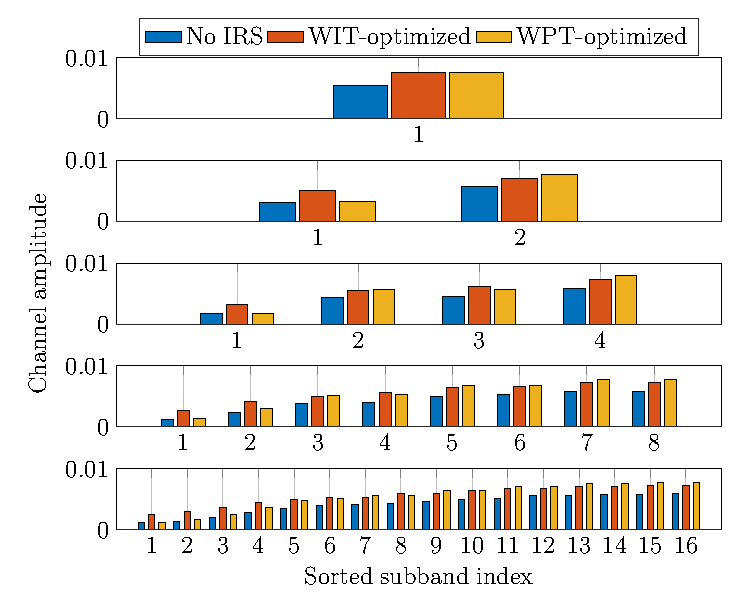
\includegraphics{assets/channel_amplitude.eps}
			% This file was created by matlab2tikz.
%
%The latest updates can be retrieved from
%  http://www.mathworks.com/matlabcentral/fileexchange/22022-matlab2tikz-matlab2tikz
%where you can also make suggestions and rate matlab2tikz.
%
\definecolor{mycolor1}{rgb}{0.00000,0.44700,0.74100}%
\definecolor{mycolor2}{rgb}{0.85000,0.32500,0.09800}%
\definecolor{mycolor3}{rgb}{0.92900,0.69400,0.12500}%
%
\begin{tikzpicture}[font=\footnotesize]

\begin{axis}[%
width=4.036in,
height=0.407in,
at={(0.677in,3.198in)},
scale only axis,
bar shift auto,
xmin=0,
xmax=2,
xtick={1},
ymin=0,
ymax=0.01,
ytick={   0, 0.01},
axis background/.style={fill=white},
xmajorgrids,
ymajorgrids,
legend style={at={(0.5,1.03)}, anchor=south, legend columns=3, legend cell align=left, align=left, draw=white!15!black},
scaled y ticks=false, yticklabel=\pgfkeys{/pgf/number format/.cd,fixed,precision=2}\pgfmathprintnumber{\tick}
]
\addplot[ybar, bar width=0.178, fill=mycolor1, draw=black, area legend] table[row sep=crcr] {%
1	0.00540099400856952\\
};
\addplot[forget plot, color=white!15!black] table[row sep=crcr] {%
0	0\\
2	0\\
};
\addlegendentry{No RIS}

\addplot[ybar, bar width=0.178, fill=mycolor2, draw=black, area legend] table[row sep=crcr] {%
1	0.00757609645318138\\
};
\addplot[forget plot, color=white!15!black] table[row sep=crcr] {%
0	0\\
2	0\\
};
\addlegendentry{WIT-optimized}

\addplot[ybar, bar width=0.178, fill=mycolor3, draw=black, area legend] table[row sep=crcr] {%
1	0.00757609644840316\\
};
\addplot[forget plot, color=white!15!black] table[row sep=crcr] {%
0	0\\
2	0\\
};
\addlegendentry{WPT-optimized}

\end{axis}

\begin{axis}[%
width=4.036in,
height=0.407in,
at={(0.677in,2.513in)},
scale only axis,
bar shift auto,
xmin=0,
xmax=3,
xtick={1, 2},
ymin=0,
ymax=0.01,
ytick={   0, 0.01},
axis background/.style={fill=white},
xmajorgrids,
ymajorgrids,
scaled y ticks=false, yticklabel=\pgfkeys{/pgf/number format/.cd,fixed,precision=2}\pgfmathprintnumber{\tick}
]
\addplot[ybar, bar width=0.178, fill=mycolor1, draw=black, area legend] table[row sep=crcr] {%
1	0.00314170999160457\\
2	0.00572485908105548\\
};
\addplot[forget plot, color=white!15!black] table[row sep=crcr] {%
0	0\\
3	0\\
};
\addplot[ybar, bar width=0.178, fill=mycolor2, draw=black, area legend] table[row sep=crcr] {%
1	0.00502314747430184\\
2	0.00698106265038798\\
};
\addplot[forget plot, color=white!15!black] table[row sep=crcr] {%
0	0\\
3	0\\
};
\addplot[ybar, bar width=0.178, fill=mycolor3, draw=black, area legend] table[row sep=crcr] {%
1	0.00330170889121358\\
2	0.00768466635770749\\
};
\addplot[forget plot, color=white!15!black] table[row sep=crcr] {%
0	0\\
3	0\\
};
\end{axis}

\begin{axis}[%
width=4.036in,
height=0.407in,
at={(0.677in,1.828in)},
scale only axis,
bar shift auto,
xmin=0,
xmax=5,
xtick={1, 2, 3, 4},
ymin=0,
ymax=0.01,
ytick={   0, 0.01},
ylabel style={font=\color{white!15!black}},
ylabel={Channel amplitude},
axis background/.style={fill=white},
xmajorgrids,
ymajorgrids,
scaled y ticks=false, yticklabel=\pgfkeys{/pgf/number format/.cd,fixed,precision=2}\pgfmathprintnumber{\tick}
]
\addplot[ybar, bar width=0.178, fill=mycolor1, draw=black, area legend] table[row sep=crcr] {%
1	0.0016696476908254\\
2	0.00438348129943761\\
3	0.00457133324563245\\
4	0.00586320993785494\\
};
\addplot[forget plot, color=white!15!black] table[row sep=crcr] {%
0	0\\
5	0\\
};
\addplot[ybar, bar width=0.178, fill=mycolor2, draw=black, area legend] table[row sep=crcr] {%
1	0.00326549483873511\\
2	0.00557307586676685\\
3	0.00614450761039544\\
4	0.00726164815517615\\
};
\addplot[forget plot, color=white!15!black] table[row sep=crcr] {%
0	0\\
5	0\\
};
\addplot[ybar, bar width=0.178, fill=mycolor3, draw=black, area legend] table[row sep=crcr] {%
1	0.00166671759288851\\
2	0.0056728199729895\\
3	0.00568370327308551\\
4	0.00789867646413342\\
};
\addplot[forget plot, color=white!15!black] table[row sep=crcr] {%
0	0\\
5	0\\
};
\end{axis}

\begin{axis}[%
width=4.036in,
height=0.407in,
at={(0.677in,1.143in)},
scale only axis,
bar shift auto,
xmin=0,
xmax=9,
xtick={1, 2, 3, 4, 5, 6, 7, 8},
ymin=0,
ymax=0.01,
ytick={   0, 0.01},
axis background/.style={fill=white},
xmajorgrids,
ymajorgrids,
scaled y ticks=false, yticklabel=\pgfkeys{/pgf/number format/.cd,fixed,precision=2}\pgfmathprintnumber{\tick}
]
\addplot[ybar, bar width=0.178, fill=mycolor1, draw=black, area legend] table[row sep=crcr] {%
1	0.00121164184157658\\
2	0.00238340383353008\\
3	0.00380683420957256\\
4	0.00397337725168322\\
5	0.00492524818026471\\
6	0.00528740868681232\\
7	0.00572071220385092\\
8	0.00587459497346489\\
};
\addplot[forget plot, color=white!15!black] table[row sep=crcr] {%
0	0\\
9	0\\
};
\addplot[ybar, bar width=0.178, fill=mycolor2, draw=black, area legend] table[row sep=crcr] {%
1	0.00264154779713112\\
2	0.00407667250014311\\
3	0.0049500895867949\\
4	0.00561010487339341\\
5	0.00637593781159189\\
6	0.0066081911104957\\
7	0.00719542472167268\\
8	0.00721447474714219\\
};
\addplot[forget plot, color=white!15!black] table[row sep=crcr] {%
0	0\\
9	0\\
};
\addplot[ybar, bar width=0.178, fill=mycolor3, draw=black, area legend] table[row sep=crcr] {%
1	0.00139675837927404\\
2	0.00297327122282322\\
3	0.00519768343232529\\
4	0.00524568965358895\\
5	0.00679027772006842\\
6	0.00680292145999757\\
7	0.00768611044981794\\
8	0.00771790378640739\\
};
\addplot[forget plot, color=white!15!black] table[row sep=crcr] {%
0	0\\
9	0\\
};
\end{axis}

\begin{axis}[%
width=4.036in,
height=0.407in,
at={(0.677in,0.458in)},
scale only axis,
bar shift auto,
xmin=0,
xmax=17,
xtick={ 1,  2,  3,  4,  5,  6,  7,  8,  9, 10, 11, 12, 13, 14, 15, 16},
xlabel style={font=\color{white!15!black}},
xlabel={Sorted subband index},
ymin=0,
ymax=0.01,
ytick={   0, 0.01},
axis background/.style={fill=white},
xmajorgrids,
ymajorgrids,
scaled y ticks=false, yticklabel=\pgfkeys{/pgf/number format/.cd,fixed,precision=2}\pgfmathprintnumber{\tick}
]
\addplot[ybar, bar width=0.178, fill=mycolor1, draw=black, area legend] table[row sep=crcr] {%
1	0.0011086419762005\\
2	0.00139817672195447\\
3	0.00200749223129634\\
4	0.00276896018192483\\
5	0.00348858569071252\\
6	0.00390863609607119\\
7	0.00410205684728188\\
8	0.00421746375099375\\
9	0.0046579451399174\\
10	0.00494987881895202\\
11	0.00517723522936086\\
12	0.00554845359626313\\
13	0.00558432983698075\\
14	0.00581133838542614\\
15	0.00582728083668895\\
16	0.00588378650142745\\
};
\addplot[forget plot, color=white!15!black] table[row sep=crcr] {%
0	0\\
17	0\\
};
\addplot[ybar, bar width=0.178, fill=mycolor2, draw=black, area legend] table[row sep=crcr] {%
1	0.00243240737767257\\
2	0.00291012490661641\\
3	0.00364483122694576\\
4	0.00450699183712641\\
5	0.00487492494056207\\
6	0.00519805292278296\\
7	0.00528263562038442\\
8	0.00589785004825321\\
9	0.0059831692545346\\
10	0.00639251285950617\\
11	0.00669911334288142\\
12	0.00680111371923813\\
13	0.00709923174422509\\
14	0.0071115147925566\\
15	0.00725582025143191\\
16	0.00726750007562416\\
};
\addplot[forget plot, color=white!15!black] table[row sep=crcr] {%
0	0\\
17	0\\
};
\addplot[ybar, bar width=0.178, fill=mycolor3, draw=black, area legend] table[row sep=crcr] {%
1	0.00123628236378877\\
2	0.00164057003125897\\
3	0.00244260991306404\\
4	0.00355854925167237\\
5	0.00469336613331463\\
6	0.00513906379517623\\
7	0.00552284927791181\\
8	0.00566659546513512\\
9	0.00636655282038687\\
10	0.0064643206674846\\
11	0.00710638804550398\\
12	0.00714275219594531\\
13	0.00755098826468563\\
14	0.00759919845334804\\
15	0.00776427719266845\\
16	0.00777739000911697\\
};
\addplot[forget plot, color=white!15!black] table[row sep=crcr] {%
0	0\\
17	0\\
};
\end{axis}
\end{tikzpicture}%

		}
		\caption{Sorted equivalent subchannel amplitude with and without \gls{ris} versus $N$ for $M=1$, $L=100$, $\sigma_n^2=\qty{-40}{dBm}$, $B=\qty{10}{\MHz}$ and $d_{\mathrm{H}}=d_{\mathrm{V}}=\qty{2}{\meter}$.}
		\label{fi:channel_amplitude}
	\end{figure}

	Fig.~\ref{fi:channel_amplitude} reveals how \gls{ris} influences the sorted equivalent subchannel amplitude for one channel realization. Due to the flexible subchannel design enabled by passive beamforming, the optimal amplitude distribution for \gls{wit} and \gls{wpt} are dissimilar. Under the specified configuration, the \gls{wpt}-optimized \gls{ris} aligns the strong subbands to exploit the rectifier nonlinearity. On the other hand, the \gls{wit}-optimized \gls{ris} provides a fair gain over all subchannels when $L$ is sufficiently large. This is reminiscent of the \gls{wf} scheme at high \gls{snr}, but is realized by channel alignment instead of resource allocation. Nevertheless, the amplitude of modulated and multisine waveforms remains approximately unchanged when adding a \gls{ris} (the plots are not attached). In other words, \gls{ris} has a subtle impact on the waveform design.

	\begin{figure}[!t]
		\centering
		\subfloat[\gls{r-e} region\label{fi:re_subband}]{
			\resizebox{0.45\columnwidth}{!}{
				% 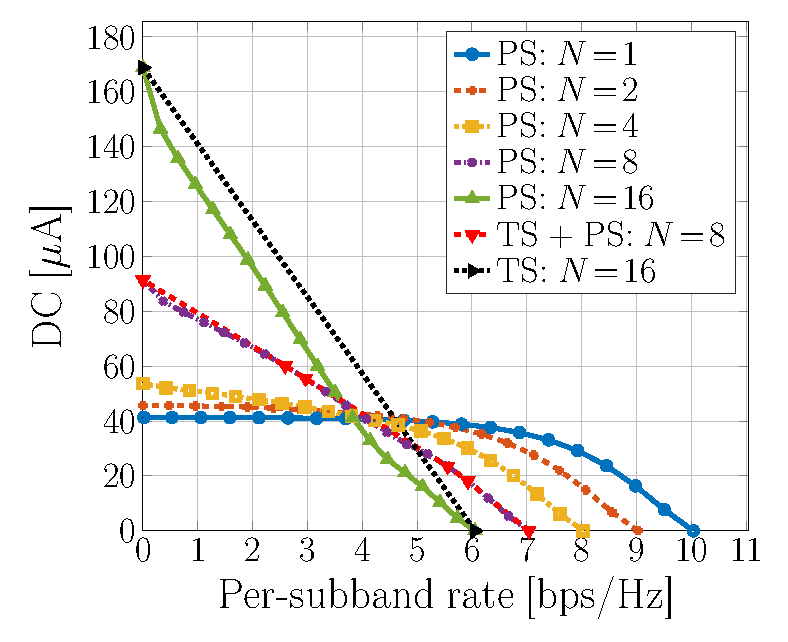
\includegraphics{assets/re_subband.eps}
				% This file was created by matlab2tikz.
%
%The latest updates can be retrieved from
%  http://www.mathworks.com/matlabcentral/fileexchange/22022-matlab2tikz-matlab2tikz
%where you can also make suggestions and rate matlab2tikz.
%
\definecolor{mycolor1}{rgb}{0.00000,0.44700,0.74100}%
\definecolor{mycolor2}{rgb}{0.85000,0.32500,0.09800}%
\definecolor{mycolor3}{rgb}{0.92900,0.69400,0.12500}%
\definecolor{mycolor4}{rgb}{0.49400,0.18400,0.55600}%
\definecolor{mycolor5}{rgb}{0.46600,0.67400,0.18800}%
%
\begin{tikzpicture}

\begin{axis}[%
width=4.036in,
height=3.396in,
at={(0.677in,0.458in)},
scale only axis,
xmin=0,
xlabel style={font=\color{white!15!black}},
xlabel={Per-subband rate [bps/Hz]},
ymin=0,
ylabel style={font=\color{white!15!black}},
ylabel={DC [$\mu$A]},
axis background/.style={fill=white},
xmajorgrids,
ymajorgrids,
legend style={legend cell align=left, align=left, draw=white!15!black},
title style={font=\huge}, label style={font=\huge}, ticklabel style={font=\LARGE}, legend style={font=\LARGE}
]
\addplot [color=mycolor1, line width=2.0pt, mark=o, mark options={solid, mycolor1}]
  table[row sep=crcr]{%
10.0371541503521	2.22044604925031e-10\\
9.50888287931245	7.67218297348236\\
8.98061160969771	16.4035328868797\\
8.45234034327624	23.7184488015709\\
7.92406907805198	29.205421549582\\
7.3957978136944	33.108418398381\\
6.86752655715228	35.8060858943009\\
6.33925531456315	37.6402604405573\\
5.81098410797576	38.8754185210755\\
5.28271290103602	39.7025741932163\\
4.75444168414669	40.2547940715469\\
4.22617042980331	40.6229044735893\\
3.69789919151785	40.8681643325841\\
3.16962794157827	41.0316006620616\\
2.64135688073796	41.1405795757475\\
2.11308593958905	41.2133145315082\\
1.58481573162	41.2619161559168\\
1.05654557443832	41.2944351162874\\
0.52831621285643	41.3162247649014\\
0.0172895850115278	41.3305512860995\\
};
\addlegendentry{PS: $N = 1$}

\addplot [color=mycolor2, dashed, line width=2.0pt, mark=+, mark options={solid, mycolor2}]
  table[row sep=crcr]{%
9.02654522797361	2.22044604925031e-10\\
8.55146390059239	6.85672511413178\\
8.07638260779107	14.9052859902322\\
7.60130144663416	22.0060908430934\\
7.12622060328784	27.6704698672712\\
6.65114024798395	32.0013219513062\\
6.17606060075074	35.260704866419\\
5.70098161136798	37.7089802785193\\
5.22590380097997	39.5578388388224\\
4.75082663535468	40.9688790179793\\
4.27575311838366	42.0598435792836\\
3.80068610434027	42.9182097430551\\
3.32564099290071	43.6116792643263\\
2.85063913633349	44.1927578797524\\
2.37567922919448	44.6914808377669\\
1.90064908156813	45.0988588665419\\
1.42547871463989	45.3685552024517\\
0.950295873559429	45.5091782183481\\
0.475137711619894	45.5794354570947\\
0.000663657492032048	45.618094965604\\
};
\addlegendentry{PS: $N = 2$}

\addplot [color=mycolor3, dotted, line width=2.0pt, mark=square, mark options={solid, mycolor3}]
  table[row sep=crcr]{%
8.02820199706102	2.22044604925031e-10\\
7.60566505005435	6.08410472686023\\
7.18312811002374	13.4005574475261\\
6.76059120575472	20.1200100568908\\
6.33805433156525	25.7129233574566\\
5.91551755675746	30.1714764925982\\
5.4929808816325	33.6681484303917\\
5.0704443009935	36.4059122716515\\
4.64790825516503	38.54188122081\\
4.22537205195086	40.2468595423231\\
3.80283703067816	41.8775306137104\\
3.38030447492251	43.508083649551\\
2.9577717028917	45.0595482422157\\
2.53524635542607	46.4648537621826\\
2.11271996143974	47.7927943480477\\
1.69019624522729	49.0171759337246\\
1.26767527574324	50.1365279807279\\
0.845142595331543	51.1646581566389\\
0.422574321530065	52.1170138397447\\
0.000277724924339261	53.7210893503867\\
};
\addlegendentry{PS: $N = 4$}

\addplot [color=mycolor4, dashdotted, line width=2.0pt, mark=x, mark options={solid, mycolor4}]
  table[row sep=crcr]{%
7.03646030601376	2.22044604925031e-10\\
6.66612029030538	5.33480531181279\\
6.29578028617171	11.8872873038635\\
5.92544032072519	18.1364536120616\\
5.55510039557916	23.546177701565\\
5.18476059643454	28.0230548332227\\
4.81442093529084	31.556742715674\\
4.44408154088595	35.8687144677689\\
4.07374243788686	40.7075485691513\\
3.7034034931988	45.7524875922775\\
3.33306615955232	50.7208251361567\\
2.96272956331252	55.5324442818824\\
2.59239482523149	60.1014296610934\\
2.22205943650744	64.4088952304281\\
1.85172505092483	68.4573630477063\\
1.48139082382635	72.2898353377071\\
1.11105543991423	75.9756365608707\\
0.740723137786698	79.6445797605057\\
0.370400218325631	83.6381061566867\\
9.45761316017172e-05	91.3623020603484\\
};
\addlegendentry{PS: $N = 8$}

\addplot [color=mycolor5, line width=2.0pt, mark=triangle, mark options={solid, mycolor5}]
  table[row sep=crcr]{%
6.05379560631091	2.22044604925031e-10\\
5.7351747874227	4.60997152282855\\
5.41655400456529	10.3758238457199\\
5.09793329283942	16.0788416628558\\
4.7793126468511	21.1796846327491\\
4.46069218004009	25.9803569336201\\
4.14207192099301	32.9144001116473\\
3.82345210911695	41.1823618505934\\
3.50483288971294	50.3051385141085\\
3.18621391242395	59.9070139410534\\
2.86759587178783	69.7183641914114\\
2.54897730209977	79.540577968307\\
2.23035844532724	89.2334238541247\\
1.91174161557065	98.7223345120381\\
1.59312669899359	107.997658714437\\
1.27451347775714	117.117862930033\\
0.955903974752901	126.238947824315\\
0.637295656505832	135.712526397667\\
0.318682366621808	146.495410665419\\
1.1818881022604e-05	168.8057828875\\
};
\addlegendentry{PS: $N = 16$}

\addplot [color=red, dashed, line width=2.0pt, mark=triangle, mark options={solid, rotate=180, red}]
  table[row sep=crcr]{%
7.03646030601376	2.22044604925031e-10\\
5.92544032072519	18.1364536120616\\
5.55510039557916	23.546177701565\\
2.96272956331252	55.5324442818824\\
2.59239482523149	60.1014296610934\\
9.45761316017172e-05	91.3623020603484\\
};
\addlegendentry{TS + PS: $N = 8$}

\addplot [color=black, dotted, line width=2.0pt, mark=triangle, mark options={solid, rotate=270, black}]
  table[row sep=crcr]{%
1.1818881022604e-05	168.8057828875\\
6.05379560631091	2.22044604925031e-10\\
};
\addlegendentry{TS: $N = 16$}

\end{axis}
\end{tikzpicture}%

			}
		}
		\subfloat[\gls{wpt} waveform amplitude\label{fi:waveform_subband}]{
			\resizebox{0.45\columnwidth}{!}{
				% 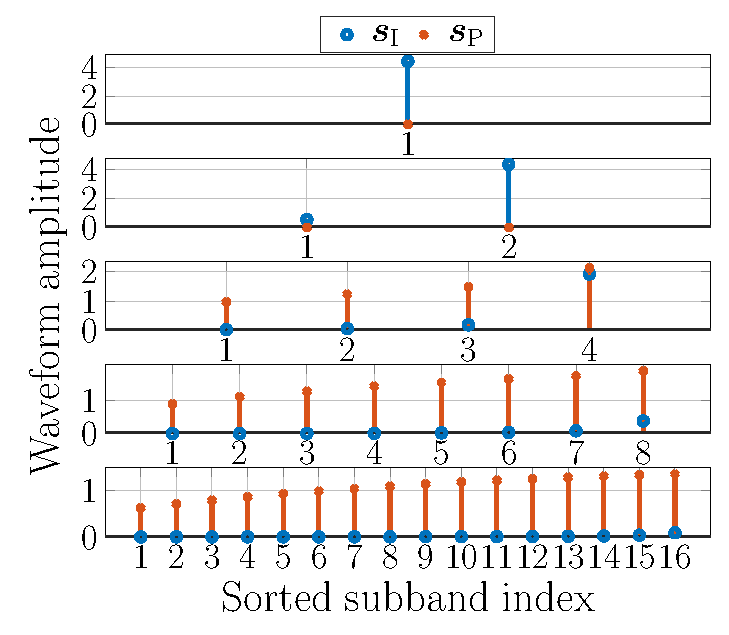
\includegraphics{assets/waveform_subband.eps}
				% This file was created by matlab2tikz.
%
%The latest updates can be retrieved from
%  http://www.mathworks.com/matlabcentral/fileexchange/22022-matlab2tikz-matlab2tikz
%where you can also make suggestions and rate matlab2tikz.
%
\definecolor{mycolor1}{rgb}{0.00000,0.44700,0.74100}%
\definecolor{mycolor2}{rgb}{0.85000,0.32500,0.09800}%
%
\begin{tikzpicture}

\begin{axis}[%
width=4.036in,
height=0.462in,
at={(0.677in,3.21in)},
scale only axis,
xmin=0,
xmax=2,
xtick={1},
ymin=0,
axis background/.style={fill=white},
xmajorgrids,
ymajorgrids,
legend style={at={(0.5,1.03)}, anchor=south, legend columns=2, legend cell align=left, align=left, draw=white!15!black},
title style={font=\huge}, label style={font=\huge}, ticklabel style={font=\LARGE}, legend style={font=\LARGE}
]
\addplot[ycomb, color=mycolor1, line width=2.0pt, mark=o, mark options={solid, mycolor1}] table[row sep=crcr] {%
1	4.47213593809508\\
};
\addplot[forget plot, color=white!15!black, line width=2.0pt] table[row sep=crcr] {%
0	0\\
2	0\\
};
\addlegendentry{{\boldmath${s}$}$_{\mathrm{I}}$}

\addplot[ycomb, color=mycolor2, line width=2.0pt, mark=x, mark options={solid, mycolor2}] table[row sep=crcr] {%
1	0.000358590327058133\\
};
\addplot[forget plot, color=white!15!black, line width=2.0pt] table[row sep=crcr] {%
0	0\\
2	0\\
};
\addlegendentry{{\boldmath${s}$}$_{\mathrm{P}}$}

\end{axis}

\begin{axis}[%
width=4.036in,
height=0.462in,
at={(0.677in,2.522in)},
scale only axis,
xmin=0,
xmax=3,
xtick={1, 2},
ymin=0,
axis background/.style={fill=white},
xmajorgrids,
ymajorgrids,
title style={font=\huge}, label style={font=\huge}, ticklabel style={font=\LARGE}, legend style={font=\LARGE}
]
\addplot[ycomb, color=mycolor1, line width=2.0pt, mark=o, mark options={solid, mycolor1}, forget plot] table[row sep=crcr] {%
1	0.550823184768846\\
2	4.36837845097092\\
};
\addplot[forget plot, color=white!15!black, line width=2.0pt] table[row sep=crcr] {%
0	0\\
3	0\\
};
\addplot[ycomb, color=mycolor2, line width=2.0pt, mark=x, mark options={solid, mycolor2}, forget plot] table[row sep=crcr] {%
1	1.48597207854411e-05\\
2	1.53805823004565e-05\\
};
\addplot[forget plot, color=white!15!black, line width=2.0pt] table[row sep=crcr] {%
0	0\\
3	0\\
};
\end{axis}

\begin{axis}[%
width=4.036in,
height=0.462in,
at={(0.677in,1.834in)},
scale only axis,
xmin=0,
xmax=5,
xtick={1, 2, 3, 4},
ymin=0,
ylabel style={font=\color{white!15!black}},
ylabel={Waveform amplitude},
axis background/.style={fill=white},
xmajorgrids,
ymajorgrids,
title style={font=\huge}, label style={font=\huge}, ticklabel style={font=\LARGE}, legend style={font=\LARGE}
]
\addplot[ycomb, color=mycolor1, line width=2.0pt, mark=o, mark options={solid, mycolor1}, forget plot] table[row sep=crcr] {%
1	0.0326721056203988\\
2	0.0697944085211443\\
3	0.193520763120912\\
4	1.91750698481035\\
};
\addplot[forget plot, color=white!15!black, line width=2.0pt] table[row sep=crcr] {%
0	0\\
5	0\\
};
\addplot[ycomb, color=mycolor2, line width=2.0pt, mark=x, mark options={solid, mycolor2}, forget plot] table[row sep=crcr] {%
1	0.972503011468572\\
2	1.22779327868874\\
3	1.48063097057209\\
4	2.13162879975205\\
};
\addplot[forget plot, color=white!15!black, line width=2.0pt] table[row sep=crcr] {%
0	0\\
5	0\\
};
\end{axis}

\begin{axis}[%
width=4.036in,
height=0.462in,
at={(0.677in,1.146in)},
scale only axis,
xmin=0,
xmax=9,
xtick={1, 2, 3, 4, 5, 6, 7, 8},
ymin=0,
ytick={0, 1},
axis background/.style={fill=white},
xmajorgrids,
ymajorgrids,
title style={font=\huge}, label style={font=\huge}, ticklabel style={font=\LARGE}, legend style={font=\LARGE}
]
\addplot[ycomb, color=mycolor1, line width=2.0pt, mark=o, mark options={solid, mycolor1}, forget plot] table[row sep=crcr] {%
1	0.00676327571402152\\
2	0.00930781551713654\\
3	0.0129863266085796\\
4	0.0182780278377859\\
5	0.0264785684252956\\
6	0.0417816477229242\\
7	0.0921547943904462\\
8	0.387871897134795\\
};
\addplot[forget plot, color=white!15!black, line width=2.0pt] table[row sep=crcr] {%
0	0\\
9	0\\
};
\addplot[ycomb, color=mycolor2, line width=2.0pt, mark=x, mark options={solid, mycolor2}, forget plot] table[row sep=crcr] {%
1	0.897080828535262\\
2	1.11267484124012\\
3	1.2760937466216\\
4	1.42973823824102\\
5	1.54367522426452\\
6	1.64897920494507\\
7	1.73956386270218\\
8	1.89059947472085\\
};
\addplot[forget plot, color=white!15!black, line width=2.0pt] table[row sep=crcr] {%
0	0\\
9	0\\
};
\end{axis}

\begin{axis}[%
width=4.036in,
height=0.462in,
at={(0.677in,0.458in)},
scale only axis,
xmin=0,
xmax=17,
xtick={ 1,  2,  3,  4,  5,  6,  7,  8,  9, 10, 11, 12, 13, 14, 15, 16},
xlabel style={font=\color{white!15!black}},
xlabel={Sorted subband index},
ymin=0,
ytick={0, 1},
axis background/.style={fill=white},
xmajorgrids,
ymajorgrids,
title style={font=\huge}, label style={font=\huge}, ticklabel style={font=\LARGE}, legend style={font=\LARGE}
]
\addplot[ycomb, color=mycolor1, line width=2.0pt, mark=o, mark options={solid, mycolor1}, forget plot] table[row sep=crcr] {%
1	0.00205132551819701\\
2	0.00235447373497551\\
3	0.00272196136127332\\
4	0.00316588966668174\\
5	0.00369517036368117\\
6	0.00432537450541609\\
7	0.00508695652011363\\
8	0.00600094215308655\\
9	0.00710012267822671\\
10	0.00851262778314969\\
11	0.0103510448032954\\
12	0.0128569172775466\\
13	0.0164283761517276\\
14	0.0229541038226562\\
15	0.0402894292810385\\
16	0.0926842285796484\\
};
\addplot[forget plot, color=white!15!black, line width=2.0pt] table[row sep=crcr] {%
0	0\\
17	0\\
};
\addplot[ycomb, color=mycolor2, line width=2.0pt, mark=x, mark options={solid, mycolor2}, forget plot] table[row sep=crcr] {%
1	0.628841069483884\\
2	0.717675502523908\\
3	0.795496148359302\\
4	0.864626670343281\\
5	0.930591126638763\\
6	0.989724762400551\\
7	1.04508455096183\\
8	1.09678731061405\\
9	1.14380160245268\\
10	1.18636001210616\\
11	1.2248217690153\\
12	1.2585853066132\\
13	1.28750705323146\\
14	1.31224542931104\\
15	1.33460858167442\\
16	1.35822969320702\\
};
\addplot[forget plot, color=white!15!black, line width=2.0pt] table[row sep=crcr] {%
0	0\\
17	0\\
};
\end{axis}
\end{tikzpicture}%
			}
		}
		\caption{Average \gls{r-e} region and \gls{wpt} waveform amplitude versus $N$ for $M=1$, $L=20$, $\sigma_n^2=\qty{-40}{dBm}$, $B=\qty{1}{\MHz}$ and $d_{\mathrm{H}}=d_{\mathrm{V}}=\qty{2}{\meter}$.}
	\end{figure}

	Fig.~\subref*{fi:re_subband} illustrates the average \gls{r-e} region versus the number of subband $N$. First, it is observed that increasing $N$ reduces the per-subband rate but boosts the harvested energy. This is because less power is allocated to each subband but more balanced \gls{dc} terms are introduced by frequency coupling to boost the harvested energy. On the other hand, Fig.~\subref*{fi:waveform_subband} presents the sorted modulated/multisine amplitude $\boldsymbol{s}_{\mathrm{I/P}}$ for \gls{wpt}. It demonstrates that a dedicated multisine waveform is unnecessary for a small $N$ but is required for a large $N$. This observation origins from the rectifier nonlinearity. Although both waveforms have equivalent second-order \gls{dc} terms \eqref{eq:y_I2} and \eqref{eq:y_P2}, for the fourth-order terms \eqref{eq:y_I4} and \eqref{eq:y_P4}, the modulated waveform has $N^2$ monomials with a modulation gain of \num{2}, while the multisine has $(2N^3+N)/3$ monomials as the components of different frequencies compensate and produce \gls{dc}. Second, the \gls{r-e} region is convex for $N \in \{2,4\}$ and concave-convex for $N \in \{8,16\}$, such that \gls{ps} outperforms \gls{ts} for a small $N$ and is outperformed for a large $N$. When $N$ is in between, the optimal strategy is a combination of both, i.e., a time sharing between the \gls{wpt} point and the saddle \gls{ps} \gls{swipt} point (as denoted by the red curve in Fig.~\subref*{fi:re_subband}). When $N$ is relatively small, only modulated waveform is used at both \gls{wit} and \gls{wpt} points, and one can infer that no multisine waveform is needed for the entire \gls{r-e} region. It aligns with the conclusion based on the conventional linear harvester model, namely the \gls{r-e} region is convex, \gls{ps} outperforms \gls{ts}, and dedicated power waveform is unnecessary. As $N$ becomes sufficiently large, the multisine waveform further boosts \gls{wpt} and creates some concavity in the high-power region, which accounts for the superiority of \gls{ts} under the nonlinear harvester model. Therefore, we conclude that the rectifier nonlinearity enlarges the \gls{r-e} region by favoring a different waveform and receiving mode, both heavily depending on $N$.

	\begin{figure}[!t]
		\centering
		\subfloat[\gls{r-e} region\label{fi:re_noise}]{
			\resizebox{0.45\columnwidth}{!}{
				% 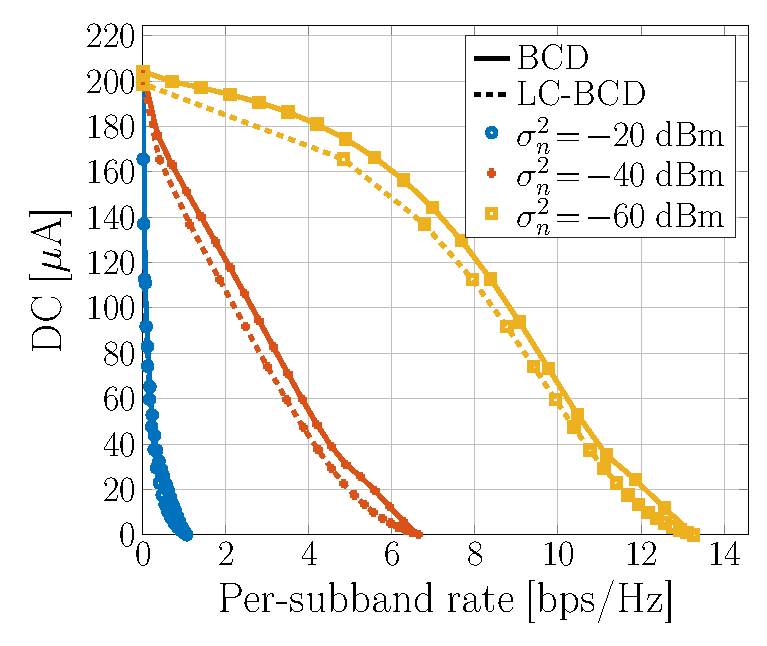
\includegraphics{assets/re_noise.eps}
				% This file was created by matlab2tikz.
%
%The latest updates can be retrieved from
%  http://www.mathworks.com/matlabcentral/fileexchange/22022-matlab2tikz-matlab2tikz
%where you can also make suggestions and rate matlab2tikz.
%
\definecolor{mycolor1}{rgb}{0.00000,0.44706,0.74118}%
\definecolor{mycolor2}{rgb}{0.85098,0.32549,0.09804}%
\definecolor{mycolor3}{rgb}{0.92941,0.69412,0.12549}%
%
\begin{tikzpicture}

\begin{axis}[%
width=4.036in,
height=3.396in,
at={(0.677in,0.458in)},
scale only axis,
xmin=0,
xlabel style={font=\color{white!15!black}},
xlabel={Per-subband rate [bps/Hz]},
ymin=0,
ylabel style={font=\color{white!15!black}},
ylabel={DC [$\mu$A]},
axis background/.style={fill=white},
xmajorgrids,
ymajorgrids,
legend style={legend cell align=left, align=left, draw=white!15!black},
title style={font=\huge}, label style={font=\huge}, ticklabel style={font=\LARGE}, legend style={font=\LARGE}
]
\addplot [color=mycolor1, line width=2.0pt, mark=o, mark options={solid, mycolor1}, forget plot]
  table[row sep=crcr]{%
1.05231544893842	2.22044604925031e-10\\
0.996936592022447	1.52924438127048\\
0.941547738715287	3.39650359894689\\
0.886160927371223	5.5654135038664\\
0.830776052795363	7.98207432016343\\
0.775392699958405	10.6017107955025\\
0.720010487964039	13.3878582888891\\
0.664628256360362	16.3123044599313\\
0.60924537524882	19.3542317254838\\
0.553861928462	22.4998186427932\\
0.49847774797173	25.7422469055075\\
0.443092369241085	28.8337551576151\\
0.387706273929563	32.4096169692436\\
0.332319831521671	37.2603838371814\\
0.276934107656023	43.7723771545919\\
0.221549270686116	52.7534525591782\\
0.166163251023552	65.245587158838\\
0.110776409955529	82.9489673694593\\
0.0553889743825141	110.935935789809\\
4.00294695505045e-10	204.115191529349\\
};
\addplot [color=mycolor1, dashed, line width=2.0pt, mark=o, mark options={solid, mycolor1}, forget plot]
  table[row sep=crcr]{%
1.05231539685191	2.22044604925031e-10\\
0.977327808474395	0.947706963284163\\
0.902257555584857	2.10296179377206\\
0.827208711201837	3.50675073105097\\
0.752420765207274	5.227298591977\\
0.678181267771261	7.36005445178743\\
0.6048303892807	10.0277017205721\\
0.532767789269605	13.3801600644627\\
0.462458593452248	17.5945764435843\\
0.394438818982741	22.8753354231855\\
0.329319098859593	29.454052299871\\
0.267785151110453	37.5895775261628\\
0.210593116270609	47.5679903073645\\
0.15855784740875	59.7025983888838\\
0.112531617630159	74.3339403496809\\
0.0733715088778041	91.8297822092195\\
0.0418950713994759	112.58511866794\\
0.0188264277980689	137.022172153013\\
0.00473845957496308	165.590394553955\\
0	198.766465264793\\
};
\addplot [color=mycolor2, line width=2.0pt, mark=+, mark options={solid, mycolor2}, forget plot]
  table[row sep=crcr]{%
6.63489989133022	2.22044604925031e-10\\
6.28569463377105	5.6382231905721\\
5.93648937653002	12.6018805448586\\
5.58728412018769	19.4788436898403\\
5.23807886717802	25.669470029177\\
4.8888736195627	31.0886536828396\\
4.539668392543	38.9426300113197\\
4.19046322167092	48.672016668236\\
3.84125805353658	59.5333310547779\\
3.49205289805752	71.0113521358651\\
3.14284763669287	82.7817515534032\\
2.7936422884944	94.6022229448075\\
2.44443693920068	106.311584054828\\
2.09523165122091	117.819806713077\\
1.74602640018096	129.109446889105\\
1.39682112159978	140.247786948107\\
1.04761629776652	151.423153846714\\
0.698416179079124	163.066082066625\\
0.349230888188612	176.366894851491\\
8.38935903068317e-08	204.11429064019\\
};
\addplot [color=mycolor2, dashed, line width=2.0pt, mark=+, mark options={solid, mycolor2}, forget plot]
  table[row sep=crcr]{%
6.63489989132575	2.22044604925031e-10\\
6.48083859286744	0.935538588478854\\
6.31826373705624	2.07674485193581\\
6.14613309127056	3.46518046769842\\
5.9632758302973	5.1696442739292\\
5.76829950217088	7.28616429982432\\
5.55952562082815	9.93800219032707\\
5.33491102921871	13.2756440618395\\
5.09194173223281	17.4768064353061\\
4.82748309819336	22.7464394980837\\
4.53756886232237	29.3167154766308\\
4.21710987607214	37.447041334489\\
3.85948370708577	47.4240540895343\\
3.45597658817774	59.56162225694\\
2.9951173958276	74.2008462847387\\
2.46227201500798	91.7100547106112\\
1.84137965867656	112.48481197181\\
1.12765427290716	136.947911008074\\
0.391777715662229	165.549377437517\\
0	198.766465224913\\
};
\addplot [color=mycolor3, line width=2.0pt, mark=square, mark options={solid, mycolor3}, forget plot]
  table[row sep=crcr]{%
13.261275561803	2.22044604925031e-10\\
12.5633136900684	11.8097368751011\\
11.8653518185617	24.2808808858222\\
11.1673899473727	35.1529677129197\\
10.4694280776483	52.9746784546842\\
9.77146620548022	73.3395988435084\\
9.07350433337152	93.7483281565825\\
8.37554246161132	112.776924198566\\
7.67758059210468	129.674867620128\\
6.97961872226381	144.175676082331\\
6.28165685341863	156.319500851227\\
5.58369498790593	166.314925805355\\
4.88573312504996	174.445410226985\\
4.18777128855024	181.012371001491\\
3.48980951755386	186.304713485142\\
2.791847984205	190.586818111533\\
2.09388727434806	194.098527562363\\
1.39592886128892	197.069415619306\\
0.69796609362423	199.78743280114\\
7.19406549031101e-06	204.114232297971\\
};
\addplot [color=mycolor3, dashed, line width=2.0pt, mark=square, mark options={solid, mycolor3}, forget plot]
  table[row sep=crcr]{%
13.26127555768	2.22044604925031e-10\\
13.1052417587908	0.935422212373737\\
12.940333826529	2.07649106322328\\
12.7654265103412	3.46477607266082\\
12.5792313693343	5.16908124112507\\
12.3801910384352	7.28544176208695\\
12.1664022666181	9.9371218039785\\
11.9355039976223	13.2746167153488\\
11.6845184111854	17.4756478372\\
11.4096155861423	22.7451666809748\\
11.1057545104633	29.3153561572846\\
10.7661102340862	37.4456281078633\\
10.3811242700452	47.4226241423339\\
9.93681047823449	59.560220427702\\
9.41152464991377	74.1995191235079\\
8.7691099146231	91.7088599928581\\
7.94214427637187	112.48380827719\\
6.7810510476787	136.947164162744\\
4.82745854264995	165.548963540215\\
0	198.766466242674\\
};
\addplot [color=black, line width=2.0pt]
  table[row sep=crcr]{%
-1	-1\\
};
\addlegendentry{BCD}

\addplot [color=black, dashed, line width=2.0pt]
  table[row sep=crcr]{%
-1	-1\\
};
\addlegendentry{LC-BCD}

\addplot [color=mycolor1, line width=2.0pt, only marks, mark=o, mark options={solid, mycolor1}]
  table[row sep=crcr]{%
-1	-1\\
};
\addlegendentry{$\sigma_n^2 = -20$ dBm}

\addplot [color=mycolor2, line width=2.0pt, only marks, mark=+, mark options={solid, mycolor2}]
  table[row sep=crcr]{%
-1	-1\\
};
\addlegendentry{$\sigma_n^2 = -40$ dBm}

\addplot [color=mycolor3, line width=2.0pt, only marks, mark=square, mark options={solid, mycolor3}]
  table[row sep=crcr]{%
-1	-1\\
};
\addlegendentry{$\sigma_n^2 = -60$ dBm}

\end{axis}
\end{tikzpicture}%
			}
		}
		\subfloat[Splitting ratio\label{fi:splitting_ratio_noise}]{
			\resizebox{0.45\columnwidth}{!}{
				% 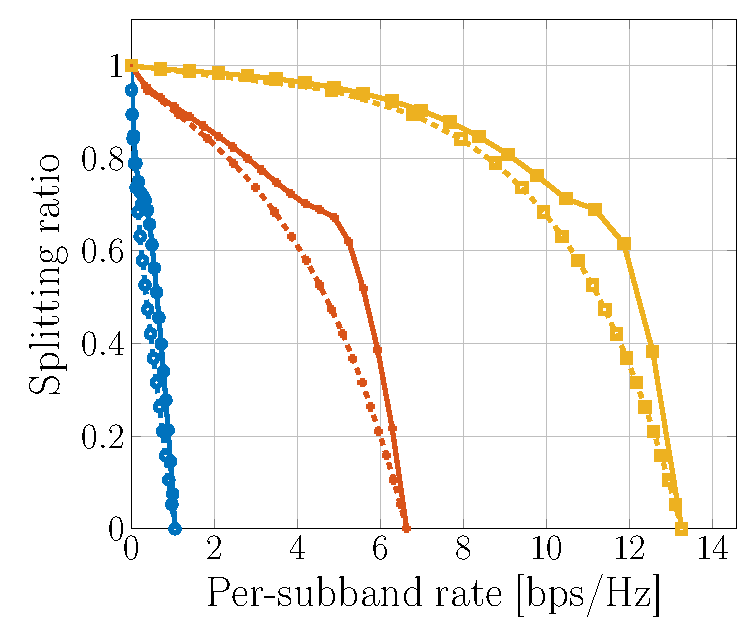
\includegraphics{assets/splitting_ratio_noise.eps}
				% This file was created by matlab2tikz.
%
%The latest updates can be retrieved from
%  http://www.mathworks.com/matlabcentral/fileexchange/22022-matlab2tikz-matlab2tikz
%where you can also make suggestions and rate matlab2tikz.
%
\definecolor{mycolor1}{rgb}{0.00000,0.44706,0.74118}%
\definecolor{mycolor2}{rgb}{0.85098,0.32549,0.09804}%
\definecolor{mycolor3}{rgb}{0.92941,0.69412,0.12549}%
%
\begin{tikzpicture}

\begin{axis}[%
width=4.036in,
height=3.396in,
at={(0.677in,0.458in)},
scale only axis,
xmin=0,
xlabel style={font=\color{white!15!black}},
xlabel={Per-subband rate [bps/Hz]},
ymin=0,
ylabel style={font=\color{white!15!black}},
ylabel={Splitting ratio},
axis background/.style={fill=white},
xmajorgrids,
ymajorgrids,
title style={font=\huge}, label style={font=\huge}, ticklabel style={font=\LARGE}, legend style={font=\LARGE}
]
\addplot [color=mycolor1, line width=2.0pt, mark=o, mark options={solid, mycolor1}, forget plot]
  table[row sep=crcr]{%
1.05231544893842	2.22044604925031e-16\\
0.996936592022447	0.0754506573452514\\
0.941547738715287	0.145592699046563\\
0.886160927371223	0.212907606612686\\
0.830776052795363	0.277500373362808\\
0.775392699958405	0.33947082813972\\
0.720010487964039	0.398923222548953\\
0.664628256360362	0.455934802355196\\
0.60924537524882	0.510599550575608\\
0.553861928462	0.563051709054834\\
0.49847774797173	0.613442753059218\\
0.443092369241085	0.657526311613642\\
0.387706273929563	0.688283323153185\\
0.332319831521671	0.709092322018303\\
0.276934107656023	0.719406940830095\\
0.221549270686116	0.72581496878029\\
0.166163251023552	0.749089663981749\\
0.110776409955529	0.789063650376257\\
0.0553889743825141	0.848328541972237\\
4.00294695505045e-10	0.999989573696362\\
};
\addplot [color=mycolor1, dashed, line width=2.0pt, mark=o, mark options={solid, mycolor1}, forget plot]
  table[row sep=crcr]{%
1.05231539685191	2.22044604925031e-16\\
0.977327808474395	0.0526315789473685\\
0.902257555584857	0.105263157894737\\
0.827208711201837	0.157894736842105\\
0.752420765207274	0.210526315789474\\
0.678181267771261	0.263157894736842\\
0.6048303892807	0.315789473684211\\
0.532767789269605	0.368421052631579\\
0.462458593452248	0.421052631578947\\
0.394438818982741	0.473684210526315\\
0.329319098859593	0.526315789473685\\
0.267785151110453	0.578947368421053\\
0.210593116270609	0.631578947368421\\
0.15855784740875	0.68421052631579\\
0.112531617630159	0.736842105263158\\
0.0733715088778041	0.789473684210527\\
0.0418950713994759	0.842105263157894\\
0.0188264277980689	0.894736842105263\\
0.00473845957496308	0.947368421052631\\
0	1\\
};
\addplot [color=mycolor2, line width=2.0pt, mark=+, mark options={solid, mycolor2}, forget plot]
  table[row sep=crcr]{%
6.63489989133022	2.22044604925031e-16\\
6.28569463377105	0.216824181364595\\
5.93648937653002	0.386024188873107\\
5.58728412018769	0.517973961492521\\
5.23807886717802	0.620757696734013\\
4.8888736195627	0.672337322381988\\
4.539668392543	0.6892276031786\\
4.19046322167092	0.701737522260632\\
3.84125805353658	0.723357211364089\\
3.49205289805752	0.747906073690987\\
3.14284763669287	0.774553395603111\\
2.7936422884944	0.800245786546777\\
2.44443693920068	0.824658741615259\\
2.09523165122091	0.847690407130278\\
1.74602640018096	0.869509974581019\\
1.39682112159978	0.890346649326468\\
1.04761629776652	0.910697710604079\\
0.698416179079124	0.931383328750487\\
0.349230888188612	0.954400219449963\\
8.38935903068317e-08	0.999983887992293\\
};
\addplot [color=mycolor2, dashed, line width=2.0pt, mark=+, mark options={solid, mycolor2}, forget plot]
  table[row sep=crcr]{%
6.63489989132575	2.22044604925031e-16\\
6.48083859286744	0.0526315789473685\\
6.31826373705624	0.105263157894737\\
6.14613309127056	0.157894736842105\\
5.9632758302973	0.210526315789474\\
5.76829950217088	0.263157894736842\\
5.55952562082815	0.315789473684211\\
5.33491102921871	0.368421052631579\\
5.09194173223281	0.421052631578947\\
4.82748309819336	0.473684210526315\\
4.53756886232237	0.526315789473685\\
4.21710987607214	0.578947368421053\\
3.85948370708577	0.631578947368421\\
3.45597658817774	0.68421052631579\\
2.9951173958276	0.736842105263158\\
2.46227201500798	0.789473684210527\\
1.84137965867656	0.842105263157894\\
1.12765427290716	0.894736842105263\\
0.391777715662229	0.947368421052631\\
0	1\\
};
\addplot [color=mycolor3, line width=2.0pt, mark=square, mark options={solid, mycolor3}, forget plot]
  table[row sep=crcr]{%
13.261275561803	2.22044604925031e-16\\
12.5633136900684	0.382422577220022\\
11.8653518185617	0.615841206981419\\
11.1673899473727	0.689944820223012\\
10.4694280776483	0.71268810623127\\
9.77146620548022	0.762372832502591\\
9.07350433337152	0.808229651896233\\
8.37554246161132	0.846744786388545\\
7.67758059210468	0.878215005759902\\
6.97961872226381	0.903583224109571\\
6.28165685341863	0.923895535714522\\
5.58369498790593	0.94010412739178\\
4.88573312504996	0.953025517160894\\
4.18777128855024	0.963345201020776\\
3.48980951755386	0.971623259572724\\
2.791847984205	0.978325805205776\\
2.09388727434806	0.983848129442474\\
1.39592886128892	0.988561366109714\\
0.69796609362423	0.992936691804235\\
7.19406549031101e-06	0.999984451356334\\
};
\addplot [color=mycolor3, dashed, line width=2.0pt, mark=square, mark options={solid, mycolor3}, forget plot]
  table[row sep=crcr]{%
13.26127555768	2.22044604925031e-16\\
13.1052417587908	0.0526315789473685\\
12.940333826529	0.105263157894737\\
12.7654265103412	0.157894736842105\\
12.5792313693343	0.210526315789474\\
12.3801910384352	0.263157894736842\\
12.1664022666181	0.315789473684211\\
11.9355039976223	0.368421052631579\\
11.6845184111854	0.421052631578947\\
11.4096155861423	0.473684210526315\\
11.1057545104633	0.526315789473685\\
10.7661102340862	0.578947368421053\\
10.3811242700452	0.631578947368421\\
9.93681047823449	0.68421052631579\\
9.41152464991377	0.736842105263158\\
8.7691099146231	0.789473684210527\\
7.94214427637187	0.842105263157894\\
6.7810510476787	0.894736842105263\\
4.82745854264995	0.947368421052631\\
0	1\\
};
\end{axis}
\end{tikzpicture}%
			}
		}
		\caption{Average \gls{r-e} region and splitting ratio versus $\sigma_n^2$ for $M=1$, $N=16$, $L=20$, $B=\qty{1}{\MHz}$ and $d_{\mathrm{H}}=d_{\mathrm{V}}=\qty{2}{\meter}$.}
	\end{figure}

	The average noise power influences the \gls{r-e} region as shown in Fig.~\subref*{fi:re_noise}. First, we note that the \gls{r-e} region is roughly concave/convex at low/high \gls{snr} such that \gls{ts}/\gls{ps} are preferred correspondingly. At low \gls{snr}, the power is allocated to the modulated waveform on a few strongest subbands to achieve a high rate. As the rate constraint $\bar{R}$ decreases, Algorithm~\ref{al:gp} activates more subbands that further boosts the harvested \gls{dc} power because of frequency coupling and harvester nonlinearity. Second, there exists a turning point in the \gls{r-e} region, especially for a low noise level ($\sigma_n^2 \le \qty{-40}{dBm}$). The reason is that when $\bar{R}$ departs slightly from the maximum value, the algorithm tends to adjust the splitting ratio $\rho$ rather than allocate more power to the multisine waveform, since a small amplitude multisine could be inefficient for energy purpose. As $\bar{R}$ further decreases, thanks to the advantage of multisine, a superposed waveform with a small $\rho$ can outperform a modulated waveform with a large $\rho$. The result proves the benefit of superposed waveform and the necessity of joint waveform and splitting ratio optimization. Besides, the \gls{lc}-\gls{bcd} algorithm achieves a good balance between performance and complexity even if one-dimensional search is considered for $\delta=\rho$ from \num{0} to \num{1}.

	\begin{figure}[!t]
		\centering
		\subfloat[\gls{r-e} region\label{fi:re_distance}]{
			\resizebox{0.45\columnwidth}{!}{
				% 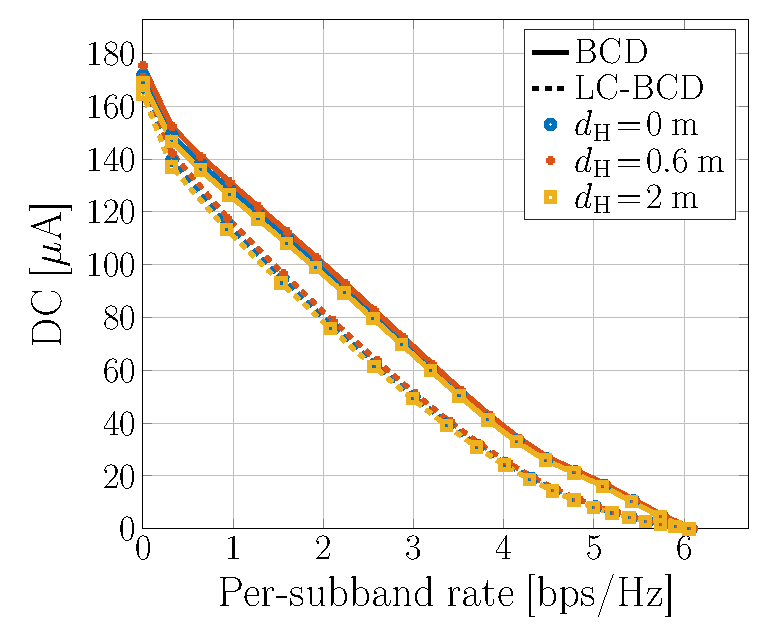
\includegraphics{assets/re_distance.eps}
				% This file was created by matlab2tikz.
%
%The latest updates can be retrieved from
%  http://www.mathworks.com/matlabcentral/fileexchange/22022-matlab2tikz-matlab2tikz
%where you can also make suggestions and rate matlab2tikz.
%
\definecolor{mycolor1}{rgb}{0.00000,0.44706,0.74118}%
\definecolor{mycolor2}{rgb}{0.85098,0.32549,0.09804}%
\definecolor{mycolor3}{rgb}{0.92941,0.69412,0.12549}%
%
\begin{tikzpicture}

\begin{axis}[%
width=4.036in,
height=3.396in,
at={(0.677in,0.458in)},
scale only axis,
xmin=0,
xlabel style={font=\color{white!15!black}},
xlabel={Per-subband rate [bps/Hz]},
ymin=0,
ylabel style={font=\color{white!15!black}},
ylabel={DC [$\mu$A]},
axis background/.style={fill=white},
xmajorgrids,
ymajorgrids,
legend style={legend cell align=left, align=left, draw=white!15!black},
title style={font=\huge}, label style={font=\huge}, ticklabel style={font=\LARGE}, legend style={font=\LARGE}
]
\addplot [color=mycolor1, line width=2.0pt, mark=o, mark options={solid, mycolor1}, forget plot]
  table[row sep=crcr]{%
6.07639216737767	2.22044604925031e-10\\
5.75658205507782	4.68346568992619\\
5.43677195804186	10.547672785567\\
5.11696190827751	16.3487495640303\\
4.79715189257578	21.5373686970265\\
4.47734204284416	26.4212494172294\\
4.15753240236261	33.4912143339499\\
3.83772333140588	41.9268945857544\\
3.5179147645604	51.226276693492\\
3.19810623145227	61.0101905383388\\
2.87829860189549	71.0078321653743\\
2.55849146435657	81.0128289984325\\
2.23868300432351	90.885220841001\\
1.91887706378631	100.546946241729\\
1.59907232543377	109.988867452961\\
1.27926956212065	119.271551670844\\
0.95947066235198	128.552389857364\\
0.639672333929743	138.189553202075\\
0.31987068030735	149.156430696188\\
9.04249861382734e-06	171.840530948475\\
};
\addplot [color=mycolor1, dashed, line width=2.0pt, mark=o, mark options={solid, mycolor1}, forget plot]
  table[row sep=crcr]{%
6.07639216734193	2.22044604925031e-10\\
5.92355314011523	0.767950441020661\\
5.76311111486512	1.70985694932238\\
5.59349915383265	2.86087818922574\\
5.41364103197	4.27912459022185\\
5.22226743431678	6.04565264794096\\
5.0178696725879	8.26445967329311\\
4.79863502691447	11.0624846931119\\
4.56235572656297	14.5896066557398\\
4.30632457165071	19.0186480994589\\
4.0271851919915	24.5453693149142\\
3.72073387826893	31.3884756696881\\
3.38166901393585	39.7896143593261\\
3.00328707938401	50.013377474753\\
2.57724217806526	62.3472994078568\\
2.09377539407344	77.1018596006774\\
1.54407806640528	94.610483804077\\
0.931499776450577	115.229541690501\\
0.320237759186487	139.338347083948\\
0	167.339158818648\\
};
\addplot [color=mycolor2, line width=2.0pt, mark=+, mark options={solid, mycolor2}, forget plot]
  table[row sep=crcr]{%
6.10306525417565	2.22044604925031e-10\\
5.78185129494814	4.766554653376\\
5.46063734721686	10.7440324263029\\
5.13942344761419	16.6583981104867\\
4.81820957743206	21.9480824714151\\
4.49699585957799	26.9416085213851\\
4.17578235380879	34.1738103905144\\
3.85456916936148	42.7993311746171\\
3.53335646618607	52.3072412100556\\
3.21214425050835	62.3065854904628\\
2.89093196098997	72.5217896604367\\
2.56972082949312	82.7394019977669\\
2.24850952835996	92.8180342576551\\
1.92729955385826	102.677741022335\\
1.6060912072511	112.310688577775\\
1.28488355604678	121.777752380964\\
0.963680592813712	131.239790146441\\
0.642478931609866	141.059336219623\\
0.321273154665288	152.232356531435\\
6.29987722710198e-06	175.330285005381\\
};
\addplot [color=mycolor2, dashed, line width=2.0pt, mark=+, mark options={solid, mycolor2}, forget plot]
  table[row sep=crcr]{%
6.10306525410346	2.22044604925031e-10\\
5.95013053214401	0.778628272680337\\
5.78956347435658	1.73482000081696\\
5.6197999939161	2.90446717870935\\
5.43976442976366	4.34689590877564\\
5.24818137362407	6.14485957385668\\
5.04353261648831	8.40453533569704\\
4.82399557425605	11.255522491121\\
4.58734812613244	14.8508428808178\\
4.33086320928084	19.36694183997\\
4.05115823750414	25.0036864106464\\
3.74399199741475	31.9843694739669\\
3.4040047025539	40.5557081633551\\
3.02441136210165	50.9878416436037\\
2.59673716616108	63.574341543647\\
2.1110246889595	78.6322013250674\\
1.55816076644374	96.5018413458497\\
0.941101839568407	117.54711015074\\
0.32404568183864	142.155282299884\\
0	170.73705939321\\
};
\addplot [color=mycolor3, line width=2.0pt, mark=square, mark options={solid, mycolor3}, forget plot]
  table[row sep=crcr]{%
6.05421017995697	2.22044604925031e-10\\
5.7355675409021	4.61596438109846\\
5.41692491950558	10.3883026922439\\
5.09828234610778	16.0975578401805\\
4.77963981954885	21.204031839939\\
4.46099745718216	26.00804369737\\
4.1423553969698	32.9418344000304\\
3.82371382363673	41.2174495773068\\
3.50507279936237	50.3490006551622\\
3.18643207757209	59.9605889400761\\
2.86779226277586	69.7824867032565\\
2.54915189798937	79.6157848833847\\
2.23051126748465	89.3202159113171\\
1.91187274100566	98.8210427633298\\
1.59323605455083	108.10855389047\\
1.27460101960929	117.241397554009\\
0.95596967986641	126.375562925547\\
0.637339209325662	135.86334891575\\
0.31870384785446	146.664055204463\\
1.17818968526279e-05	169.011957424579\\
};
\addplot [color=mycolor3, dashed, line width=2.0pt, mark=square, mark options={solid, mycolor3}, forget plot]
  table[row sep=crcr]{%
6.05421017980692	2.22044604925031e-10\\
5.90146032023079	0.759235261749169\\
5.74112375147496	1.6895038985576\\
5.57164098793648	2.82536974830512\\
5.39193420291441	4.22395957959244\\
5.20073922211266	5.96495404364483\\
4.9965572086309	8.15058508727367\\
4.77758143097754	10.9056355325392\\
4.54161747978374	14.377440012999\\
4.28597234388254	18.7358822610808\\
4.00731353782852	24.1733999857699\\
3.70146888165083	30.9049800429594\\
3.36318192543706	39.1681625229982\\
2.98581909367592	49.2230419140113\\
2.56113956314928	61.3522668886417\\
2.07954773255165	75.8610385255635\\
1.53248312072039	93.0771137008547\\
0.92361225393993	113.35080268916\\
0.317118866143085	137.05497235238\\
0	164.585043335236\\
};
\addplot [color=black, line width=2.0pt]
  table[row sep=crcr]{%
-1	-1\\
};
\addlegendentry{BCD}

\addplot [color=black, dashed, line width=2.0pt]
  table[row sep=crcr]{%
-1	-1\\
};
\addlegendentry{LC-BCD}

\addplot [color=mycolor1, line width=2.0pt, only marks, mark=o, mark options={solid, mycolor1}]
  table[row sep=crcr]{%
-1	-1\\
};
\addlegendentry{$d_{\mathrm{H}} = 0$ m}

\addplot [color=mycolor2, line width=2.0pt, only marks, mark=+, mark options={solid, mycolor2}]
  table[row sep=crcr]{%
-1	-1\\
};
\addlegendentry{$d_{\mathrm{H}} = 0.6$ m}

\addplot [color=mycolor3, line width=2.0pt, only marks, mark=square, mark options={solid, mycolor3}]
  table[row sep=crcr]{%
-1	-1\\
};
\addlegendentry{$d_{\mathrm{H}} = 2$ m}

\end{axis}
\end{tikzpicture}%

			}
		}
		\subfloat[Path loss product\label{fi:path_loss}]{
			\resizebox{0.45\columnwidth}{!}{
				% 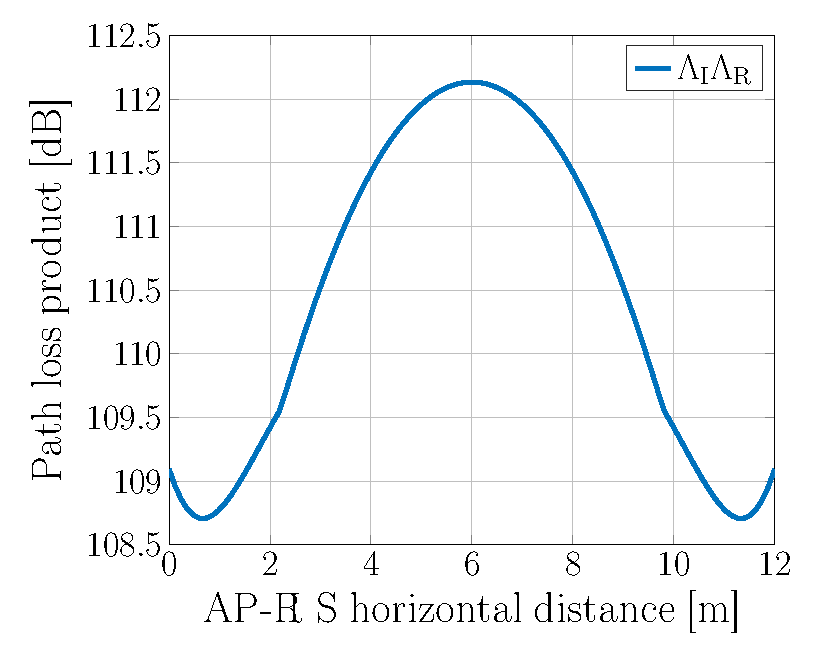
\includegraphics{assets/path_loss.eps}
				% This file was created by matlab2tikz.
%
%The latest updates can be retrieved from
%  http://www.mathworks.com/matlabcentral/fileexchange/22022-matlab2tikz-matlab2tikz
%where you can also make suggestions and rate matlab2tikz.
%
\definecolor{mycolor1}{rgb}{0.00000,0.44700,0.74100}%
%
\begin{tikzpicture}

\begin{axis}[%
width=4.036in,
height=3.396in,
at={(0.677in,0.458in)},
scale only axis,
xmin=0,
xmax=12,
xlabel style={font=\color{white!15!black}},
xlabel={AP-RIS horizontal distance [m]},
ymin=108.5,
ymax=112.5,
ylabel style={font=\color{white!15!black}},
ylabel={Path loss product [dB]},
axis background/.style={fill=white},
xmajorgrids,
ymajorgrids,
legend style={legend cell align=left, align=left, draw=white!15!black},
title style={font=\huge}, label style={font=\huge}, ticklabel style={font=\LARGE}, legend style={font=\LARGE}
]
\addplot [color=mycolor1, line width=2.0pt]
  table[row sep=crcr]{%
0	109.092173973253\\
0.121212121212121	108.957989885611\\
0.242424242424242	108.853849851555\\
0.363636363636364	108.778709266219\\
0.484848484848485	108.730923940143\\
0.606060606060606	108.708356996393\\
0.727272727272727	108.708507643881\\
0.848484848484849	108.728646669642\\
0.96969696969697	108.765945206445\\
1.09090909090909	108.817586867847\\
1.21212121212121	108.880857551026\\
1.33333333333333	108.953211109462\\
1.45454545454545	109.032312095004\\
1.57575757575758	109.116058661837\\
1.6969696969697	109.202589606194\\
1.81818181818182	109.290279630115\\
1.93939393939394	109.377726544568\\
2.06060606060606	109.463733508938\\
2.18181818181818	109.547288716316\\
2.3030303030303	109.692311186685\\
2.42424242424242	109.847121688993\\
2.54545454545455	109.998263604524\\
2.66666666666667	110.145282375612\\
2.78787878787879	110.28781386493\\
2.90909090909091	110.425570172316\\
3.03030303030303	110.55832724852\\
3.15151515151515	110.685914181524\\
3.27272727272727	110.808203999984\\
3.39393939393939	110.925105827072\\
3.51515151515152	111.036558219401\\
3.63636363636364	111.142523534753\\
3.75757575757576	111.242983185466\\
3.87878787878788	111.337933649226\\
4	111.427383124264\\
4.12121212121212	111.511348730528\\
4.24242424242424	111.589854171962\\
4.36363636363636	111.66292778719\\
4.48484848484848	111.73060092674\\
4.60606060606061	111.792906604338\\
4.72727272727273	111.849878378029\\
4.84848484848485	111.901549423862\\
4.96969696969697	111.947951770932\\
5.09090909090909	111.989115671669\\
5.21212121212121	112.025069085651\\
5.33333333333333	112.055837258945\\
5.45454545454545	112.081442384136\\
5.57575757575758	112.101903328956\\
5.6969696969697	112.117235423766\\
5.81818181818182	112.127450300185\\
5.93939393939394	112.132555774984\\
6.06060606060606	112.132555774984\\
6.18181818181818	112.127450300185\\
6.3030303030303	112.117235423766\\
6.42424242424242	112.101903328956\\
6.54545454545455	112.081442384136\\
6.66666666666667	112.055837258945\\
6.78787878787879	112.025069085651\\
6.90909090909091	111.989115671669\\
7.03030303030303	111.947951770932\\
7.15151515151515	111.901549423862\\
7.27272727272727	111.849878378029\\
7.39393939393939	111.792906604338\\
7.51515151515152	111.73060092674\\
7.63636363636364	111.66292778719\\
7.75757575757576	111.589854171962\\
7.87878787878788	111.511348730528\\
8	111.427383124264\\
8.12121212121212	111.337933649226\\
8.24242424242424	111.242983185466\\
8.36363636363636	111.142523534753\\
8.48484848484848	111.036558219401\\
8.60606060606061	110.925105827072\\
8.72727272727273	110.808203999984\\
8.84848484848485	110.685914181524\\
8.96969696969697	110.55832724852\\
9.09090909090909	110.425570172316\\
9.21212121212121	110.28781386493\\
9.33333333333333	110.145282375612\\
9.45454545454546	109.998263604524\\
9.57575757575758	109.847121688993\\
9.6969696969697	109.692311186685\\
9.81818181818182	109.547288716316\\
9.93939393939394	109.463733508938\\
10.0606060606061	109.377726544568\\
10.1818181818182	109.290279630115\\
10.3030303030303	109.202589606194\\
10.4242424242424	109.116058661837\\
10.5454545454545	109.032312095004\\
10.6666666666667	108.953211109462\\
10.7878787878788	108.880857551026\\
10.9090909090909	108.817586867847\\
11.030303030303	108.765945206445\\
11.1515151515152	108.728646669642\\
11.2727272727273	108.708507643881\\
11.3939393939394	108.708356996393\\
11.5151515151515	108.730923940143\\
11.6363636363636	108.778709266219\\
11.7575757575758	108.853849851555\\
11.8787878787879	108.957989885611\\
12	109.092173973253\\
};
\addlegendentry{$\Lambda_{\mathrm{I}}\Lambda_{\mathrm{R}}$}

\end{axis}
\end{tikzpicture}%

			}
		}
		\caption{Average \gls{r-e} region and path loss versus $d_{\mathrm{H}}$ for $M=1$, $N=16$, $L=20$, $\sigma_n^2=\qty{-40}{dBm}$, $B=\qty{1}{\MHz}$ and $d_{\mathrm{V}}=\qty{2}{\meter}$.}
	\end{figure}

	In Fig.~\subref*{fi:re_distance}, we compare the average \gls{r-e} region achieved by different \gls{ap}-\gls{ris} horizontal distance $d_{\mathrm{H}}$. Different from the active Amplify-and-Forward (AF) relay that favors midpoint development \cite{Li2017}, the \gls{ris} should be placed close to either the \gls{ap} or the \gls{ue} based on the product path loss model that applies to finite-size element reflection \cite{Ozdogan2020,Tang2021}. Moreover, there exist two optimal \gls{ris} coordinates around $d_{\mathrm{H}}=0.6$ and \qty{11.4}{\meter} that minimize the path loss product $\Lambda_{\mathrm{I}}\Lambda_R$ and maximize the \gls{r-e} tradeoff. It suggests that equipping the \gls{ap} with a \gls{ris} can potentially extend the operation range of \gls{swipt} systems.

	\begin{figure}[!t]
		\centering
		\subfloat[\gls{r-e} region\label{fi:re_tx}]{
			\resizebox{0.45\columnwidth}{!}{
				% 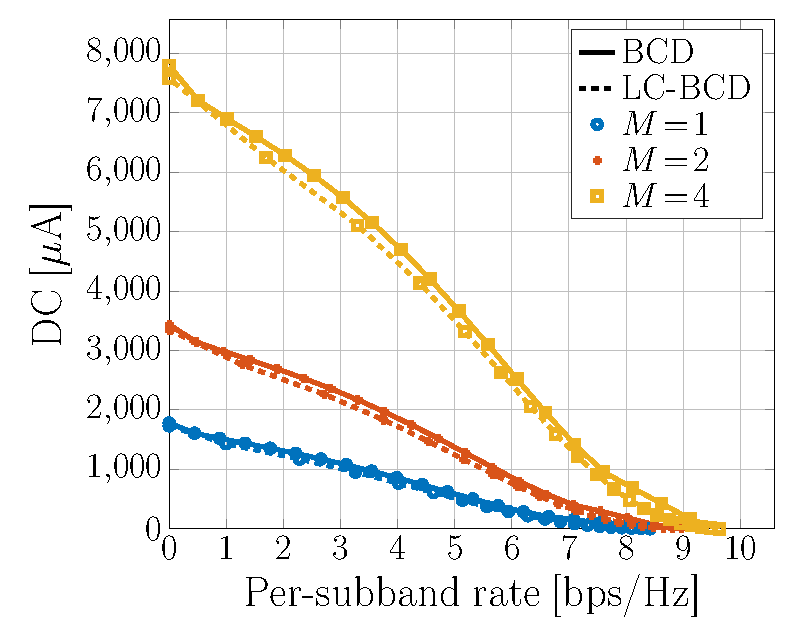
\includegraphics{assets/re_tx.eps}
				% This file was created by matlab2tikz.
%
%The latest updates can be retrieved from
%  http://www.mathworks.com/matlabcentral/fileexchange/22022-matlab2tikz-matlab2tikz
%where you can also make suggestions and rate matlab2tikz.
%
\definecolor{mycolor1}{rgb}{0.00000,0.44706,0.74118}%
\definecolor{mycolor2}{rgb}{0.85098,0.32549,0.09804}%
\definecolor{mycolor3}{rgb}{0.92941,0.69412,0.12549}%
%
\begin{tikzpicture}

\begin{axis}[%
width=4.036in,
height=3.396in,
at={(0.677in,0.458in)},
scale only axis,
xmin=0,
xlabel style={font=\color{white!15!black}},
xlabel={Per-subband rate [bps/Hz]},
ymin=0,
ylabel style={font=\color{white!15!black}},
ylabel={DC [$\mu$A]},
axis background/.style={fill=white},
xmajorgrids,
ymajorgrids,
legend style={legend cell align=left, align=left, draw=white!15!black},
title style={font=\huge}, label style={font=\huge}, ticklabel style={font=\LARGE}, legend style={font=\LARGE}
]
\addplot [color=mycolor1, line width=2.0pt, mark=o, mark options={solid, mycolor1}, forget plot]
  table[row sep=crcr]{%
8.41634063590626	2.22044604925031e-10\\
7.97337533922116	38.1656969537664\\
7.53041004261696	95.9603537470489\\
7.08744474604978	153.638185422508\\
6.6444794496291	202.982715195943\\
6.20151415485593	284.631904581804\\
5.75854885750789	388.137157143669\\
5.31558355981793	502.313124556595\\
4.87261826295901	621.547747674186\\
4.42965296638649	741.402107165695\\
3.98668766984615	858.557251217265\\
3.5437223732667	970.761793679867\\
3.10075707689241	1076.70902388285\\
2.65779178045439	1175.89537354523\\
2.21482648395747	1268.50613351711\\
1.77186118756735	1355.37831219634\\
1.32889589672681	1438.13778107542\\
0.885930870773369	1519.7793085076\\
0.442969033583207	1607.70433515463\\
1.29075269293407e-09	1779.02605419175\\
};
\addplot [color=mycolor1, dashed, line width=2.0pt, mark=o, mark options={solid, mycolor1}, forget plot]
  table[row sep=crcr]{%
8.41634063547231	2.22044604925031e-10\\
8.26072711095605	3.56591751280798\\
8.09640454350064	9.00834884036251\\
7.92220042640104	16.7082747404761\\
7.73685793901715	27.2979268152845\\
7.53886328639608	41.6607629600944\\
7.32637795921357	60.9314383167105\\
7.0971277212009	86.4957837938718\\
6.84826348316087	119.990824602809\\
6.57615090140979	163.304781247683\\
6.27605525896145	218.577047796754\\
5.94165965662905	288.19824920117\\
5.56428721254018	374.810207584034\\
5.13160417299915	481.305954016571\\
4.62534129330765	610.829754166725\\
4.01710951224429	766.777076110591\\
3.2605902541228	952.794607813459\\
2.2795714834892	1172.7802703747\\
0.994467026208467	1430.8831883225\\
0	1731.50369189428\\
};
\addplot [color=mycolor2, line width=2.0pt, mark=+, mark options={solid, mycolor2}, forget plot]
  table[row sep=crcr]{%
8.96761694708257	2.22044604925031e-10\\
8.49563710768334	71.9119527153475\\
8.02365726840095	185.276920470732\\
7.5516774291353	297.537574957316\\
7.07969758995629	399.941223933671\\
6.60771775092227	581.017651072344\\
6.13573791145558	797.265445153023\\
5.66375807188205	1032.27847035099\\
5.19177823260432	1274.4161753819\\
4.7197983933711	1514.54867784857\\
4.24781855409761	1746.10279726562\\
3.77583871486715	1964.85669098393\\
3.30385887584874	2168.57975502984\\
2.83187903662771	2356.66189042518\\
2.35989919734468	2529.80693937088\\
1.88791935815044	2689.89174219068\\
1.41593951916303	2840.144641654\\
0.943959735662882	2986.15166033651\\
0.4719810658196	3140.83949783103\\
2.61238007964811e-10	3437.00274343006\\
};
\addplot [color=mycolor2, dashed, line width=2.0pt, mark=+, mark options={solid, mycolor2}, forget plot]
  table[row sep=crcr]{%
8.96779612379019	2.22044604925031e-10\\
8.81208489713582	5.54658369852748\\
8.64755963377838	14.7504348738623\\
8.47311198357767	28.3505102748031\\
8.28747270728262	47.5751106730101\\
8.08911444906487	74.1418507366946\\
7.87618950512892	110.258789535681\\
7.64636197843856	158.620278909762\\
7.39675566430599	222.412514764726\\
7.12366738656293	305.31016636604\\
6.82225134346636	411.477675737348\\
6.48603015649804	545.567411556475\\
6.10601989877824	712.722290003573\\
5.66933295219859	918.574072666604\\
5.15658340407452	1169.24391332671\\
4.53688546855689	1471.34219395999\\
3.75747589552691	1831.9686078615\\
2.72213719106019	2258.7121236142\\
1.27854133135096	2759.65093083823\\
0	3343.35282171749\\
};
\addplot [color=mycolor3, line width=2.0pt, mark=square, mark options={solid, mycolor3}, forget plot]
  table[row sep=crcr]{%
9.63594434107991	2.22044604925031e-10\\
9.12878937566233	161.682074553984\\
8.62163441040754	425.756574139615\\
8.11447944514091	683.987952547084\\
7.60732447984928	957.026084648523\\
7.10016951449631	1418.49270379553\\
6.59301454917113	1952.39777089773\\
6.08585958387207	2523.13075733544\\
5.57870461867296	3101.69894824584\\
5.07154965339485	3666.18081104432\\
4.56439468810557	4201.63211697163\\
4.05723972310457	4699.20734166821\\
3.55008475794141	5154.97812340972\\
3.04292979260128	5568.78241685873\\
2.53577482742124	5943.32471374318\\
2.02861986216689	6283.6921268309\\
1.52146489690512	6597.54152927039\\
1.014309932141	6897.03679169193\\
0.507155145086252	7208.26168037042\\
4.1725376932796e-11	7790.57192120518\\
};
\addplot [color=mycolor3, dashed, line width=2.0pt, mark=square, mark options={solid, mycolor3}, forget plot]
  table[row sep=crcr]{%
9.63596394878299	2.22044604925031e-10\\
9.48016676500924	9.84689017354977\\
9.31549394213318	28.0446972123688\\
9.14086651251921	56.2769913037152\\
8.95500824280079	97.3442881280955\\
8.75637896169814	155.163999304387\\
8.54309885604136	234.770402224634\\
8.31284069290769	342.314609138646\\
8.06267609610219	485.064580647692\\
7.78885058133369	671.405123843486\\
7.48644240725312	910.837878092781\\
7.14882552845837	1213.98132397844\\
6.7667880330712	1592.5708707705\\
6.32700070491923	2059.45875068149\\
5.80918003604171	2628.61407326158\\
5.18037550125433	3315.12286464497\\
4.38224643269844	4135.18786650552\\
3.29957828241006	5106.12887305507\\
1.69280545174259	6246.38248023301\\
0	7575.50214374434\\
};
\addplot [color=black, line width=2.0pt]
  table[row sep=crcr]{%
-1	-1\\
};
\addlegendentry{BCD}

\addplot [color=black, dashed, line width=2.0pt]
  table[row sep=crcr]{%
-1	-1\\
};
\addlegendentry{LC-BCD}

\addplot [color=mycolor1, line width=2.0pt, only marks, mark=o, mark options={solid, mycolor1}]
  table[row sep=crcr]{%
-1	-1\\
};
\addlegendentry{$M = 1$}

\addplot [color=mycolor2, line width=2.0pt, only marks, mark=+, mark options={solid, mycolor2}]
  table[row sep=crcr]{%
-1	-1\\
};
\addlegendentry{$M = 2$}

\addplot [color=mycolor3, line width=2.0pt, only marks, mark=square, mark options={solid, mycolor3}]
  table[row sep=crcr]{%
-1	-1\\
};
\addlegendentry{$M = 4$}

\end{axis}
\end{tikzpicture}%
			}
		}
		\subfloat[\gls{wit} \gls{snr} and \gls{wpt} \gls{dc}\label{fi:scaling_tx}]{
			\resizebox{0.45\columnwidth}{!}{
				% 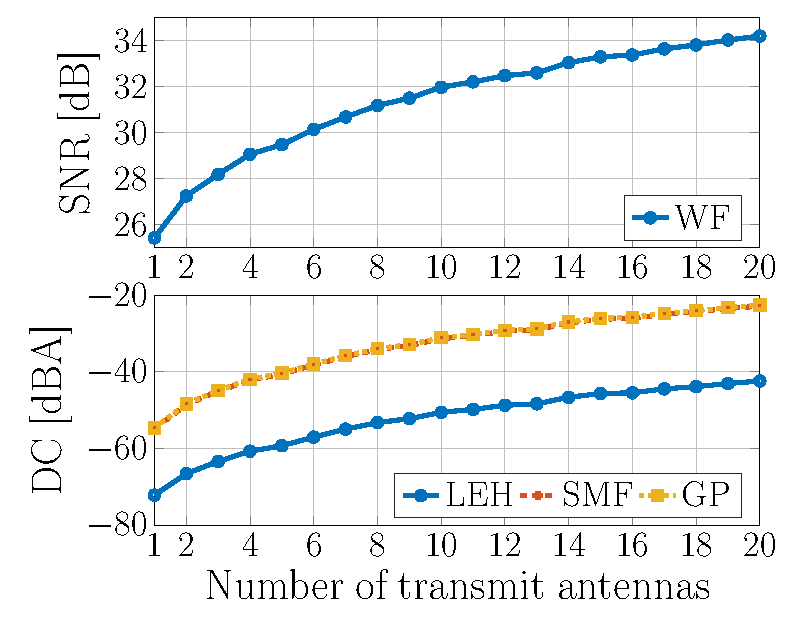
\includegraphics{assets/scaling_tx.eps}
				% This file was created by matlab2tikz.
%
%The latest updates can be retrieved from
%  http://www.mathworks.com/matlabcentral/fileexchange/22022-matlab2tikz-matlab2tikz
%where you can also make suggestions and rate matlab2tikz.
%
\definecolor{mycolor1}{rgb}{0.00000,0.44700,0.74100}%
\definecolor{mycolor2}{rgb}{0.85000,0.32500,0.09800}%
\definecolor{mycolor3}{rgb}{0.92900,0.69400,0.12500}%
%
\begin{tikzpicture}

\begin{axis}[%
width=4.036in,
height=1.531in,
at={(0.677in,2.323in)},
scale only axis,
xmin=1,
xmax=20,
xtick={ 1,  2,  4,  6,  8, 10, 12, 14, 16, 18, 20},
ymin=25,
ymax=35,
ylabel style={font=\color{white!15!black}},
ylabel={SNR [dB]},
axis background/.style={fill=white},
xmajorgrids,
ymajorgrids,
legend style={at={(0.97,0.03)}, anchor=south east, legend cell align=left, align=left, draw=white!15!black},
title style={font=\Large}, label style={font=\Large}, ticklabel style={font=\Large}, legend style={font=\Large}
]
\addplot [color=mycolor1, line width=2.0pt, mark=o, mark options={solid, mycolor1}]
  table[row sep=crcr]{%
1	25.4114090912701\\
2	27.2380228951407\\
3	28.1806581890125\\
4	29.0579705445501\\
5	29.4765358391588\\
6	30.1378186907448\\
7	30.679947158175\\
8	31.1807109572709\\
9	31.4989826016408\\
10	31.9754948092231\\
11	32.2100547605094\\
12	32.4793684081158\\
13	32.6017479139679\\
14	33.0455806994505\\
15	33.2977363152879\\
16	33.3793608838988\\
17	33.6454245558489\\
18	33.8188574644109\\
19	34.0296394451643\\
20	34.2013611372363\\
};
\addlegendentry{WF}

\end{axis}

\begin{axis}[%
width=4.036in,
height=1.531in,
at={(0.677in,0.472in)},
scale only axis,
xmin=1,
xmax=20,
xtick={ 1,  2,  4,  6,  8, 10, 12, 14, 16, 18, 20},
xlabel style={font=\color{white!15!black}},
xlabel={Number of transmit antennas},
ymin=-80,
ymax=-20,
ytick={-100,  -80,  -60,  -40,  -20,    0},
ylabel style={font=\color{white!15!black}},
ylabel={DC [dBA]},
axis background/.style={fill=white},
xmajorgrids,
ymajorgrids,
legend style={at={(0.97,0.03)}, anchor=south east, legend columns=3, legend cell align=left, align=left, draw=white!15!black},
title style={font=\Large}, label style={font=\Large}, ticklabel style={font=\Large}, legend style={font=\Large}
]
\addplot [color=mycolor1, line width=2.0pt, mark=o, mark options={solid, mycolor1}]
  table[row sep=crcr]{%
1	-72.1640311093757\\
2	-66.5715790324143\\
3	-63.3793292727081\\
4	-60.7012754464437\\
5	-59.266736864924\\
6	-57.0166388749873\\
7	-54.9404042138719\\
8	-53.2358069540989\\
9	-52.1931096939026\\
10	-50.5402642920901\\
11	-49.7737174862002\\
12	-48.6942616044043\\
13	-48.3135677149876\\
14	-46.6070871056972\\
15	-45.6179653081741\\
16	-45.4483986121797\\
17	-44.4091788705729\\
18	-43.8308588242839\\
19	-43.0166726001883\\
20	-42.3720905877998\\
};
\addlegendentry{LEH}

\addplot [color=mycolor2, dashed, line width=2.0pt, mark=+, mark options={solid, mycolor2}]
  table[row sep=crcr]{%
1	-54.8293278493535\\
2	-48.5800689706095\\
3	-45.0342330744972\\
4	-42.1572086079209\\
5	-40.5379337462381\\
6	-38.1993090160679\\
7	-35.9990333153406\\
8	-34.1537239955202\\
9	-33.0868304064636\\
10	-31.3112830269043\\
11	-30.4678953855246\\
12	-29.3603051671117\\
13	-28.9604248289287\\
14	-27.1704462396604\\
15	-26.214120462541\\
16	-25.9957086131491\\
17	-24.9246434665737\\
18	-24.2341851437915\\
19	-23.3987911541966\\
20	-22.801745202018\\
};
\addlegendentry{SMF}

\addplot [color=mycolor3, dotted, line width=2.0pt, mark=square, mark options={solid, mycolor3}]
  table[row sep=crcr]{%
1	-54.5941100581416\\
2	-48.3398061448139\\
3	-44.7929632074622\\
4	-41.9150112843405\\
5	-40.2926274936065\\
6	-37.9552739674627\\
7	-35.7534247682157\\
8	-33.9090703270243\\
9	-32.8415639562783\\
10	-31.0633765548807\\
11	-30.2229596446913\\
12	-29.1126774801063\\
13	-28.7130714340961\\
14	-26.9231116749848\\
15	-25.96807932327\\
16	-25.7475053662042\\
17	-24.6769859070682\\
18	-23.9860131480335\\
19	-23.1509323056183\\
20	-22.553989067624\\
};
\addlegendentry{GP}

\end{axis}
\end{tikzpicture}%

			}
		}
		\caption{Average \gls{r-e} region, \gls{wit} \gls{snr} and \gls{wpt} \gls{dc} versus $M$ for $N=16$, $L=20$, $\sigma_n^2=\qty{-40}{dBm}$, $B=\qty{1}{\MHz}$, $d_{\mathrm{H}}=d_{\mathrm{V}}=\qty{0.2}{\meter}$.}
	\end{figure}

	\begin{figure}[!t]
		\centering
		\subfloat[\gls{r-e} region\label{fi:re_reflector}]{
			\resizebox{0.425\columnwidth}{!}{
				% 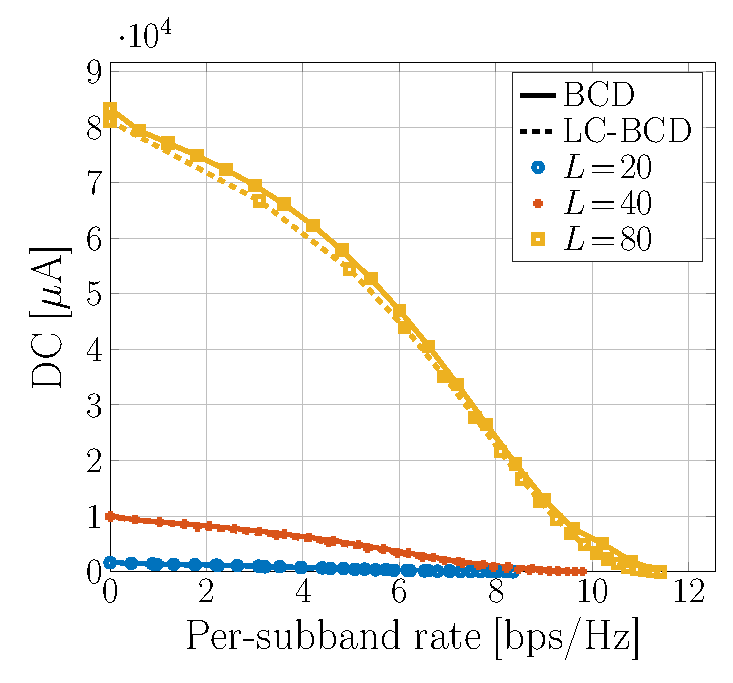
\includegraphics{assets/re_reflector.eps}
				% This file was created by matlab2tikz.
%
%The latest updates can be retrieved from
%  http://www.mathworks.com/matlabcentral/fileexchange/22022-matlab2tikz-matlab2tikz
%where you can also make suggestions and rate matlab2tikz.
%
\definecolor{mycolor1}{rgb}{0.00000,0.44706,0.74118}%
\definecolor{mycolor2}{rgb}{0.85098,0.32549,0.09804}%
\definecolor{mycolor3}{rgb}{0.92941,0.69412,0.12549}%
%
\begin{tikzpicture}

\begin{axis}[%
width=4.036in,
height=3.396in,
at={(0.677in,0.458in)},
scale only axis,
xmin=0,
xlabel style={font=\color{white!15!black}},
xlabel={Per-subband rate [bps/Hz]},
ymin=0,
ylabel style={font=\color{white!15!black}},
ylabel={DC [$\mu$A]},
axis background/.style={fill=white},
xmajorgrids,
ymajorgrids,
legend style={legend cell align=left, align=left, draw=white!15!black},
title style={font=\Large}, label style={font=\Large}, ticklabel style={font=\Large}, legend style={font=\Large}
]
\addplot [color=mycolor1, line width=2.0pt, mark=o, mark options={solid, mycolor1}, forget plot]
  table[row sep=crcr]{%
8.3586406696557	2.22044604925031e-10\\
7.91871221327587	35.983515390148\\
7.47878375703205	90.2593494563528\\
7.03885530082205	144.441595913417\\
6.59892684469334	190.366258147621\\
6.15899839068364	266.41995722542\\
5.71906993338534	362.975025961052\\
5.27914147582538	469.643413747422\\
4.83921301936429	581.156071268694\\
4.39928456310017	693.367239333508\\
3.95935610689076	803.167733985017\\
3.51942765064735	908.443493403437\\
3.07949919450721	1007.95741362605\\
2.6395707386736	1101.22921789342\\
2.19964228279862	1188.42108539005\\
1.75971383240915	1270.31846078728\\
1.31978553941413	1348.43370831148\\
0.879857419496064	1425.58310632458\\
0.43993218815602	1508.78146154449\\
1.19969027052e-09	1671.11145229677\\
};
\addplot [color=mycolor1, dashed, line width=2.0pt, mark=o, mark options={solid, mycolor1}, forget plot]
  table[row sep=crcr]{%
8.35864066965403	2.22044604925031e-10\\
8.20294090351821	3.41667296364854\\
8.03862919172743	8.59523165459973\\
7.86443923165709	15.8933140672386\\
7.67911929886492	25.9043164830599\\
7.48116073897242	39.4573504949537\\
7.2687229851279	57.6172252527604\\
7.03953660784295	81.6844368554499\\
6.79075709918349	113.195156306034\\
6.51875740157038	153.921271425166\\
6.21881593690335	205.870335406696\\
5.88463594859029	271.2856475107\\
5.50757623951716	352.646182425718\\
5.07536948872174	452.66665040299\\
4.56987969239559	574.297488236912\\
3.96301635795142	720.724829144859\\
3.20922959563788	895.370547654322\\
2.23465212090367	1101.8922204845\\
0.967425742530333	1344.18317602786\\
0	1626.37239654442\\
};
\addplot [color=mycolor2, line width=2.0pt, mark=+, mark options={solid, mycolor2}, forget plot]
  table[row sep=crcr]{%
9.7976374608085	2.22044604925031e-10\\
9.28197233121829	209.7166267373\\
8.76630720175656	555.051261375093\\
8.25064207229597	888.316833899828\\
7.73497694277984	1271.90000290159\\
7.21931181324324	1892.07747881737\\
6.70364668373293	2603.99344622679\\
6.18798155425005	3359.82095005772\\
5.67231642481146	4120.87427527931\\
5.15665129537383	4858.46068011754\\
4.64098616586208	5553.52518097301\\
4.12532103660684	6195.25099208548\\
3.60965590728052	6779.31472556579\\
3.09399077778669	7306.27090357847\\
2.57832564836549	7780.24169889972\\
2.06266051899262	8208.30341411677\\
1.54699538943343	8600.52759222459\\
1.03133026259681	8972.41199145399\\
0.515665416218068	9356.13399043515\\
3.68430926817684e-11	10067.7549388996\\
};
\addplot [color=mycolor2, dashed, line width=2.0pt, mark=+, mark options={solid, mycolor2}, forget plot]
  table[row sep=crcr]{%
9.79763745852635	2.22044604925031e-10\\
9.64176922686156	11.7387455736164\\
9.47706252125669	34.269724508739\\
9.30239747700265	69.7760176214405\\
9.11649563574005	121.888493683525\\
8.91781523457799	195.685727191512\\
8.70447344351968	297.69397303328\\
8.47413948258538	435.887073499262\\
8.22387994437141	619.686502266237\\
7.94993139648082	859.961361632274\\
7.64735850808491	1169.02840729544\\
7.30951383829502	1560.6520050723\\
6.92714604650855	2050.04423769427\\
6.48685391190609	2653.86482651954\\
5.96820459636463	3390.2212468847\\
5.33790028361791	4278.66855492454\\
4.53663782338788	5340.20947011474\\
3.445737967756	6597.29452625595\\
1.80700925547565	8073.82195534215\\
0	9795.13734580782\\
};
\addplot [color=mycolor3, line width=2.0pt, mark=square, mark options={solid, mycolor3}, forget plot]
  table[row sep=crcr]{%
11.4122579700926	2.22044604925031e-10\\
10.811612813709	1898.58408147828\\
10.210967657439	5069.50599004224\\
9.61032250114462	7762.226632269\\
9.00967734480262	12946.1927394065\\
8.40903218848343	19401.9636925237\\
7.80838703220193	26472.5398330781\\
7.20774187603675	33649.1750044694\\
6.60709671969197	40559.6943368711\\
6.00645156345879	46966.837734146\\
5.40580640760185	52745.625695835\\
4.80516125120929	57854.4542860969\\
4.20451609506615	62308.3755596472\\
3.60387093904179	66158.0539714355\\
3.00322578280851	69474.9813830017\\
2.40258062657304	72343.297600595\\
1.80193547015798	74857.6300896923\\
1.20129031461481	77135.6998951966\\
0.600645164346655	79377.1510569523\\
2.85327610786461e-13	83298.7244267066\\
};
\addplot [color=mycolor3, dashed, line width=2.0pt, mark=square, mark options={solid, mycolor3}, forget plot]
  table[row sep=crcr]{%
11.4122579636798	2.22044604925031e-10\\
11.256294973482	61.9298284449408\\
11.0914394573555	213.843902697059\\
10.9165962128431	473.921069561986\\
10.7304776524065	872.431766352402\\
10.5315300482826	1451.73788456734\\
10.3178546840706	2266.29265847508\\
10.0870973533826	3382.64058670426\\
9.83629062260695	4879.41740229352\\
9.5616206072301	6847.34984197071\\
9.25807134937778	9389.25585277989\\
8.91886133846138	12620.0449149525\\
8.53450540575679	16666.7174382927\\
8.09115990871213	21668.3648887966\\
7.56747593290251	27776.1701058218\\
6.92800012657884	35153.407106665\\
6.10734222403926	43975.4415609724\\
4.96397265607329	54429.7305026897\\
3.09913335958453	66715.8208782246\\
0	81045.3520467765\\
};
\addplot [color=black, line width=2.0pt]
  table[row sep=crcr]{%
-1	-1\\
};
\addlegendentry{BCD}

\addplot [color=black, dashed, line width=2.0pt]
  table[row sep=crcr]{%
-1	-1\\
};
\addlegendentry{LC-BCD}

\addplot [color=mycolor1, line width=2.0pt, only marks, mark=o, mark options={solid, mycolor1}]
  table[row sep=crcr]{%
-1	-1\\
};
\addlegendentry{$L = 20$}

\addplot [color=mycolor2, line width=2.0pt, only marks, mark=+, mark options={solid, mycolor2}]
  table[row sep=crcr]{%
-1	-1\\
};
\addlegendentry{$L = 40$}

\addplot [color=mycolor3, line width=2.0pt, only marks, mark=square, mark options={solid, mycolor3}]
  table[row sep=crcr]{%
-1	-1\\
};
\addlegendentry{$L = 80$}

\end{axis}
\end{tikzpicture}%

			}
		}
		\subfloat[\gls{wit} \gls{snr} and \gls{wpt} \gls{dc}\label{fi:scaling_reflector}]{
			\resizebox{0.475\columnwidth}{!}{
				% 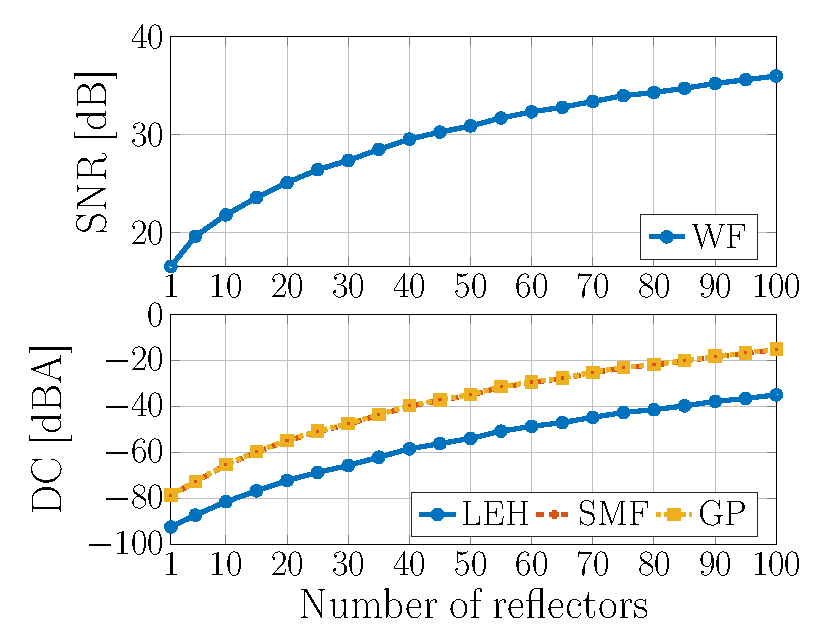
\includegraphics{assets/scaling_reflector.eps}
				% This file was created by matlab2tikz.
%
%The latest updates can be retrieved from
%  http://www.mathworks.com/matlabcentral/fileexchange/22022-matlab2tikz-matlab2tikz
%where you can also make suggestions and rate matlab2tikz.
%
\definecolor{mycolor1}{rgb}{0.00000,0.44700,0.74100}%
\definecolor{mycolor2}{rgb}{0.85000,0.32500,0.09800}%
\definecolor{mycolor3}{rgb}{0.92900,0.69400,0.12500}%
%
\begin{tikzpicture}

\begin{axis}[%
width=4.036in,
height=1.531in,
at={(0.677in,2.323in)},
scale only axis,
xmin=1,
xmax=100,
xtick={  1,  10,  20,  30,  40,  50,  60,  70,  80,  90, 100},
ymin=16.5555734490246,
ymax=40,
ylabel style={font=\color{white!15!black}},
ylabel={SNR [dB]},
axis background/.style={fill=white},
xmajorgrids,
ymajorgrids,
legend style={at={(0.97,0.03)}, anchor=south east, legend cell align=left, align=left, draw=white!15!black},
title style={font=\huge}, label style={font=\huge}, ticklabel style={font=\LARGE}, legend style={font=\LARGE}
]
\addplot [color=mycolor1, line width=2.0pt, mark=o, mark options={solid, mycolor1}]
  table[row sep=crcr]{%
1	16.5555734490246\\
5	19.6335595133498\\
10	21.8178579734798\\
15	23.5761671596729\\
20	25.1046157566153\\
25	26.4353009128835\\
30	27.3687767493369\\
35	28.5000247501475\\
40	29.55470011095\\
45	30.2660500078313\\
50	30.8940169652101\\
55	31.7135354369005\\
60	32.341170905938\\
65	32.8036703248563\\
70	33.3976115406002\\
75	33.9866791914948\\
80	34.3153022204229\\
85	34.7478623486695\\
90	35.2274340968895\\
95	35.6119521148845\\
100	35.9998760976194\\
};
\addlegendentry{WF}

\end{axis}

\begin{axis}[%
width=4.036in,
height=1.531in,
at={(0.677in,0.472in)},
scale only axis,
xmin=1,
xmax=100,
xtick={  1,  10,  20,  30,  40,  50,  60,  70,  80,  90, 100},
xlabel style={font=\color{white!15!black}},
xlabel={Number of reflectors},
ymin=-100,
ymax=0,
ytick={-100,  -80,  -60,  -40,  -20,    0},
ylabel style={font=\color{white!15!black}},
ylabel={DC [dBA]},
axis background/.style={fill=white},
xmajorgrids,
ymajorgrids,
legend style={at={(0.97,0.03)}, anchor=south east, legend columns=3, legend cell align=left, align=left, draw=white!15!black},
title style={font=\huge}, label style={font=\huge}, ticklabel style={font=\LARGE}, legend style={font=\LARGE}
]
\addplot [color=mycolor1, line width=2.0pt, mark=o, mark options={solid, mycolor1}]
  table[row sep=crcr]{%
1	-92.5536970513039\\
5	-87.4040857061315\\
10	-81.5588189562214\\
15	-76.8140292111448\\
20	-72.3119132681356\\
25	-68.7912416779769\\
30	-65.7862313987141\\
35	-62.1723146529388\\
40	-58.5241681973142\\
45	-56.2591989620605\\
50	-53.9864632003429\\
55	-50.8433722019956\\
60	-48.7348538385412\\
65	-47.0991935158248\\
70	-44.8084149592399\\
75	-42.6836629529512\\
80	-41.4931625063164\\
85	-39.8213975436717\\
90	-37.8873698523974\\
95	-36.6019945477592\\
100	-35.0270512662257\\
};
\addlegendentry{LEH}

\addplot [color=mycolor2, dashed, line width=2.0pt, mark=+, mark options={solid, mycolor2}]
  table[row sep=crcr]{%
1	-78.9404966300438\\
5	-72.8653842234958\\
10	-65.561806372763\\
15	-60.0355415823876\\
20	-55.0277956057781\\
25	-51.0918624499135\\
30	-47.829959033523\\
35	-43.8800207934611\\
40	-39.9870037432698\\
45	-37.4246355658198\\
50	-35.09156159735\\
55	-31.7254806484209\\
60	-29.6556112190413\\
65	-27.9027388534924\\
70	-25.4289617613286\\
75	-23.32558330701\\
80	-22.0667156512475\\
85	-20.3765921162739\\
90	-18.4192057525797\\
95	-16.9836370754222\\
100	-15.3684103792823\\
};
\addlegendentry{SMF}

\addplot [color=mycolor3, dotted, line width=2.0pt, mark=square, mark options={solid, mycolor3}]
  table[row sep=crcr]{%
1	-78.711551303767\\
5	-72.6351143679569\\
10	-65.3278838246729\\
15	-59.7998504435555\\
20	-54.791570853135\\
25	-50.8545605551382\\
30	-47.5929011664101\\
35	-43.6415675742364\\
40	-39.7487995240244\\
45	-37.1874794473846\\
50	-34.8530261281813\\
55	-31.4884244381754\\
60	-29.4174064918624\\
65	-27.6650993474425\\
70	-25.1913292817342\\
75	-23.0883653237371\\
80	-21.8292565432622\\
85	-20.1391870609115\\
90	-18.1812656012089\\
95	-16.7459125238822\\
100	-15.1306956073902\\
};
\addlegendentry{GP}

\end{axis}
\end{tikzpicture}%
			}
		}
		\caption{Average \gls{r-e} region, \gls{wit} \gls{snr} and \gls{wpt} \gls{dc} versus $L$ for $M=1$, $N=16$, $\sigma_n^2=\qty{-40}{dBm}$, $B=\qty{1}{\MHz}$ and $d_{\mathrm{H}}=d_{\mathrm{V}}=\qty{0.2}{\meter}$.}
	\end{figure}

	The impacts of the number of transmit antennas $M$ and the \gls{ris} elements $L$ on the \gls{r-e} behavior are revealed in Figs.~\subref*{fi:re_tx} and \subref*{fi:re_reflector}. First, it is observed that adding either active or passive elements can improve the equivalent \gls{snr}, which produces a nearly concave \gls{r-e} region and favors the \gls{ps} receiver. Second, the conventional Linear Energy Harvester (LEH) model leads to a power-inefficient design. To investigate the performance loss, we truncate the \gls{dc} objective function \eqref{eq:z} at $n_0=2$ such that (i) in the passive beamforming problem, $z(\boldsymbol{\Phi}) = {\beta_2}{\rho}(t_{\mathrm{I},0}+t_{\mathrm{P},0})/2$ and no \gls{sca} is required; (ii) in the waveform design problem, the \gls{wpt}-optimal strategy is the adaptive single sinewave that allocates all power to the multisine at the strongest subband \cite{Clerckx2016a}. As shown in Figs.~\subref*{fi:scaling_tx} and \subref*{fi:scaling_reflector}, those conventional designs do not exploit the harvester nonlinearity and end up with a nearly \qty{20}{dBA} gap compared to the nonlinear model-based \gls{smf} and \gls{gp} designs. Third, doubling $M$ brings a \qty{3}{\dB} gain at the output \gls{snr} and a \qty{12}{dBA} increase at the harvested \gls{dc}, which verified that active beamforming has an array gain of $M$ \cite{Tse2005} with power scaling order $M^2$ under the truncated nonlinear harvester model \cite{Clerckx2016a,Clerckx2018b}. Fourth, when the \gls{ris} is very close to the \gls{ap} or \gls{ue}, doubling $L$ can bring a \qty{6}{\dB} gain at the output \gls{snr} and a \qty{24}{dBA} increase at the harvested \gls{dc}. From the perspective of \gls{wit}, it suggests that passive beamforming can reach an array gain of $L^2$, as indicated by \cite{Wu2019}. An interpretation is that the \gls{ris} coherently combines the incoming signal with a receive array gain $L$, then performs an equal gain reflection with a transmit array gain $L$. From the perspective of \gls{wpt}, it suggests that passive beamforming comes with a power scaling order $L^4$ under the truncated nonlinear harvester model. We then verify this novel observation in a simplified case where the power is uniformly allocated over multisine, all channels are frequency-flat, and $L$ is sufficiently large such that the direct channel becomes negligible. Let $X$ be the cascaded small-scale fading coefficient. The \gls{dc} in such case reduces to
	\begin{equation}
		z = \beta_2 \Lambda_{\mathrm{R}}^2 \Lambda_{\mathrm{I}}^2 \lvert X \rvert^2 L^2 P + \beta_4 \frac{2N^2 + 1}{2N} \Lambda_{\mathrm{R}}^4 \Lambda_{\mathrm{I}}^4 \lvert X \rvert^4 L^4 P^2,
	\end{equation}
	which scales quartically with $L$. Compared with active antennas, \gls{ris} elements achieve higher array gain and power scaling order, but a very large $L$ is required to compensate the double fading of the auxiliary link. These observations demonstrate the \gls{r-e} benefit of passive beamforming and emphasize the importance of accounting for the harvester nonlinearity in the waveform and beamforming design.

	\begin{figure}[!t]
		\centering
		\subfloat[$B=\qty{1}{\MHz}$\label{fi:re_irs_1mhz}]{
			\resizebox{0.45\columnwidth}{!}{
				% 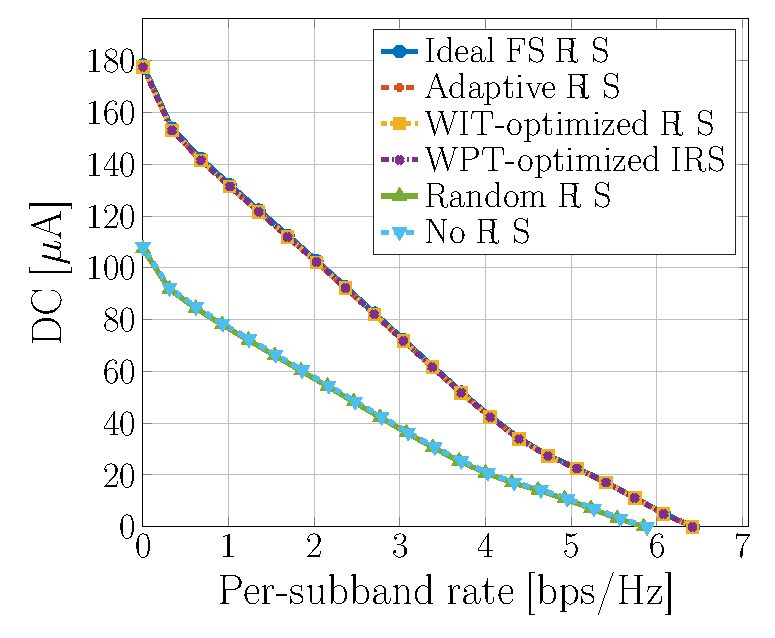
\includegraphics{assets/re_irs_1mhz.eps}
				% This file was created by matlab2tikz.
%
%The latest updates can be retrieved from
%  http://www.mathworks.com/matlabcentral/fileexchange/22022-matlab2tikz-matlab2tikz
%where you can also make suggestions and rate matlab2tikz.
%
\definecolor{mycolor1}{rgb}{0.00000,0.44700,0.74100}%
\definecolor{mycolor2}{rgb}{0.85000,0.32500,0.09800}%
\definecolor{mycolor3}{rgb}{0.92900,0.69400,0.12500}%
\definecolor{mycolor4}{rgb}{0.49400,0.18400,0.55600}%
\definecolor{mycolor5}{rgb}{0.46600,0.67400,0.18800}%
\definecolor{mycolor6}{rgb}{0.30100,0.74500,0.93300}%
%
\begin{tikzpicture}

\begin{axis}[%
width=4.036in,
height=3.387in,
at={(0.677in,0.457in)},
scale only axis,
xmin=0,
xlabel style={font=\color{white!15!black}},
xlabel={Per-subband rate [bps/Hz]},
ymin=0,
ylabel style={font=\color{white!15!black}},
ylabel={DC [$\mu$A]},
axis background/.style={fill=white},
xmajorgrids,
ymajorgrids,
legend style={legend cell align=left, align=left, draw=white!15!black},
title style={font=\huge}, label style={font=\huge}, ticklabel style={font=\LARGE}, legend style={font=\LARGE}
]
\addplot [color=mycolor1, line width=2.0pt, mark=o, mark options={solid, mycolor1}]
  table[row sep=crcr]{%
6.4253320699697	0\\
6.08715672384594	5.01108258373026\\
5.74898175436141	11.1464906078818\\
5.41080647103305	17.1839306901179\\
5.07263119587457	22.6007781742555\\
4.73445701681299	27.4632098259609\\
4.39628185051099	34.0809981751516\\
4.05810690956665	42.5661420810435\\
3.71993220475979	52.0019060060565\\
3.38175841319093	61.9658849905797\\
3.04358524881016	72.1917317246937\\
2.70541369690409	82.4700244716243\\
2.3672401476998	92.6614580137511\\
2.02906325064618	102.688839356222\\
1.69088759747245	112.534965851474\\
1.35271356837879	122.259405107842\\
1.01454659162539	132.026221643851\\
0.676395709790915	142.218501584658\\
0.338243915647267	153.877063062521\\
1.4851638963565e-06	178.353328355518\\
};
\addlegendentry{Ideal FS RIS}

\addplot [color=mycolor2, dashed, line width=2.0pt, mark=+, mark options={solid, mycolor2}]
  table[row sep=crcr]{%
6.41709023569077	2.22044604925031e-10\\
6.07934864438239	4.98570407847135\\
5.7416070645871	11.0875128283569\\
5.40386549531567	17.0907440501218\\
5.0661239437523	22.4786432816181\\
4.72838260626359	27.3163184986736\\
4.39064086877545	33.956504428874\\
4.05289942739781	42.3412746282033\\
3.71515810616043	51.7255137417252\\
3.37741702450112	61.6473815290737\\
3.03967767692813	71.8111084899675\\
2.70193688940078	82.0391505440427\\
2.36419501626497	92.1818377589969\\
2.02645293926653	102.162122990288\\
1.68871023752978	111.965723128668\\
1.3509687750037	121.650568582524\\
1.01322788210054	131.381574723619\\
0.675498531405969	141.528732622007\\
0.337779870999036	153.144903892215\\
1.77342843727211e-07	177.521232964326\\
};
\addlegendentry{Adaptive RIS}

\addplot [color=mycolor3, dotted, line width=2.0pt, mark=square, mark options={solid, mycolor3}]
  table[row sep=crcr]{%
6.41709023569077	0\\
6.07934867262404	4.98435310995074\\
5.74160751512904	11.0839114024536\\
5.40386601195288	17.085025314706\\
5.06612452078785	22.4684009770537\\
4.72838422458933	27.3017723005741\\
4.39064287139896	33.8899437071872\\
4.05290179732597	42.3302887410965\\
3.71516111488971	51.7160814509496\\
3.37742139791828	61.6293110402637\\
3.03968248223031	71.8026940320553\\
2.70194553428282	82.0290573352337\\
2.36420497066294	92.1702603982497\\
2.0264625888992	102.148712150631\\
1.68871860697363	111.948869028923\\
1.35097999533801	121.627918920384\\
1.01324909865069	131.351598493342\\
0.67552871453759	141.500089224442\\
0.337811215101083	153.108996199914\\
1.48078416642661e-06	177.488565146194\\
};
\addlegendentry{WIT-optimized RIS}

\addplot [color=mycolor4, dashdotted, line width=2.0pt, mark=x, mark options={solid, mycolor4}]
  table[row sep=crcr]{%
6.41628377550057	0\\
6.0785846630055	4.9844503501816\\
5.74088601445629	11.0846440558454\\
5.40318695458732	17.0871778462167\\
5.06548790583293	22.472904256829\\
4.72778893784929	27.3095493481099\\
4.3900912730883	33.8967634035481\\
4.0523927230224	42.3378093870174\\
3.71469466818064	51.7246825743966\\
3.37699782381373	61.6391682668772\\
3.03930192964141	71.8139337609969\\
2.70160563217874	82.0421443865812\\
2.36390866581197	92.1846182987774\\
2.02620787709825	102.164720140442\\
1.68850621991026	111.966608461958\\
1.35081034070007	121.647505669315\\
1.01312176326262	131.373158855128\\
0.675444821842704	141.524109434005\\
0.337770416130866	153.136633336489\\
1.48488440575836e-06	177.513391721269\\
};
\addlegendentry{WPT-optimized RIS}

\addplot [color=mycolor5, line width=2.0pt, mark=triangle, mark options={solid, mycolor5}]
  table[row sep=crcr]{%
5.84439697467332	0\\
5.53679827244144	3.26861703702415\\
5.22920256954895	7.09220530725155\\
4.92160471884745	10.8234655569083\\
4.6140178419029	14.1797038200929\\
4.30641880625976	17.0203072237173\\
3.99883732175232	20.8236110313297\\
3.69123663501329	25.3598099138529\\
3.383656326501	30.6704115771568\\
3.07605207008533	36.3505688094805\\
2.76846482343931	42.2628416826838\\
2.4608784780121	48.2633474124216\\
2.15327005573453	54.2704043935467\\
1.84568510004087	60.2394071589979\\
1.53809277980483	66.1622828215739\\
1.23050552099583	72.0747123653626\\
0.922907234280382	78.081033263145\\
0.615316152044504	84.4214351312023\\
0.307735586791591	91.7631014737018\\
1.14919081261473e-05	107.386419697097\\
};
\addlegendentry{Random RIS}

\addplot [color=mycolor6, dashed, line width=2.0pt, mark=triangle, mark options={solid, rotate=180, mycolor6}]
  table[row sep=crcr]{%
5.88407124369286	0\\
5.57438389995066	3.29515031848895\\
5.26470100272104	7.1452898063542\\
4.95501325469587	10.9016346819385\\
4.64533517628943	14.2819928366442\\
4.33564589513226	17.1385183682365\\
4.02597177121309	20.9187345716662\\
3.7162836243057	25.4767376231786\\
3.40661331559676	30.8150358353255\\
3.09692637001789	36.5310006894027\\
2.7872378917577	42.4736244906829\\
2.47755963834982	48.5062242057831\\
2.16787349711756	54.5466904481599\\
1.85820673287037	60.5519858111177\\
1.54852110231338	66.5134696091136\\
1.23884447587655	72.4662996149154\\
0.929150550064657	78.5154060336347\\
0.619468349437254	84.9028447295244\\
0.309802813280014	92.3023593922935\\
1.30329138899424e-05	108.053363669481\\
};
\addlegendentry{No RIS}

\end{axis}
\end{tikzpicture}%

			}
		}
		\subfloat[$B=\qty{10}{\MHz}$\label{fi:re_irs_10mhz}]{
			\resizebox{0.45\columnwidth}{!}{
				% 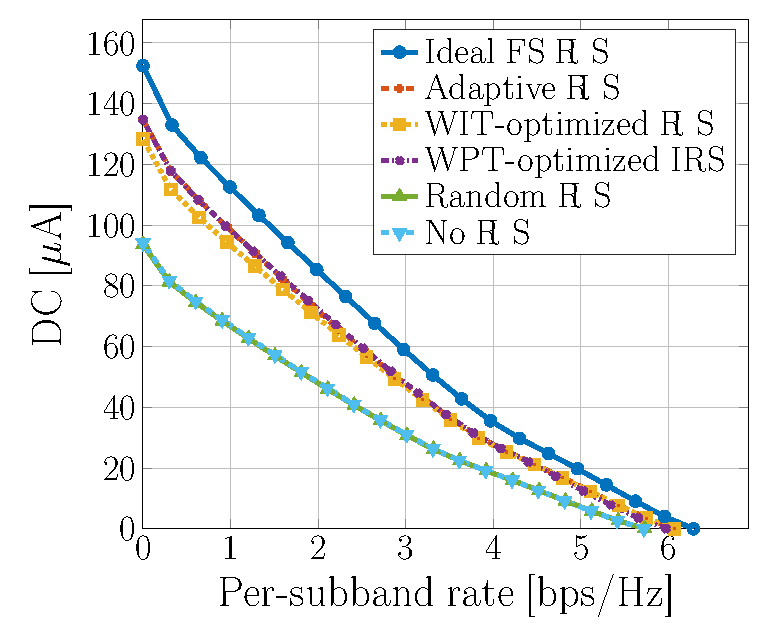
\includegraphics{assets/re_irs_10mhz.eps}
				% This file was created by matlab2tikz.
%
%The latest updates can be retrieved from
%  http://www.mathworks.com/matlabcentral/fileexchange/22022-matlab2tikz-matlab2tikz
%where you can also make suggestions and rate matlab2tikz.
%
\definecolor{mycolor1}{rgb}{0.00000,0.44700,0.74100}%
\definecolor{mycolor2}{rgb}{0.85000,0.32500,0.09800}%
\definecolor{mycolor3}{rgb}{0.92900,0.69400,0.12500}%
\definecolor{mycolor4}{rgb}{0.49400,0.18400,0.55600}%
\definecolor{mycolor5}{rgb}{0.46600,0.67400,0.18800}%
\definecolor{mycolor6}{rgb}{0.30100,0.74500,0.93300}%
%
\begin{tikzpicture}

\begin{axis}[%
width=4.036in,
height=3.396in,
at={(0.677in,0.458in)},
scale only axis,
xmin=0,
xlabel style={font=\color{white!15!black}},
xlabel={Per-subband rate [bps/Hz]},
ymin=0,
ylabel style={font=\color{white!15!black}},
ylabel={DC [$\mu$A]},
axis background/.style={fill=white},
xmajorgrids,
ymajorgrids,
legend style={legend cell align=left, align=left, draw=white!15!black},
title style={font=\Large}, label style={font=\Large}, ticklabel style={font=\Large}, legend style={font=\Large}
]
\addplot [color=mycolor1, line width=2.0pt, mark=o, mark options={solid, mycolor1}]
  table[row sep=crcr]{%
6.28562473551246	0\\
5.95480245026279	4.06626401518917\\
5.62398013942514	9.08714702489296\\
5.29315789306667	14.4253375590631\\
4.96233569456656	19.7631411179944\\
4.6315132725818	24.8296271801109\\
4.30069132448512	29.7894791166605\\
3.9698694783345	35.5494273522397\\
3.63904782649677	42.7962001711017\\
3.3082315298633	50.6527708249335\\
2.97741428013604	59.0552173236146\\
2.6466013260116	67.695118269391\\
2.31579084465345	76.4664632749714\\
1.98498439040319	85.3101410462159\\
1.65418120675299	94.2269926495056\\
1.32339084330662	103.265717078052\\
0.99258395700271	112.533300604385\\
0.66176958437251	122.187540856545\\
0.330932188395868	132.93781819835\\
4.04285284210013e-05	152.511750381353\\
};
\addlegendentry{Ideal FS RIS}

\addplot [color=mycolor2, dashed, line width=2.0pt, mark=+, mark options={solid, mycolor2}]
  table[row sep=crcr]{%
6.06950710388042	2.22044604925031e-10\\
5.75005936593249	3.49412040344887\\
5.43061163237636	7.7525003415335\\
5.11116393777849	12.2922177615999\\
4.79171645804167	16.8664364460734\\
4.47227279802113	21.3748843168415\\
4.15282246794847	25.563655117426\\
3.83337597089205	30.3723067979512\\
3.51392816619359	36.4222070922184\\
3.19448149970705	43.2236979001791\\
2.87503597822865	50.3711670396419\\
2.55559694033071	57.8632615879492\\
2.2361447509025	65.7339226680685\\
1.91669763814863	73.9012069742914\\
1.59725160997827	82.2514405133591\\
1.27780882741432	90.8501264759089\\
0.958370470323101	99.4417190837898\\
0.638927766755116	108.250341195861\\
0.31948617470048	117.828528430894\\
3.32882882477938e-05	134.757777758761\\
};
\addlegendentry{Adaptive RIS}

\addplot [color=mycolor3, dotted, line width=2.0pt, mark=square, mark options={solid, mycolor3}]
  table[row sep=crcr]{%
6.06950710388042	0\\
5.7500595455561	3.49018815155323\\
5.43061192596518	7.73791507212927\\
5.11116484698597	12.2494381082239\\
4.79171705093457	16.7746877033354\\
4.47226957471169	21.1935831820712\\
4.15282280483278	25.2763331438805\\
3.83337835216112	29.8388018117037\\
3.51393215446598	35.8868527630905\\
3.19448627172202	42.4665164803282\\
2.87506196757857	49.3432338162299\\
2.55563181725298	56.5389891245671\\
2.23620394794825	63.8253650502373\\
1.91677050603598	71.2749293413951\\
1.59733301822566	78.8181183475493\\
1.27791149320492	86.4997353415022\\
0.958465962104472	94.3808994896647\\
0.639012365735811	102.593415430155\\
0.319558027397639	111.724900246193\\
0.000107081360268932	128.380314721217\\
};
\addlegendentry{WIT-optimized RIS}

\addplot [color=mycolor4, dashdotted, line width=2.0pt, mark=x, mark options={solid, mycolor4}]
  table[row sep=crcr]{%
5.97367341463907	0\\
5.65927009123731	3.5070264102203\\
5.34486814850275	7.84528745241586\\
5.03046561323205	12.5383794438612\\
4.71606582426966	17.3267357303614\\
4.40166417994967	22.077858824616\\
4.08726063412393	26.4508055780473\\
3.7728545096199	31.522775063162\\
3.45845043759913	37.6436154195068\\
3.14405097462048	44.6133812899949\\
2.82966174581073	51.849933526765\\
2.51528366811897	59.4307178132691\\
2.20089691467726	67.2557740817545\\
1.88651119350457	75.2043023004085\\
1.57210835387927	83.2663359757171\\
1.2577214356617	91.4594403139737\\
0.943319951000214	99.7855218504222\\
0.628906066370186	108.399250259017\\
0.314493398574557	117.879771557813\\
8.55033452407821e-05	134.745174710166\\
};
\addlegendentry{WPT-optimized RIS}

\addplot [color=mycolor5, line width=2.0pt, mark=triangle, mark options={solid, mycolor5}]
  table[row sep=crcr]{%
5.72918734750297	0\\
5.42765153299674	2.67096293826227\\
5.12611639923297	5.83538639111985\\
4.82458063043276	9.19527763613911\\
4.52304523948057	12.5944230500271\\
4.22151117299483	15.9532889145451\\
3.9199787922983	19.0939383517133\\
3.61844839682222	22.4331431170865\\
3.31691871489426	26.195529954522\\
3.01538774223012	30.7688509835499\\
2.71385794634512	35.6490224895363\\
2.41234093734843	40.7053860595845\\
2.11083149721089	46.001422884172\\
1.80932674489596	51.4296433875211\\
1.50781501926691	56.9919580345752\\
1.20628195171052	62.6684266820058\\
0.904758598926291	68.4737591137524\\
0.603224626752544	74.5505599184922\\
0.301666573662066	81.3192960640207\\
3.183219975178e-06	93.6399496572079\\
};
\addlegendentry{Random RIS}

\addplot [color=mycolor6, dashed, line width=2.0pt, mark=triangle, mark options={solid, rotate=180, mycolor6}]
  table[row sep=crcr]{%
5.71979443964052	0\\
5.41875304408695	2.67919296158555\\
5.11771317004337	5.85700253185807\\
4.81667267672687	9.23237896525134\\
4.5156331203365	12.6476434772588\\
4.21459439402178	16.0243487841886\\
3.91355618152882	19.1827877194726\\
3.61251879288058	22.5818095535712\\
3.31148338886151	26.352385210698\\
3.01044248590787	31.0294471416115\\
2.709410575653	35.8886400393912\\
2.40838490553982	40.9995850388112\\
2.10739419995416	46.3037406401343\\
1.80637864180582	51.7117925666906\\
1.5053639005762	57.2966131068832\\
1.20431563278455	62.9970251769627\\
0.903274595029508	68.8326808177523\\
0.602227456298545	74.9498973122969\\
0.301161803909952	81.768808211141\\
3.17118565621855e-06	94.1282050990962\\
};
\addlegendentry{No RIS}

\end{axis}
\end{tikzpicture}%

			}
		}
		\caption{Average \gls{r-e} region for ideal, adaptive, fixed and no \gls{ris} versus $B$ for $M=1$, $N=16$, $L=20$, $\sigma_n^2=\qty{-40}{dBm}$ and $d_{\mathrm{H}}=d_{\mathrm{V}}=\qty{2}{\meter}$.}
	\end{figure}

	Figs.~\subref*{fi:re_irs_1mhz} and \subref*{fi:re_irs_10mhz} explore the \gls{r-e} region with different \gls{ris} strategies for narrowband and broadband \gls{swipt}. The ideal Frequency-Selective (FS) \gls{ris} assumes the reflection coefficient of each element is independent and controllable at different frequencies. The adaptive \gls{ris} adjusts the passive beamforming for different \gls{r-e} points by Algorithm~\ref{al:sca}. The \gls{wit}/\gls{wpt}-optimized \gls{ris} is retrieved by Algorithm~\ref{al:m_sca} then fixed for the whole \gls{r-e} region. The random \gls{ris} models the phase shift of all elements as i.i.d. uniform random variables over $[0, 2\pi)$. First, random \gls{ris} and no \gls{ris} perform worse than other schemes since no passive beamforming is exploited. Their \gls{r-e} boundaries coincide as the antenna mode reflection of the random \gls{ris} is canceled out after averaging. Second, when the bandwidth is small, the performance of ideal, adaptive, and \gls{wit}/\gls{wpt}-optimized \gls{ris} are similar; when the bandwidth is large, the adaptive \gls{ris} outperforms the \gls{wit}/\gls{wpt}-optimized \gls{ris} but is outperformed by the ideal FS \gls{ris}. In the former case, the subband responses are close to each other such that the tradeoff in Remark~\ref{re:subband_tradeoff} becomes insignificant, and the auxiliary link can be roughly maximized at all subbands. It suggests that for narrowband \gls{swipt}, the optimal passive beamforming for any \gls{r-e} point is optimal for the whole \gls{r-e} region, and the corresponding composite channel and active precoder are also optimal for the whole \gls{r-e} region. Hence, the achievable \gls{r-e} region is obtained by optimizing the waveform amplitude and splitting ratio. On the other hand, since the channel frequency selectivity affects the performance of the information decoder and energy harvester differently, the optimal \gls{ris} reflection coefficient varies at different \gls{r-e} tradeoffs points for broadband \gls{swipt}. As shown in Fig.~\ref{fi:channel_amplitude}, the subchannel amplification can be either spread evenly to improve the rate at high \gls{snr}, or focused on a few strongest subbands to boost the output \gls{dc}, thanks to adaptive passive beamforming.

	\begin{figure}[!t]
		\centering
		\subfloat[Imperfect cascaded \gls{csit}\label{fi:re_csi}]{
			\resizebox{0.45\columnwidth}{!}{
				% 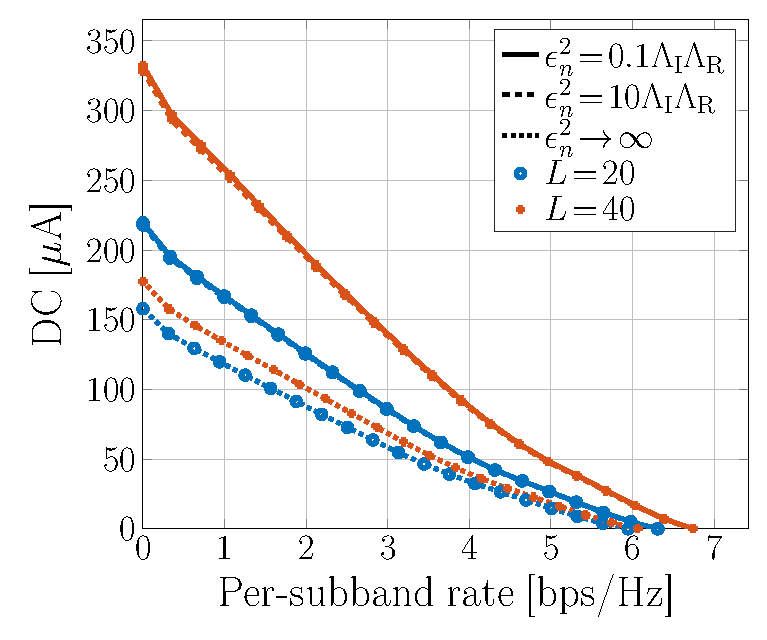
\includegraphics{assets/re_csi.eps}
				% This file was created by matlab2tikz.
%
%The latest updates can be retrieved from
%  http://www.mathworks.com/matlabcentral/fileexchange/22022-matlab2tikz-matlab2tikz
%where you can also make suggestions and rate matlab2tikz.
%
\definecolor{mycolor1}{rgb}{0.00000,0.44706,0.74118}%
\definecolor{mycolor2}{rgb}{0.85098,0.32549,0.09804}%
%
\begin{tikzpicture}

\begin{axis}[%
width=4.036in,
height=3.396in,
at={(0.677in,0.458in)},
scale only axis,
xmin=0,
xlabel style={font=\color{white!15!black}},
xlabel={Per-subband rate [bps/Hz]},
ymin=0,
ylabel style={font=\color{white!15!black}},
ylabel={DC [$\mu$A]},
axis background/.style={fill=white},
xmajorgrids,
ymajorgrids,
legend style={legend cell align=left, align=left, draw=white!15!black},
title style={font=\huge}, label style={font=\huge}, ticklabel style={font=\LARGE}, legend style={font=\LARGE}
]
\addplot [color=mycolor1, line width=2.0pt, mark=o, mark options={solid, mycolor1}, forget plot]
  table[row sep=crcr]{%
6.3110063772077	0.00144291875423115\\
5.97897226639126	5.01607097240716\\
5.64680269379241	11.6755601962969\\
5.31463274810295	19.0762873352017\\
4.98246098592109	26.7499172425096\\
4.65028817548905	34.3471993727882\\
4.31812029254077	42.1675849188683\\
3.98594593559631	51.473262995708\\
3.65377161092454	61.9972082546549\\
3.32161739867344	73.7509895494681\\
2.98944776569214	86.1720241705108\\
2.65727665153938	99.1089971835335\\
2.32510930876026	112.351518130612\\
1.99296688055974	125.975938942938\\
1.6608017362893	139.681543125101\\
1.32863932374057	153.29797988612\\
0.996467946713449	167.030559756857\\
0.664311375231153	180.904443952567\\
0.332156009779947	195.553101679189\\
1.1362500483725e-06	219.520021546501\\
};
\addplot [color=mycolor1, dashed, line width=2.0pt, mark=o, mark options={solid, mycolor1}, forget plot]
  table[row sep=crcr]{%
6.30439855782817	0.00143843954000356\\
5.97221794251559	5.00373573801135\\
5.63995993828306	11.6459794359913\\
5.30779029924861	19.0230744599296\\
4.97563928229891	26.6757221147027\\
4.64356432587894	34.2582990412539\\
4.31158441798787	42.0868114923656\\
3.9795897506604	51.3204526418265\\
3.64741143238515	61.8844035220233\\
3.31521350574592	73.5242026953777\\
2.98337247296442	85.872993133194\\
2.65145183685382	98.7823396688833\\
2.31956142287505	111.987860419908\\
1.98767078598425	125.500165552539\\
1.65577956532917	139.113746211084\\
1.3239482680594	152.55240593103\\
0.992278157602162	166.129063349441\\
0.660873727630513	179.748371666217\\
0.329727591293718	194.192393908755\\
8.80076644949702e-08	217.962114160156\\
};
\addplot [color=mycolor1, dotted, line width=2.0pt, mark=o, mark options={solid, mycolor1}, forget plot]
  table[row sep=crcr]{%
5.94681722047409	0\\
5.63382728182781	3.90078401004364\\
5.32083804749954	8.97463202073686\\
5.0078502345267	14.6407939447736\\
4.69486233157755	20.5773089310291\\
4.38187225054363	26.539471728473\\
4.06888041184373	32.4360636256513\\
3.75589239315053	39.1883552588207\\
3.44290558045743	46.4701193191521\\
3.12991869591931	54.813235456183\\
2.81693352803647	63.6515034802105\\
2.5039561014384	72.7955352447124\\
2.19099162709925	82.059980887216\\
1.87801924232396	91.461098149337\\
1.56503639623363	100.823403338262\\
1.25204999991622	110.259014406231\\
0.939072487841398	119.75943393223\\
0.626081882097103	129.540665234206\\
0.313081853490835	140.147477067512\\
7.12915833101467e-05	157.894101667706\\
};
\addplot [color=mycolor2, line width=2.0pt, mark=+, mark options={solid, mycolor2}, forget plot]
  table[row sep=crcr]{%
6.74494050114811	0.0017780354320067\\
6.39007796206246	7.06012826574983\\
6.03507961899998	16.709883719072\\
5.6800814667746	27.3281970964577\\
5.32508555378385	38.1282421557938\\
4.97008943140078	48.5086971863898\\
4.61509436071278	60.8187863279741\\
4.26009528179264	75.6282966644584\\
3.90510826554925	92.3058048320567\\
3.55010840737924	110.364762698681\\
3.19510491832684	129.161018751469\\
2.84009792134078	148.778608648376\\
2.48507840671485	168.816773677303\\
2.13006206540349	189.188492238012\\
1.77506344930209	210.610260420195\\
1.42005805719262	232.238345603231\\
1.06503455587726	254.285159357222\\
0.710008190170042	275.50742470563\\
0.355009645577302	296.877358295413\\
8.34346484672978e-09	332.278155146066\\
};
\addplot [color=mycolor2, dashed, line width=2.0pt, mark=+, mark options={solid, mycolor2}, forget plot]
  table[row sep=crcr]{%
6.73514961204729	0.0017690930923067\\
6.37990167706694	7.02398417518874\\
6.02458985188032	16.6157887579869\\
5.66936750335739	27.1619469786471\\
5.31427124656903	37.8798641536591\\
4.95929565643053	48.1623563272398\\
4.60437569664923	60.4387703938643\\
4.24944262089574	75.1351291676052\\
3.89451396435008	91.7052842157096\\
3.53966452267356	109.557209476152\\
3.18488537304119	128.336543840389\\
2.83006847806064	147.711687841547\\
2.47551669022242	167.498344826428\\
2.12122319871569	187.821735860952\\
1.76663464428464	208.929770818195\\
1.41241713017586	230.13636207396\\
1.05834463617405	251.759403760308\\
0.70441573871233	272.421585140811\\
0.351122537332296	293.533549576334\\
8.74671235533785e-09	328.479178159679\\
};
\addplot [color=mycolor2, dotted, line width=2.0pt, mark=+, mark options={solid, mycolor2}, forget plot]
  table[row sep=crcr]{%
6.06568180785804	0\\
5.74643801723957	4.29465295156347\\
5.42718999725819	9.93372833440709\\
5.10794592574478	16.1994494771073\\
4.78870155627181	22.6996241943057\\
4.46945542538136	29.0291226335639\\
4.15020837437215	35.9023833041809\\
3.83096285290911	43.7977255791796\\
3.51171901611387	52.7130256331732\\
3.19247726723199	62.3354206363883\\
2.87323940756278	72.4950502974977\\
2.55400449809425	82.8039689471512\\
2.23476749764932	93.262196590131\\
1.91553024355807	103.758768614458\\
1.59629859821389	114.241917448414\\
1.27706598767081	124.478800925889\\
0.957833521031375	135.10780331253\\
0.638591366630782	145.941950305931\\
0.319334346188265	157.617727171717\\
7.47316309940721e-05	177.484025981736\\
};
\addplot [color=black, line width=2.0pt]
  table[row sep=crcr]{%
-1	-1\\
};
\addlegendentry{$\epsilon_n^2 = 0.1 \Lambda_{\mathrm{F}}\Lambda_{\mathrm{R}}$}

\addplot [color=black, dashed, line width=2.0pt]
  table[row sep=crcr]{%
-1	-1\\
};
\addlegendentry{$\epsilon_n^2 = 10 \Lambda_{\mathrm{F}}\Lambda_{\mathrm{R}}$}

\addplot [color=black, dotted, line width=2.0pt]
  table[row sep=crcr]{%
-1	-1\\
};
\addlegendentry{$\epsilon_n^2 \mathrel{\to} \infty$}

\addplot [color=mycolor1, line width=2.0pt, only marks, mark=o, mark options={solid, mycolor1}]
  table[row sep=crcr]{%
-1	-1\\
};
\addlegendentry{$L = 20$}

\addplot [color=mycolor2, line width=2.0pt, only marks, mark=+, mark options={solid, mycolor2}]
  table[row sep=crcr]{%
-1	-1\\
};
\addlegendentry{$L = 40$}

\end{axis}
\end{tikzpicture}%

			}
		}
		\subfloat[Quantized \gls{ris}\label{fi:re_quantization}]{
			\resizebox{0.45\columnwidth}{!}{
				% 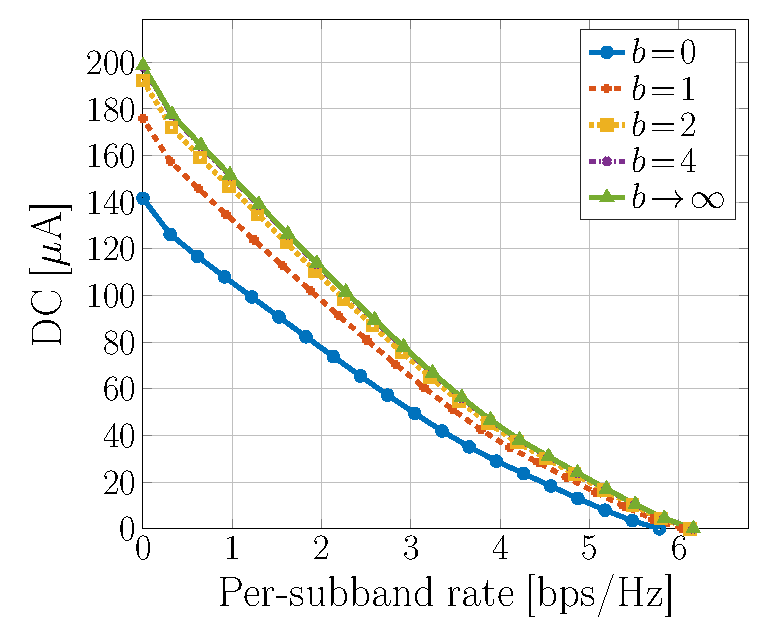
\includegraphics{assets/re_quantization.eps}
				% This file was created by matlab2tikz.
%
%The latest updates can be retrieved from
%  http://www.mathworks.com/matlabcentral/fileexchange/22022-matlab2tikz-matlab2tikz
%where you can also make suggestions and rate matlab2tikz.
%
\definecolor{mycolor1}{rgb}{0.00000,0.44700,0.74100}%
\definecolor{mycolor2}{rgb}{0.85000,0.32500,0.09800}%
\definecolor{mycolor3}{rgb}{0.92900,0.69400,0.12500}%
\definecolor{mycolor4}{rgb}{0.49400,0.18400,0.55600}%
\definecolor{mycolor5}{rgb}{0.46600,0.67400,0.18800}%
%
\begin{tikzpicture}

\begin{axis}[%
width=4.036in,
height=3.396in,
at={(0.677in,0.458in)},
scale only axis,
xmin=0,
xlabel style={font=\color{white!15!black}},
xlabel={Per-subband rate [bps/Hz]},
ymin=0,
ylabel style={font=\color{white!15!black}},
ylabel={DC [$\mu$A]},
axis background/.style={fill=white},
xmajorgrids,
ymajorgrids,
legend style={legend cell align=left, align=left, draw=white!15!black},
title style={font=\huge}, label style={font=\huge}, ticklabel style={font=\LARGE}, legend style={font=\LARGE}
]
\addplot [color=mycolor1, line width=2.0pt, mark=o, mark options={solid, mycolor1}]
  table[row sep=crcr]{%
5.78128456302125	0\\
5.47700733355951	3.47479822633982\\
5.17273025639883	7.97550683456363\\
4.86845468081382	13.0200654140677\\
4.56417834752466	18.3360817148957\\
4.25989907004786	23.7318384562944\\
3.95562111705288	29.0279402229329\\
3.6513446531485	35.1277176855932\\
3.347069902469	41.9513454112586\\
3.04279547054435	49.4780718118315\\
2.73852382995822	57.3227833752163\\
2.43425583240962	65.5143296465977\\
2.1299948971445	73.8735219878066\\
1.82573416031542	82.3108459744559\\
1.52147264406495	90.8423097379968\\
1.21720288662051	99.3939878531132\\
0.912934495165668	107.992933349717\\
0.608658453520355	116.829886834298\\
0.30437058100917	126.269131502503\\
0.000154677204868948	141.651203532614\\
};
\addlegendentry{$b = 0$}

\addplot [color=mycolor2, dashed, line width=2.0pt, mark=+, mark options={solid, mycolor2}]
  table[row sep=crcr]{%
6.03179092530422	2.84218744779706e-15\\
5.70895317748491	4.15518954147179\\
5.3866524635236	9.60592132441092\\
5.06504162244455	15.6783914719032\\
4.74408265399704	22.0291232027791\\
4.4239568153569	28.3988551793528\\
4.10394311789509	34.8255063048628\\
3.78414375909185	42.4729111248762\\
3.4648418251932	51.169231591952\\
3.14572562967583	60.5835289574384\\
2.826633049696	70.5776641168941\\
2.50852597847188	80.9017980360601\\
2.19114183643849	91.370052483165\\
1.87470504493036	102.041081593347\\
1.55891720652745	112.94154673888\\
1.24406471268125	123.833871391127\\
0.930192743624454	134.875212156386\\
0.617743372234294	145.884301941296\\
0.307045292317033	157.489053199023\\
4.25721510420636e-06	175.860533456636\\
};
\addlegendentry{$b = 1$}

\addplot [color=mycolor3, dotted, line width=2.0pt, mark=square, mark options={solid, mycolor3}]
  table[row sep=crcr]{%
6.12553634086861	2.97891644196612e-15\\
5.8016683974005	4.39162669859055\\
5.47792410186743	10.1852845728344\\
5.15434412768303	16.6551061016103\\
4.83092034626884	23.4390273538155\\
4.50782803676152	30.2182741201943\\
4.18476638650007	37.1321859955918\\
3.86163094028977	45.4252329370013\\
3.53859475026327	54.8106702738264\\
3.21567544935561	65.0180455154728\\
2.89282013681013	75.8214075688597\\
2.57029633651511	87.0509418846012\\
2.24794215502994	98.6102875172997\\
1.92601520489305	110.547017584343\\
1.60429537519596	122.636231000459\\
1.2828233628442	134.918940463341\\
0.961488097446628	147.015899618792\\
0.640372995288488	159.211502723598\\
0.319592441230883	172.008025229086\\
4.54502906138798e-06	192.201857101392\\
};
\addlegendentry{$b = 2$}

\addplot [color=mycolor4, dashdotted, line width=2.0pt, mark=x, mark options={solid, mycolor4}]
  table[row sep=crcr]{%
6.15924777799679	3.03071377405906e-15\\
5.83496923902249	4.48325587529068\\
5.51071459445702	10.4147321811526\\
5.18649607803011	17.046108002983\\
4.86227732034029	23.9810203741504\\
4.53807463620707	30.9478947296119\\
4.21380356780545	38.0576766858876\\
3.88966045893364	46.5398704758309\\
3.56542578370157	56.1904990089836\\
3.24124085414604	66.6762840589394\\
2.91701001013834	77.7953263599759\\
2.59288098029394	89.372153948655\\
2.26866053888955	101.290884103679\\
1.94450223367231	113.566648611884\\
1.62039543466956	126.104316671878\\
1.2962691075973	138.7009632175\\
0.972113834589741	151.39103480022\\
0.648068727497914	164.064352648109\\
0.324007027828884	177.261082462021\\
4.74530831179947e-06	198.115364913325\\
};
\addlegendentry{$b = 4$}

\addplot [color=mycolor5, line width=2.0pt, mark=triangle, mark options={solid, mycolor5}]
  table[row sep=crcr]{%
6.16150543454348	2.22044604925031e-10\\
5.83721568044417	4.48911840834769\\
5.51292603289668	10.4270574072518\\
5.1886367167884	17.0639725567473\\
4.86434676576325	24.0101520880918\\
4.54005779564508	30.9944766760588\\
4.21576795584817	38.1076518340564\\
3.89147861564078	46.6220103975065\\
3.56718939117116	56.282469215789\\
3.24290039307203	66.7958960003608\\
2.91861147575756	77.9484223296369\\
2.5943237988513	89.5479762047584\\
2.27003549766003	101.484966937522\\
1.94574730432264	113.795171837612\\
1.62145947814017	126.345304070712\\
1.29717210794297	138.995968560333\\
0.972887712370027	151.696996068383\\
0.648606201943072	164.411395054165\\
0.32432139388256	177.647475679368\\
4.75231639373541e-06	198.548182010454\\
};
\addlegendentry{$b \mathrel{\to} \infty$}

\end{axis}
\end{tikzpicture}%

			}
		}
		\caption{Average \gls{r-e} region with imperfect cascaded \gls{csit} and quantized \gls{ris} for $M=1$, $N=16$, $L=20$, $\sigma_n^2=\qty{-40}{dBm}$, $B=\qty{10}{\MHz}$ and $d_{\mathrm{H}}=d_{\mathrm{V}}=\qty{2}{\meter}$. $\epsilon_{n}=0$ and $\epsilon_{n}=\infty$ correspond respectively to perfect \gls{csit} and no \gls{csit} (and random \gls{ris}); $b=0$ and $b \to \infty$ correspond respectively to no \gls{ris} and continuous \gls{ris}.}
	\end{figure}

	We then explore the impacts of imperfect cascaded \gls{csit} and quantized \gls{ris} on the \gls{r-e} performance. Due to the general lack of \gls{rf}-chains at the \gls{ris}, it can be challenging to acquire accurate cascaded \gls{csit} on a short-term basis. We assume the cascaded channel at subband $n$ is
	\begin{equation}
		\boldsymbol{V}_{n} = \hat{\boldsymbol{V}}_{n} + \tilde{\boldsymbol{V}}_{n},
	\end{equation}
	where $\hat{\boldsymbol{V}}_{n}$ is the estimated cascaded \gls{csit} and $\tilde{\boldsymbol{V}}_{n}$ is the estimation error with entries following i.i.d. \gls{cscg} distribution $\mathcal{CN}(0, \epsilon_{n}^2)$.\footnote{Note that the subchannel responses are correlated but the estimations can be independent.} Figure~\subref*{fi:re_csi} shows that the proposed passive beamforming Algorithm~\ref{al:sca} is robust to cascaded \gls{csit} inaccuracy for broadband \gls{swipt} with different $L$. On the other hand, since the practical reflection coefficient depends on the available element impedances, we consider a discrete \gls{ris} codebook $\mathcal{C}_\phi = \{e^{j 2 \pi i / 2^b} \mid i = 1, \dots, 2^b\}$ and uniformly quantize the continuous reflection coefficients obtained by Algorithm~\ref{al:bcd} to reduce the circuit complexity and control overhead.\footnote{This relax-then-quantize approach can bring notable performance loss compared with direct optimization over the discrete phase shift set, especially for a small $b$ (i.e., low-resolution \gls{ris}) \cite{Wu2020c}.} Figure~\subref*{fi:re_quantization} suggests that even $b=1$ (i.e., two-state reflection) brings considerable \gls{r-e} gain over the benchmark scheme without \gls{ris}, and the performance gap between $b=4$ and unquantized \gls{ris} is negligible. These observations demonstrate the advantage of the proposed joint waveform, active and passive beamforming design in practical \gls{ris}-aided \gls{swipt} systems.
\end{section}


\begin{section}{Conclusion and Future Works}\label{se:conclusion_and_future_works}
	This paper investigated the \gls{r-e} tradeoff of a single user employing practical receiving strategies in a \gls{ris}-aided multi-carrier \gls{miso} \gls{swipt} system. Uniquely, we considered the joint waveform, active and passive beamforming design under rectifier nonlinearity to maximize the achievable \gls{r-e} region. A three-stage \gls{bcd} algorithm was proposed to solve the problem. In the first stage, the \gls{ris} phase shift was obtained by the \gls{sca} technique and eigen decomposition. In the second and third stages, the active precoder was derived in closed form, and the waveform amplitude and splitting ratio were optimized by the \gls{gp} method. We also proposed and combined closed-form adaptive waveform schemes with a modified passive beamforming strategy to formulate a low-complexity \gls{bcd} algorithm that achieves a good balance between performance and complexity. Numerical results revealed significant \gls{r-e} gains by modeling harvester nonlinearity in the \gls{ris}-aided \gls{swipt} design. Unlike active antennas, \gls{ris} elements cannot be designed independently across frequencies, but can integrate coherent combining and equal gain transmission to enable constructive reflection and flexible subchannel design. Compared to the conventional no-\gls{ris} system, the \gls{ris} mainly affects the effective channel instead of the waveform design.

	One particular unanswered question of this paper is how to design waveform, active and passive beamforming in a multi-user multi-carrier \gls{ris}-aided \gls{swipt} system. Also, harvester saturation effect and practical \gls{ris} models with amplitude-phase coupling \cite{Abeywickrama2020}, angle-dependent reflection \cite{Tang2021}, frequency-dependent reflection, and/or partially/fully-connected architecture \cite{Shen2020a} could be considered in future works.
\end{section}
